\documentclass[12pt,twoside]{report}

%%%%%%%%%%%%%%%%%%%%%%%%%%%%%%%%%%%%%%%%%%%%%%%%%%%%%%%%%%%%%%%%%%%%%%%%%%%%%

% Definitions for the title page
% Edit these to provide the correct information
% e.g. \newcommand{\reportauthor}{Timothy Kimber}

\newcommand{\reporttitle}{Identificación del tipo de tumor en mamografías}
\newcommand{\reportauthor}{}
\newcommand{\degreetype}{Doble Grado Ingeniería Informática y Matemáticas}

%%%%%%%%%%%%%%%%%%%%%%%%%%%%%%%%%%%%%%%%%%%%%%%%%%%%%%%%%%%%%%%%%%%%%%%%%%%%%

% load some definitions and default packages
%%%%%%%%%%%%%%%%%%%%%%%%%%%%%%%%%%%%%%%%%
% University Assignment Title Page 
% LaTeX Template
% Version 1.0 (27/12/12)
%
% This template has been downloaded from:
% http://www.LaTeXTemplates.com
%
% Original author:
% WikiBooks (http://en.wikibooks.org/wiki/LaTeX/Title_Creation)
%
% License:
% CC BY-NC-SA 3.0 (http://creativecommons.org/licenses/by-nc-sa/3.0/)
% 
%
%%%%%%%%%%%%%%%%%%%%%%%%%%%%%%%%%%%%%%%%%
%----------------------------------------------------------------------------------------
%	PACKAGES AND OTHER DOCUMENT CONFIGURATIONS
%----------------------------------------------------------------------------------------
\usepackage[a4paper,hmargin=2.8cm,vmargin=2.0cm,includeheadfoot]{geometry}
\usepackage{textpos}
\usepackage{tabularx,longtable,multirow,subfigure,caption}%hangcaption
\usepackage{fncylab} %formatting of labels
\usepackage{fancyhdr} % page layout
\usepackage{url} % URLs
\usepackage[english]{babel}
\usepackage{amsmath}
\usepackage{graphicx}
\usepackage{dsfont}
\usepackage{epstopdf} % automatically replace .eps with .pdf in graphics
\usepackage{array}
\usepackage{latexsym}
\usepackage{booktabs}
\usepackage[pdftex,hypertexnames=false,colorlinks]{hyperref} % provide links in pdf
\usepackage[
    type={CC},
    modifier={by-nc-sa},
    version={3.0},
]{doclicense}
\usepackage[
backend=bibtex,
style=alphabetic,
sorting=ynt
]{biblatex}
\addbibresource{refs.bib}

\usepackage{listings}
\usepackage{color}
\usepackage{multicol}
\definecolor{dkgreen}{rgb}{0,0.6,0}
\definecolor{gray}{rgb}{0.5,0.5,0.5}
\definecolor{mauve}{rgb}{0.58,0,0.82}

\lstset{frame=tb,
  language=Python,
  aboveskip=0.5mm,
  belowskip=0.5mm,
  showstringspaces=false,
  columns=flexible,
  basicstyle={\small\ttfamily},
  numbers=none,
  numberstyle=\tiny\color{gray},
  keywordstyle=\color{blue},
  commentstyle=\color{dkgreen},
  stringstyle=\color{mauve},
  breaklines=true,
  breakatwhitespace=true,
  tabsize=1
}

\hypersetup{pdftitle={},
  pdfsubject={}, 
  pdfauthor={},
  pdfkeywords={}, 
  pdfstartview=FitH,
  pdfpagemode={UseOutlines},% None, FullScreen, UseOutlines
  bookmarksnumbered=true, bookmarksopen=true, colorlinks,
    citecolor=black,%
    filecolor=black,%
    linkcolor=black,%
    urlcolor=black}

\usepackage[all]{hypcap}


%\usepackage{color}
%\usepackage[tight,ugly]{units}
%\usepackage{float}
%\usepackage{tcolorbox}
%\usepackage[colorinlistoftodos]{todonotes}
% \usepackage{ntheorem}
% \theoremstyle{break}
% \newtheorem{lemma}{Lemma}
% \newtheorem{theorem}{Theorem}
% \newtheorem{remark}{Remark}
% \newtheorem{definition}{Definition}
% \newtheorem{proof}{Proof}


%%% Default fonts
\renewcommand*{\rmdefault}{bch}
\renewcommand*{\ttdefault}{cmtt}
\renewcommand{\contentsname}{Índice}

%%% Default settings (page layout)
\setlength{\parindent}{0em}  % indentation of paragraph

\setlength{\headheight}{14.5pt}
\pagestyle{fancy}
\renewcommand{\chaptermark}[1]{\markboth{\chaptername\ \thechapter.\ #1}{}} 

\fancyfoot[ER,OL]{\sffamily\textbf{\thepage}}%Page no. in the left on odd pages and on right on even pages
\fancyfoot[OC,EC]{\sffamily }
\renewcommand{\headrulewidth}{0.1pt}
\renewcommand{\footrulewidth}{0.1pt}
\captionsetup{margin=10pt,font=small,labelfont=bf}


%--- chapter heading

\def\@makechapterhead#1{%
  \vspace*{10\p@}%
  {\parindent \z@ \raggedright \sffamily
    \interlinepenalty\@M
    \Huge\bfseries \thechapter \space\space #1\par\nobreak
    \vskip 30\p@
  }}

%---chapter heading for \chapter*  
\def\@makeschapterhead#1{%
  \vspace*{10\p@}%
  {\parindent \z@ \raggedright
    \sffamily
    \interlinepenalty\@M
    \Huge \bfseries  #1\par\nobreak
    \vskip 30\p@
  }}

\allowdisplaybreaks

% load some macros
% Here, you can define your own macros. Some examples are given below.

\newcommand{\R}[0]{\mathds{R}} % real numbers
\newcommand{\Z}[0]{\mathds{Z}} % integers
\newcommand{\N}[0]{\mathds{N}} % natural numbers
\newcommand{\C}[0]{\mathds{C}} % complex numbers
\renewcommand{\vec}[1]{{\boldsymbol{{#1}}}} % vector
\newcommand{\mat}[1]{{\boldsymbol{{#1}}}} % matrix


\date{Curso 2020-2021}

\begin{document}

% load title page
% Last modification: 2015-08-17 (Marc Deisenroth)
\begin{titlepage}

\newcommand{\HRule}{\rule{\linewidth}{0.5mm}} % Defines a new command for the horizontal lines, change thickness here


%----------------------------------------------------------------------------------------
%	LOGO SECTION
%----------------------------------------------------------------------------------------


\includegraphics[width = 4cm]{./figures/ugr}\\[0.5cm] 

\center % Center remainder of the page

%----------------------------------------------------------------------------------------
%	HEADING SECTIONS
%----------------------------------------------------------------------------------------

\textsc{\Large Universidad de Granada}\\[0.5cm] 
\textsc{\large Práctica 1 Inteligencia de Negocio}\\[0.5cm] 

%----------------------------------------------------------------------------------------
%	TITLE SECTION
%----------------------------------------------------------------------------------------

\HRule \\[0.4cm]
{ \huge \bfseries \reporttitle}\\ % Title of your document
\HRule \\[1.5cm]
 
%----------------------------------------------------------------------------------------
%	AUTHOR SECTION
%----------------------------------------------------------------------------------------

\begin{minipage}{0.4\textwidth}
\begin{flushleft} \large
\reportauthor % Your name
\end{flushleft}
\end{minipage}
~


%----------------------------------------------------------------------------------------
%	FOOTER & DATE SECTION
%----------------------------------------------------------------------------------------
\vfill % Fill the rest of the page with whitespace
\degreetype\\[0.5cm]

\makeatletter
\@date 
\makeatother


\end{titlepage}



% page numbering etc.
\pagenumbering{roman}
\clearpage{\pagestyle{empty}\cleardoublepage}
\setcounter{page}{1}
\pagestyle{fancy}


\clearpage{\pagestyle{empty}\cleardoublepage}

%%%%%%%%%%%%%%%%%%%%%%%%%%%%%%%%%%%%
%--- table of contents
\fancyhead[RE,LO]{\sffamily {Table of Contents}}
\begingroup
\pagestyle{plain}
\tableofcontents 
\listoffigures
\listoftables
\endgroup

%\listoftables
\clearpage{\pagestyle{empty}\cleardoublepage}
\pagenumbering{arabic}
\setcounter{page}{1}
\fancyhead[LE,RO]{\slshape \rightmark}
\fancyhead[LO,RE]{\slshape \leftmark}

%%%%%%%%%%%%%%%%%%%%%%%%%%%%%%%%%%%%
\chapter*{Introducción}
\addcontentsline{toc}{chapter}{Introducción}  

El propósito de esta práctica es predecir si  un tumor es benigno o maligno a partir de un conjunto de datos. Se realizarán distintos preprocesamiento sobre los datos, se hara uso de algoritmos de aprendizaje supervisado de clasificación (elegidos con criterio) y un análisis comparado de resultados utilizando distintas medidas de evaluación. Como conjunto de datos se usará el dataset proporcionado por la asignatura que contiene 961 instancias de masas detectadas en mamografías, con 4 atributos numéricos (BI-RADS, Age, Margin y Density) y 2 atributos categóricos (Shape y Severity), donde Severity es nuestro objetivo a predecir.

\begin{enumerate}
	\item Código BI-RADS: sistema de control de calidad, valor numérico 
	\item Age: valor numérico entero
	\item Shape: valor categórico identificado mediante las letras: R redondeada, O Ovalada, L Lobular, I Irregular, N No definida.
	\item Margin: circumscribed=1 microlobulated=2 obscured=3 ill-defined=4 spiculated=5 (nominal)
	\item Density: valor entero ordinal: (1) Alta, (2) Media, (3) Baja, (4) Contenido graso (no tumoral).	
	\item Severity (target, objetivo a predecir): benigno El tumor puede ser de tipo benigno o maligno (cáncer).

\end{enumerate}

Los tipos de algoritmos de clasificación que utilizaremos son \textbf{Regresión Logística} (de los más simples y eficaces para la clasificación de dos clases), \textbf{SVC} (Support Vector Classification, también útiles para clasificación binaria), \textbf{KNeighborsClassifier} y \textbf{Ensemble Clasiffiers} \cite{estimator-choice}. 

El trabajo se realizará sobre el software Scikit-Learn utilizando varios Jupyter Notebook que se adjuntarán en una carpeta llamada \textit{code} junto a este documento.

%%%%%%%%%%%%%%%%%%%%%%%%%%%%%%%%%%%%
\chapter*{Procesado de datos}
\addcontentsline{toc}{chapter}{Procesado de datos}  

En esta sección, haremos una visualización de los datos \footnote{El código para la visualización puede encontrarse en el jupyter notebook data\_visualization.ipynb entregado en la carpeta de code}, probaremos distintos procesados de los misnos, se mostraran resultados y comparaciones con la finalidad de mejorar la predicción teniendo en cuenta validaciones cruzadas de 5 particiones. Principalmente trataremos los valores perdidos y la escala de nuestros datos. En un primer vistazo a nuestro dataset vemos lo siguiente:
\begin{multicols}{2}
\begin{lstlisting}
RangeIndex: 961 entries, 0 to 960
Data columns (total 6 columns):
 #   Column    Non-Null Count  Dtype  
---  ------    --------------  -----  
 0   BI-RADS   959 non-null    float64
 1   Age       956 non-null    float64
 2   Shape     961 non-null    object 
 3   Margin    913 non-null    float64
 4   Density   885 non-null    float64
 5   Severity  961 non-null    object 
dtypes: float64(4), object(2)
\end{lstlisting}
Los algoritmos de Machine Learning no trabajan con strings, por lo que será necesario codificar dichas cadenas como valores numéricos (Shape y Severity).
\columnbreak
\begin{lstlisting}
BI-RADS [ 5.  4.  3. nan  2.  0.  6.]
Age [67. 43. 58. 28. 74. 65. 70. 42. 57. 60. 76. 64. 36. 54. 52. 59. 40. 66.
 56. 75. 63. 45. 55. 46. 39. 81. 77. 48. 78. 50. 61. 62. 44. 23. 80. 53.
 49. 51. 25. 72. 73. 68. 33. 47. 29. 34. 71. 84. 24. 86. 41. 87. 21. 19.
 35. 37. 79. 85. 69. 38. 32. 27. 83. 88. 26. 31. nan 18. 82. 93. 30. 22.
 96. 20.]
Shape ['L' 'R' 'I' 'N' 'O']
Margin [ 5.  1. nan  4.  3.  2.]
Density [ 3. nan  1.  2.  4.]
Severity ['maligno' 'benigno']
\end{lstlisting}
\end{multicols}

En concreto, Severity para que sea un valor numérico binario (maligno 1, benigno 0), también observamos que hay valores perdidos (marcados con nan), concretamente en cada característica tenemos los siguiente valores perdidos, BI-RADS(2), Age(5), Shape(0), Margin(48), Density(76) y Severity(0). Existen un gran número de procedimientos para el tratamiento de valores perdidos, nosotros nos vamos a centrar en \textbf{eliminar} muestras, variables o registros que tienen datos faltantes (hay que tener cuidado y garantizar que los valores descartados no proporcionan información relevante, en nuestro caso veremos que baja el rendimiento de los modelos cuando se incluyen esas instancias ya que solo aportaban ruido al modelo) o \textbf{imputar} valores perdidos mediante distintas técnicas (se pueden sustituir por la media, moda, mediana, etc...).
\\
\\
\\
\\
Visualizamos un poco los datos  \textbf{Fig. [\ref{features-distribucions}]}
\begin{figure}[h]
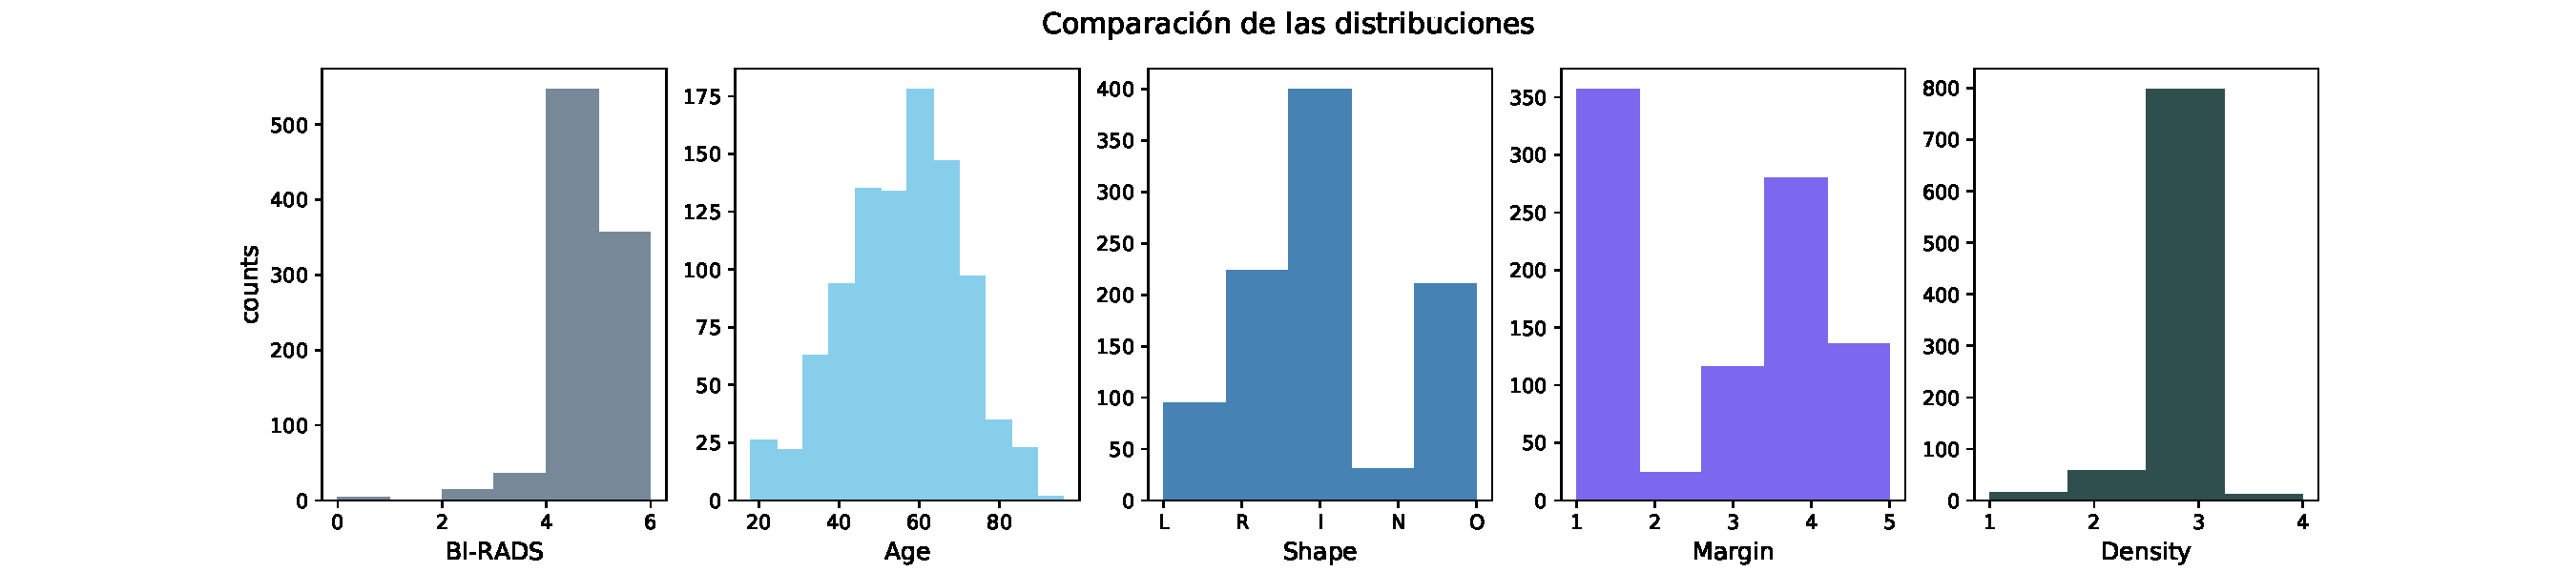
\includegraphics[width=16cm]{./code/figures_python/compare_distribucions.pdf}
\caption{Features distribucions.}
\label{features-distribucions}
\end{figure}

Nuestros datos tienen distintas escalas, la variable Age es la que sigue una distribución mas cercana a la normal, aunque es ligeramente asimétrica a la izquierda. la mayoría ni siquiera siguen la distribución normal, Density y Bi-Raids son muy asimétricas a la izquierda y Shape y Margin tienen dos montañas. Algunos algoritmos de Machine Learning se benefician de la escala de los datos. Por ejemplo, para los modelos que se basan en el cálculo de la distancia (como \textbf{KNeighborsClassifier}), si los datos no estan escalados y una de las características tiene una amplia gama de valores, la distancia se regirá por esta característica en particular y el modelo no funcionará bien. Visualizamos la relación entre Shape y BI-RADS con Severity \textbf{Fig. [\ref{countplots}]}
\begin{figure}[h]
\begin{multicols}{2}
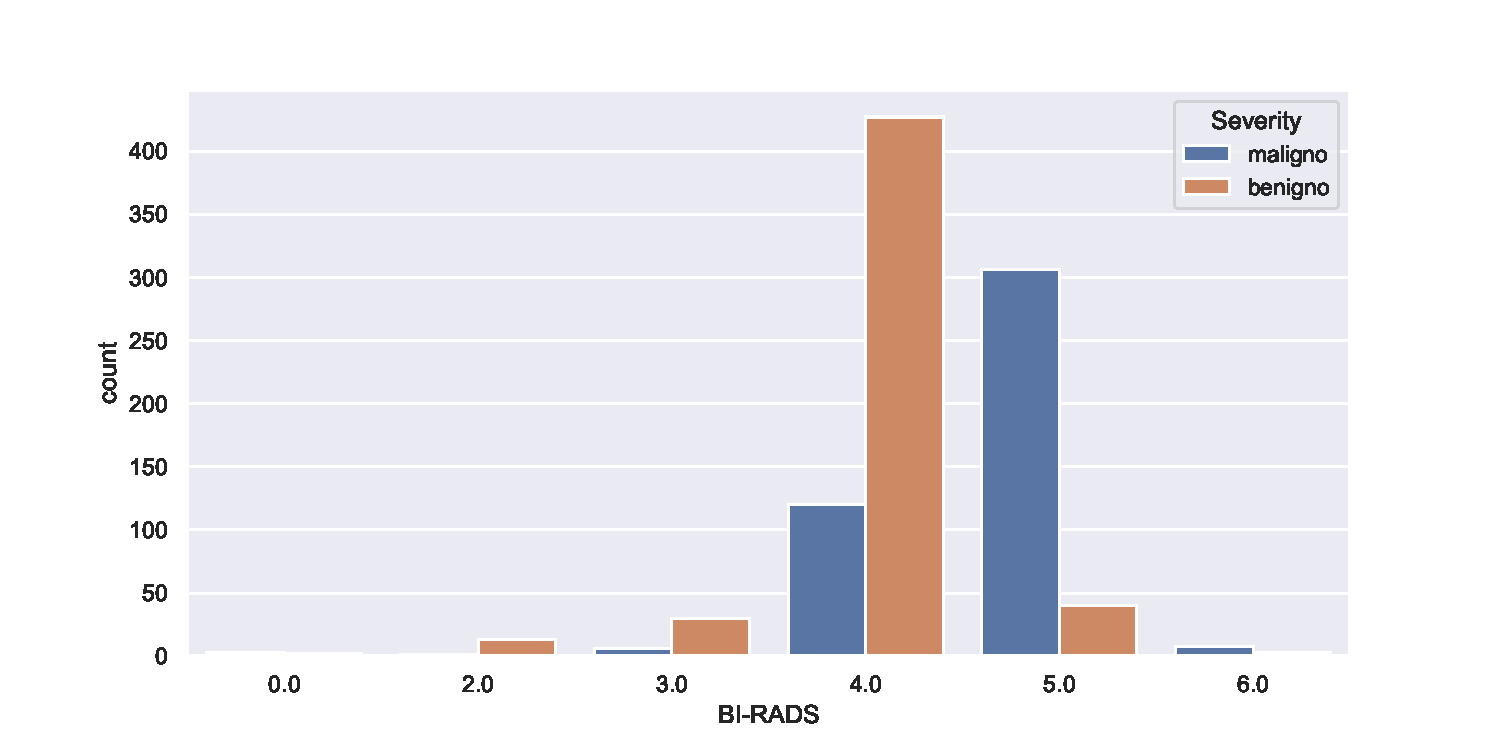
\includegraphics[width=8cm]{./code/figures_python/countplot_bi_severity.pdf}%
\columnbreak
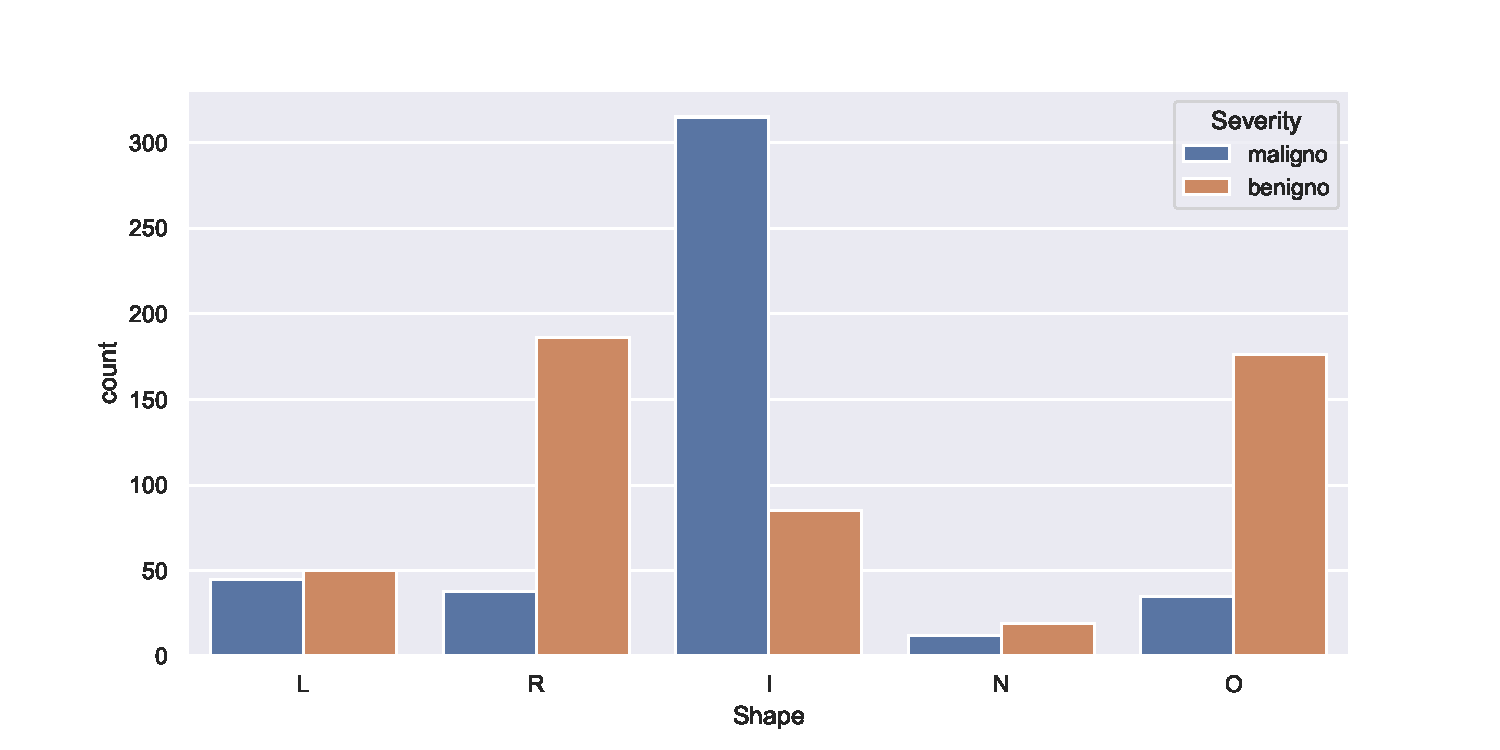
\includegraphics[width=8cm]{./code/figures_python/countplot_shape_severity.pdf}%
\end{multicols}
\caption{Countplots BI-RADS y Shape.}
\label{countplots}
\end{figure}

Veamos la correlación entre nuestras variables, antes codificando Severity y Shape (ya que no son numéricas) con LabelEncoder \cite{label-encoder} (ya que tenemos valores ordinales), veamos la correlación si el orden en el que codificamos Shape es importante o no, (ya que LabelEncoder lo hace en orden alfabético), esencialmente lo único que cambiará será el signo de la correlación, no obtendremos una diferencia muy significativa  que la obtenemos los siguientes mapas de calor \textbf{Fig. [\ref{heatmap}]}, la correlación entre las variables es independiente de que se escalen o no las antes de aplicar la correlación.

\begin{figure}[h]
\begin{multicols}{2}
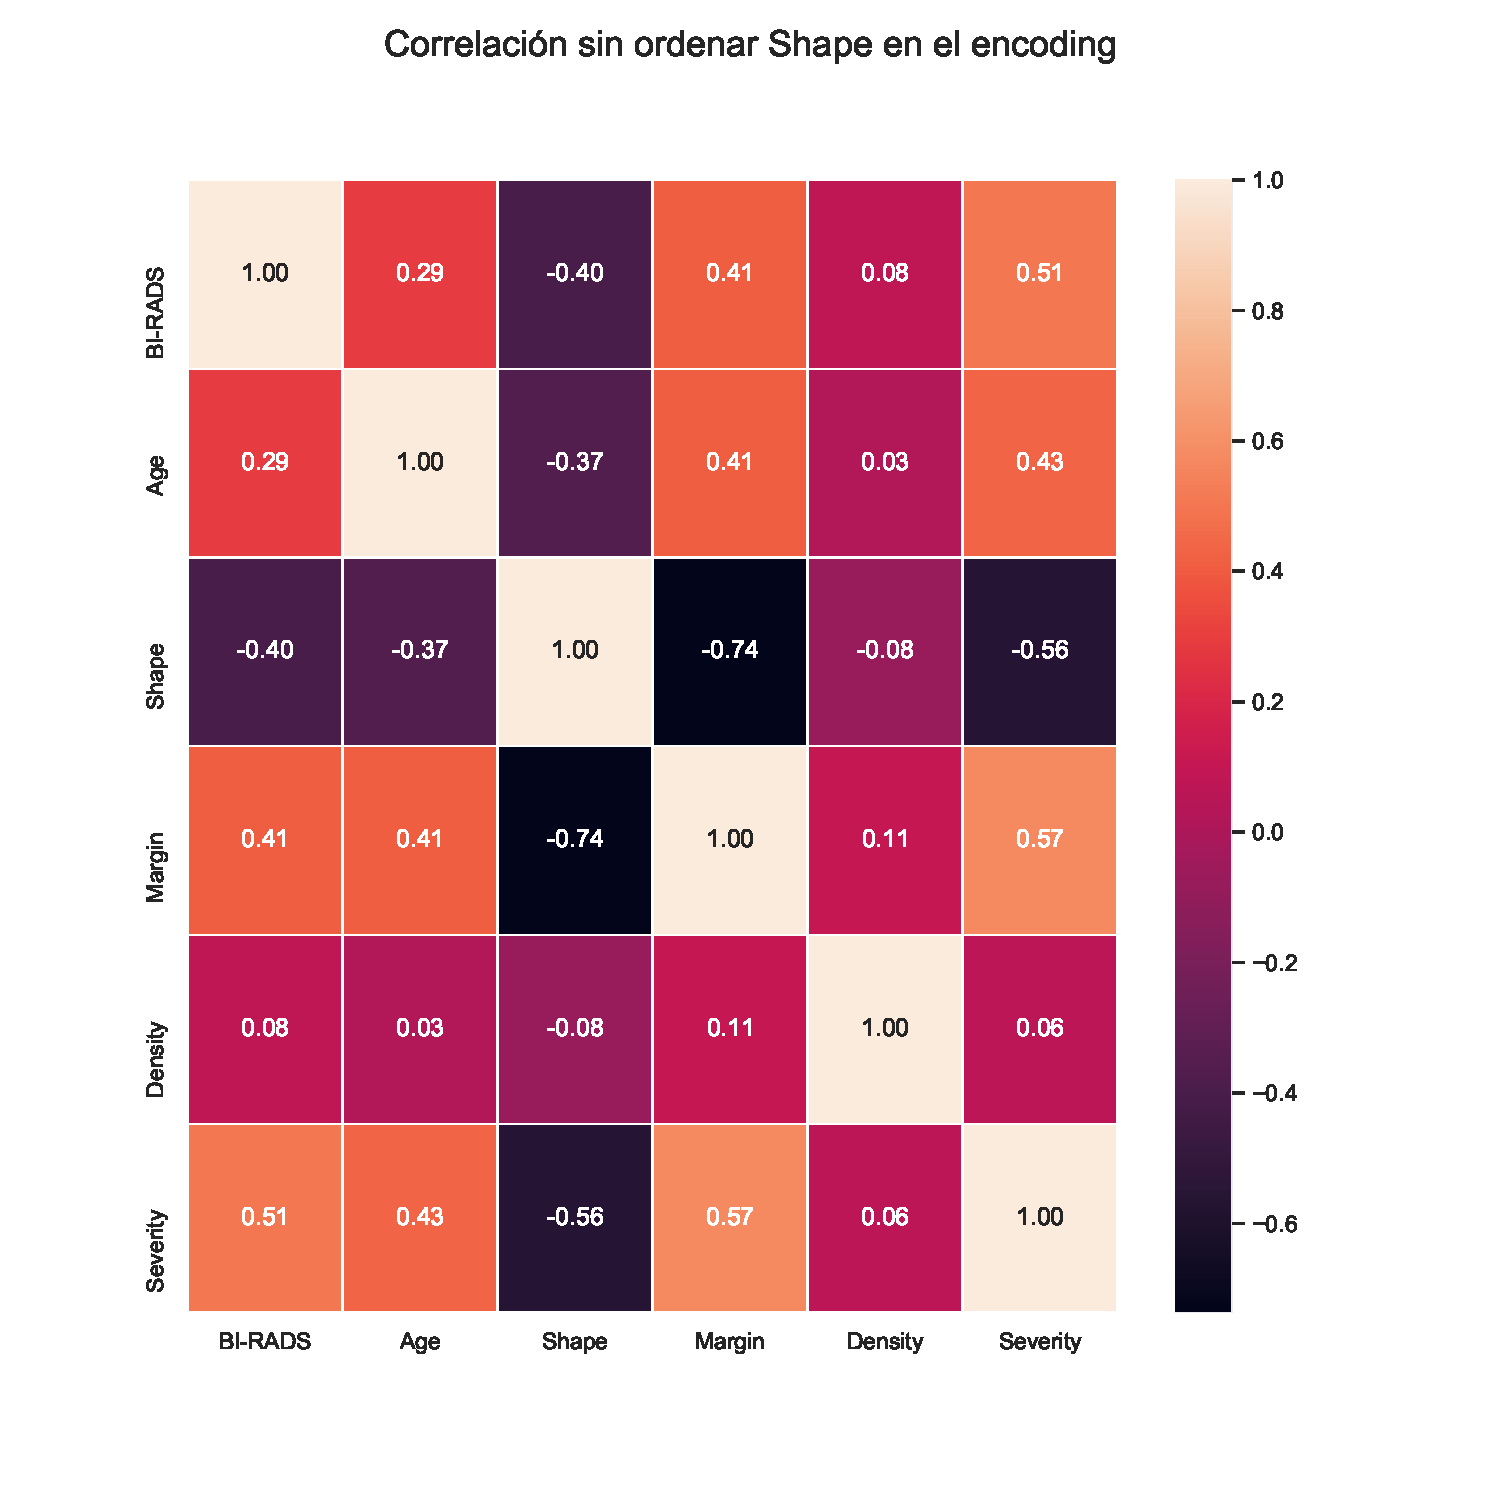
\includegraphics[width=8.5cm]{./code/figures_python/corr.pdf}%
\columnbreak
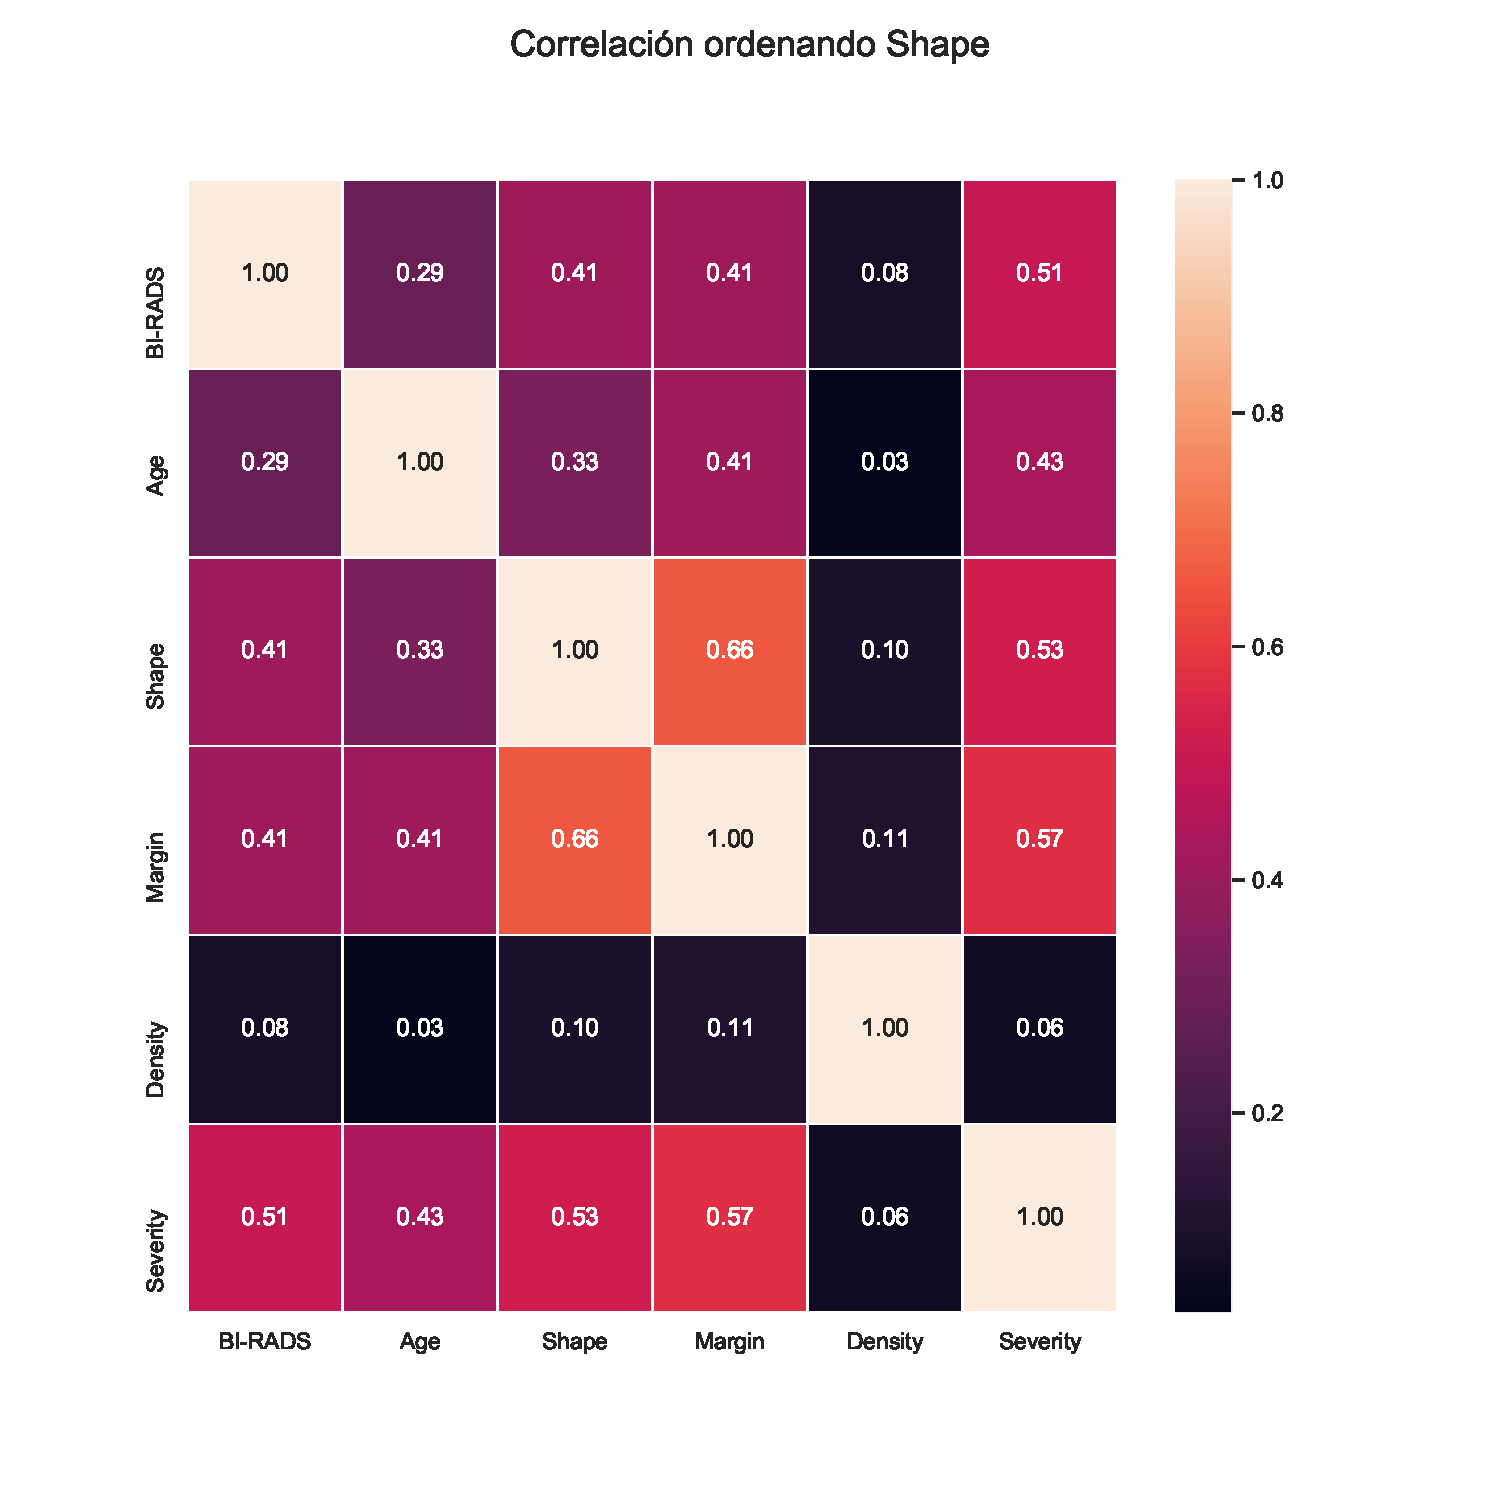
\includegraphics[width=8.5cm]{./code/figures_python/corr_shape_ordered.pdf}%
\end{multicols}
\caption{Heatmap correlation.}
\label{heatmap}
\end{figure}
\vspace{5cm}

\section*{Missing values}
\addcontentsline{toc}{section}{Missing values}  

Estos datos perdidos pueden ser un problema cuando usemos los algoritmos, probaremos distintas tipos de algoritmos de clasificación y configuraciones para los valores perdidos, entre ellas tendremos directamente eliminar todos los valores, \textbf{Drop missing} , la sustitución por la media, \textbf{Mean Imputation}, (solo válido para variables numéricas), mediana, \textbf{Median Imputation} (la mediana es un estimador más robusto para datos con variables de gran magnitud que podrían dominar los resultados, también conocido como \textit{long tail}) y moda, \textbf{Mode Imputation}(solo válido para variables categóricas), del tipo k-vecinos más cercanos, \textbf{KNN Imputation} que consisten en buscar los k valores más próximos al que queremos sustituir. Una vez identificados se puede sustituir por la media (algoritmo k-medias) o por la moda (algoritmo k-modas) e Iterative Imputer, \textbf{Iterative Imputation} (usa regresión lineal round-robin, modelando cada característica con valores perdidos como una función de otras características, la versión implementada asume variables gaussianass, hay que considerar transformarlas para que parezcan más normales y que mejore potencialmente el rendimiento).\footnote{El código para la visualización puede encontrarse en el jupyter notebook imputing\_missing\_values entregado en la carpeta de code},



En la \textbf{Fig. [\ref{imputation}]} mostramos distintas figuras donde comparamos duplas de algoritmos diferentes utilizando como medida accuracy con validación cruzada de 5 particiones. Aunque vemos cada configuración para todos los valores, habría que estudiar cada caracterísitica por separado, por ejemplo, no tiene sentido \textbf{Mean Imputation} para valores no numéricos, utilizaremos pipelines con un preprocesado adecuado para cada caso. No incluimos \textbf{KNeighborsClassifier} ya que habría normalizar los datos en la misma escala (cuando hablamos de normalizar nos referimos a escalar una variable para que tenga valores entre 0 y 1, mientras que la estandarización transforma los datos para que tengan una media de cero y una desviación estándar de 1) al usar distancias, si las variables tienen diferentes escalas, perjudicará al modelo.

\begin{figure}[ht!p]
\caption{Imputation Techniques.}
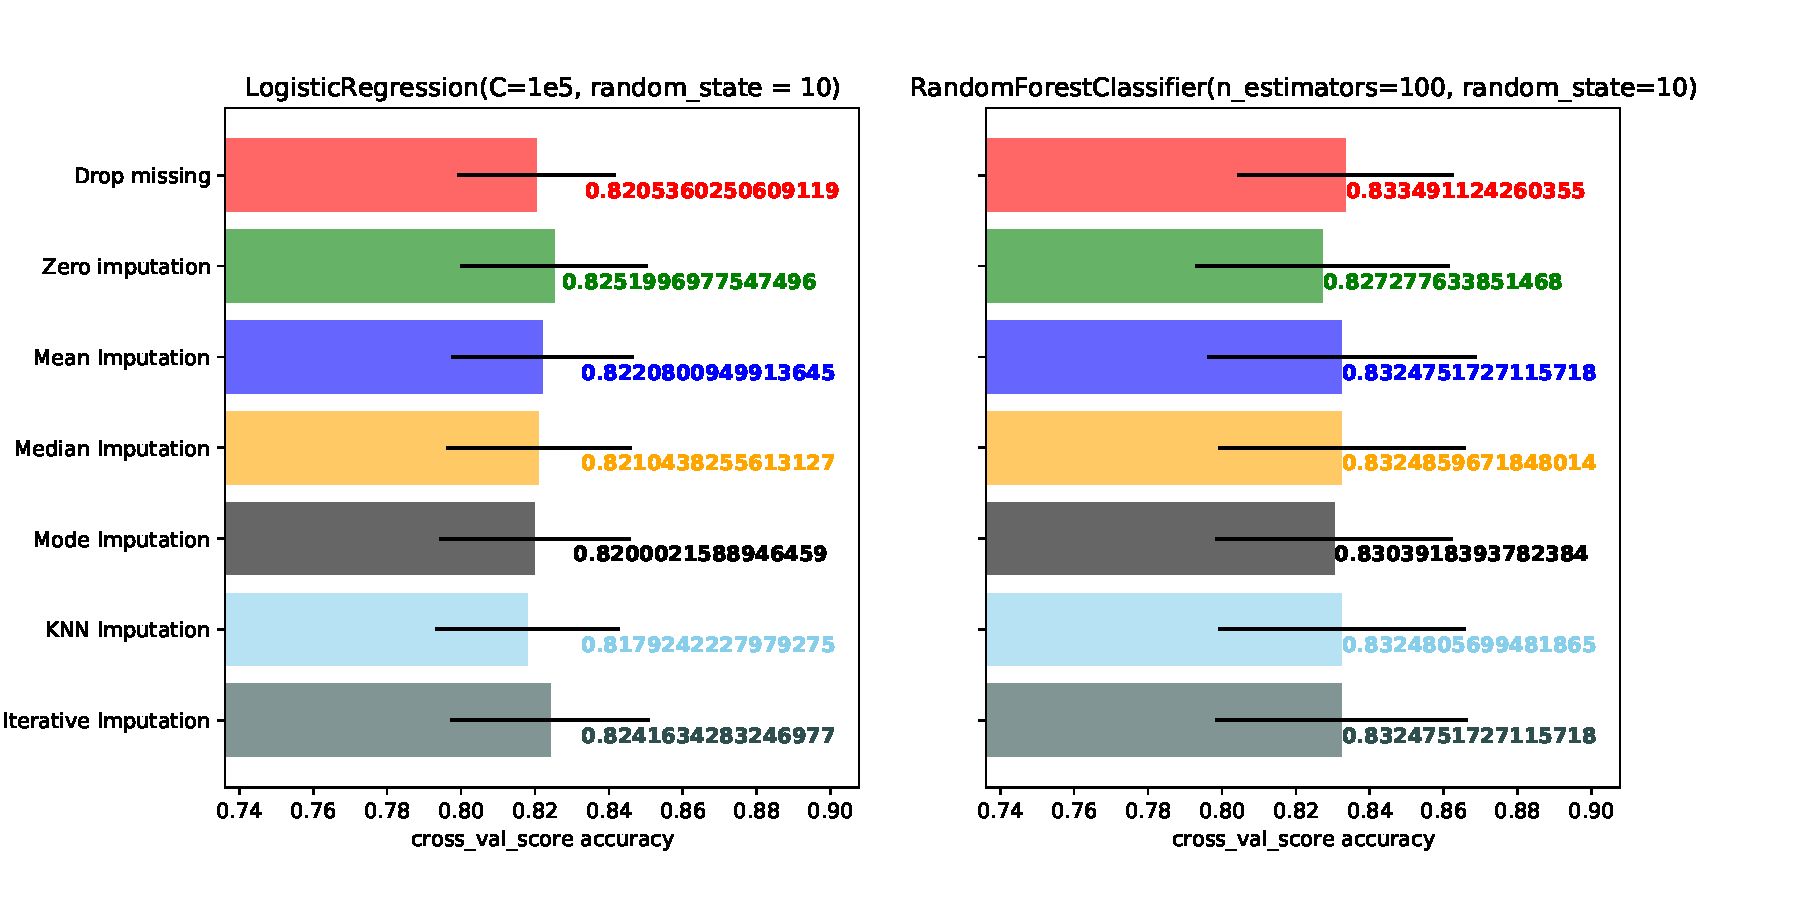
\includegraphics[width=\textwidth]{./code/figures_python/imputation_techniques/imputation_techniques_lr_rfc.pdf}%

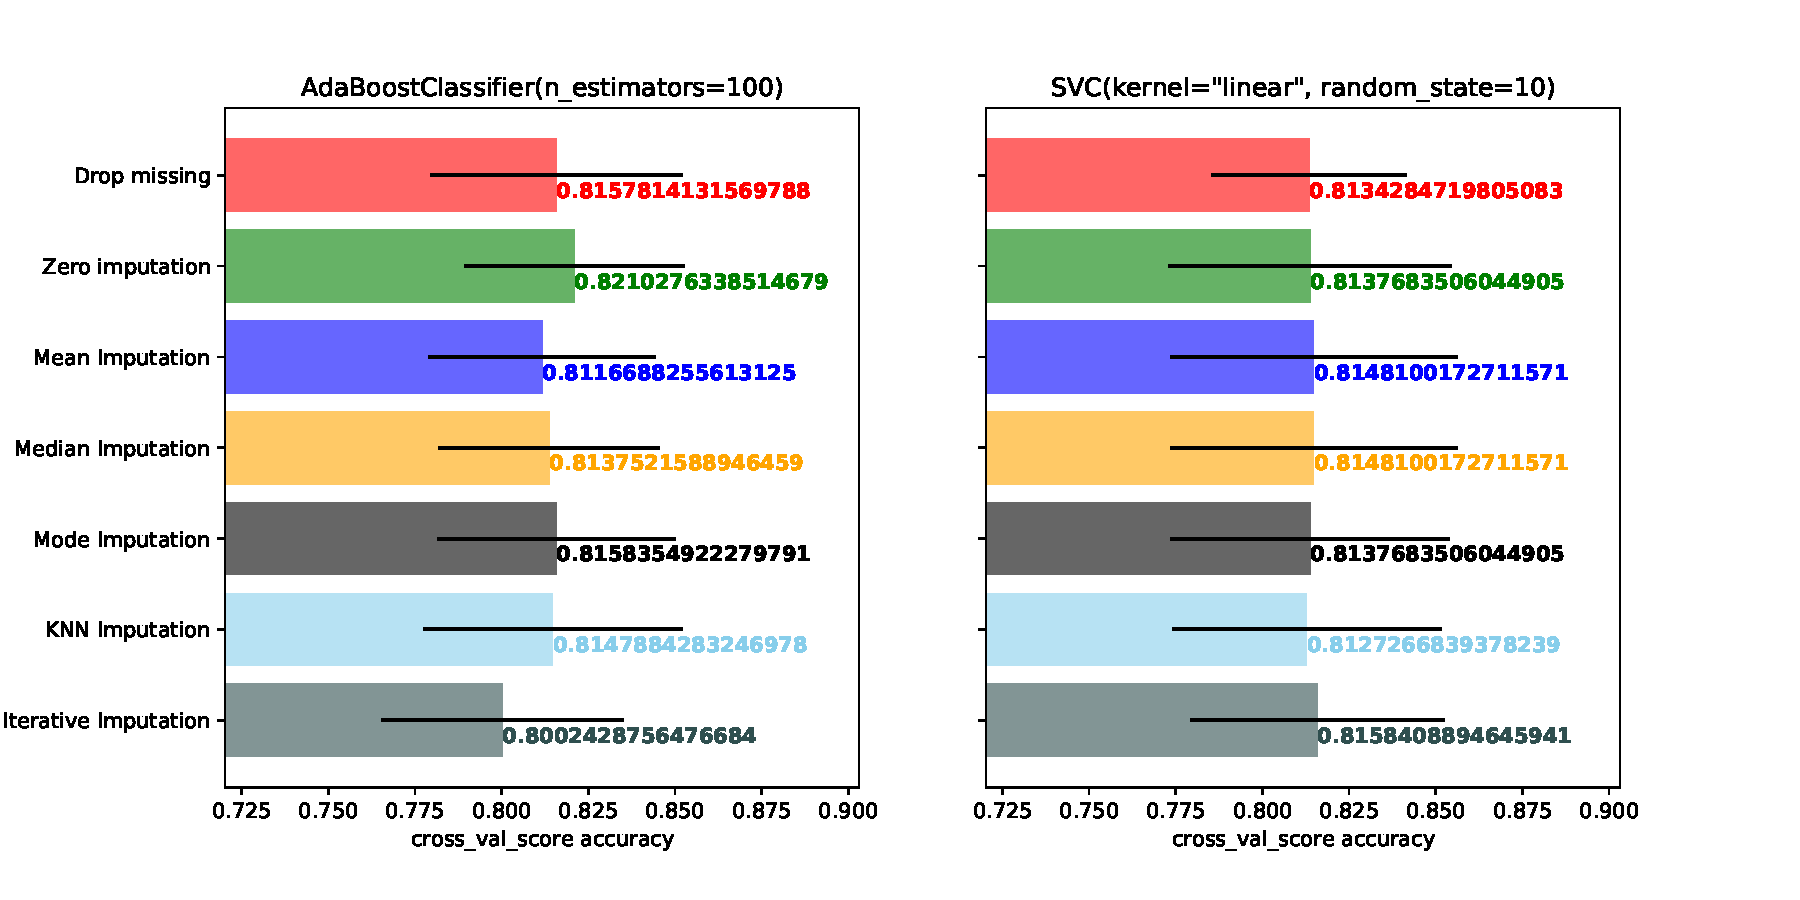
\includegraphics[width=\textwidth]{./code/figures_python/imputation_techniques/imputation_techniques_ab_svc.pdf}%

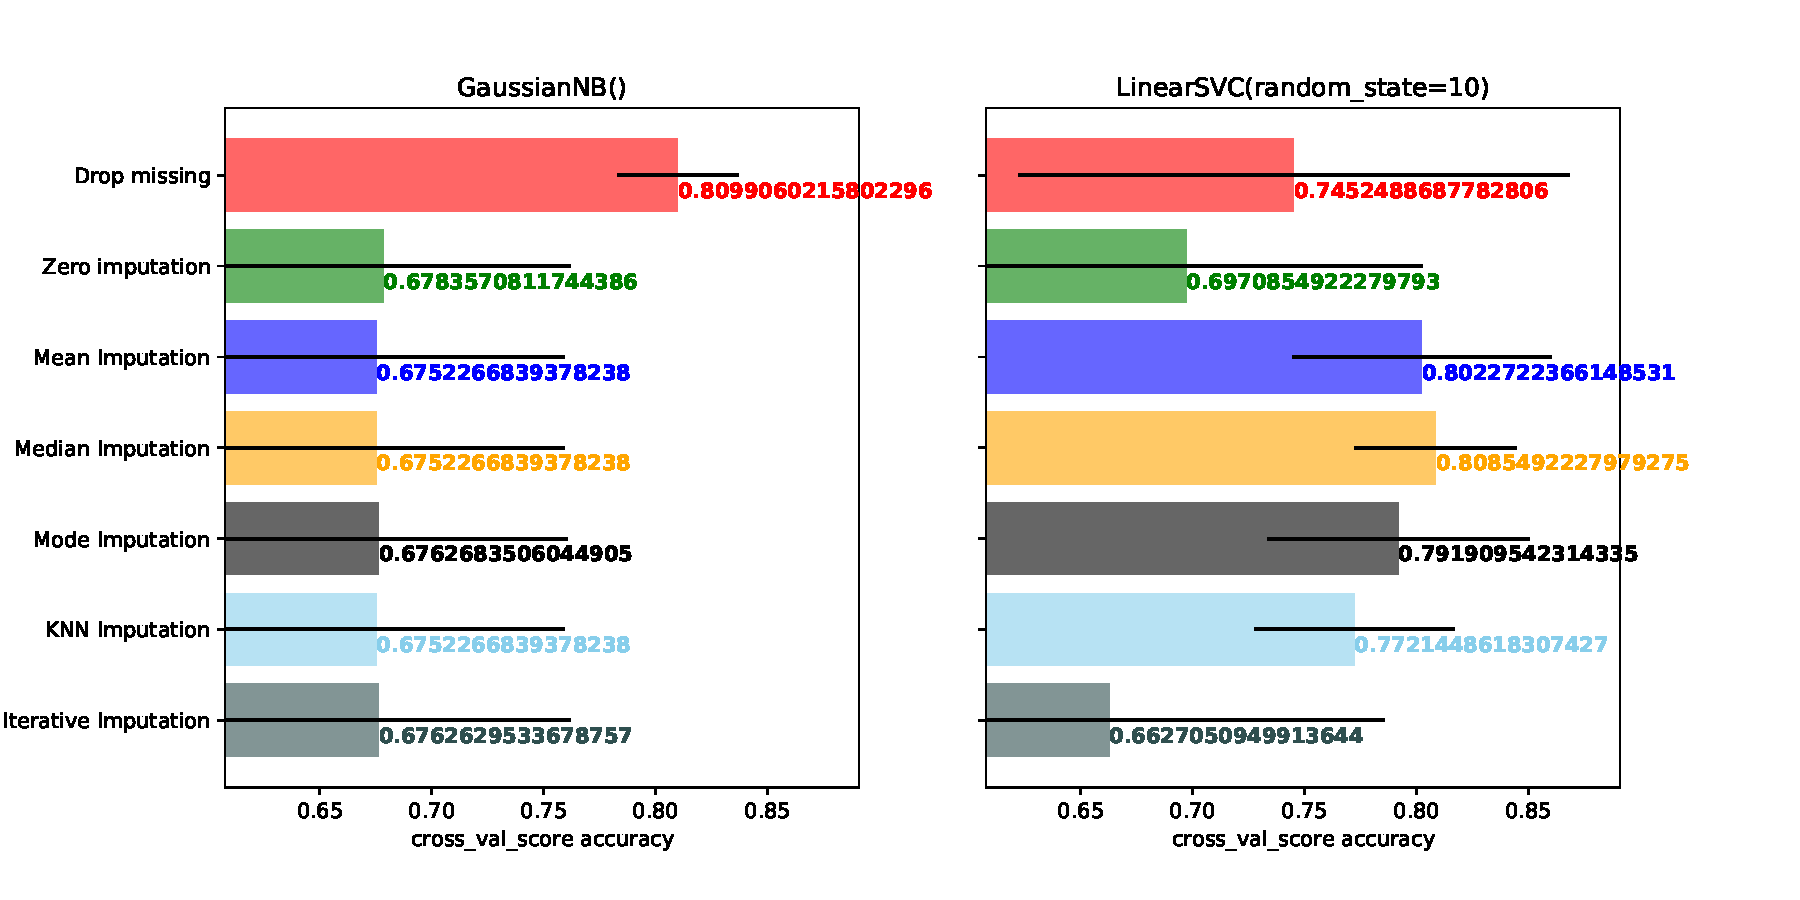
\includegraphics[width=\textwidth]{./code/figures_python/imputation_techniques/imputation_techniques_gnb_svc_linear.pdf}%
\label{imputation}
\end{figure}

\section*{Scaling data}
\addcontentsline{toc}{section}{Scaling data}  

Muchos estimadores tienen el supuesto de que cada característica toma valores cercanos a cero (todas las características varían en escalas comparables). En particular, los estimadores basados en métricas y en gradientes asumen datos estandarizados. Una excepción son los estimadores basados en árboles de decisión que son robustos al escalado arbitrario de datos. Realizaremos lo mismo que antes cambiando los algoritmos elegidos para ver la diferencia entre los datos aplicando estandarización/normalización, incluiremos \textbf{KNeighborsClassifier}, probaremos para distintos tipos de \textbf{SVM} y más modelos \textbf{Naive-Bayes} y eliminaremos los que sabemos que la diferencia es despreciable teniendo en cuenta lo dicho anteriormente.De nuevo adjuntamos una serie de figuras medidas con validación cruzada de 5 particiones donde ponemos los caso que destacamos ya que vemos la variación entre el resultado conseguido dependiendo del tipo de escala de los datos \textbf{Fig. [\ref{imputation-scaled-1}] y [\ref{imputation-scaled-2}]}


Que nuestro estimador Naive-Bayes obtenga malos resultados a pesar del procesado de datos puede ser debido a la dependencia de las variables, aunque no exista correlación entre algunas de nuestras característica sabemos que esto \textbf{no} implica independencia. La elección del número para \textbf{KNeighborsClassifier} se explica en la sección \textbf{[\nameref{section:knn}]}

\begin{figure}[ht!p]
\caption{GaussianNB, MultinomialNB y LinearSVC (Scaled / Normalized)}
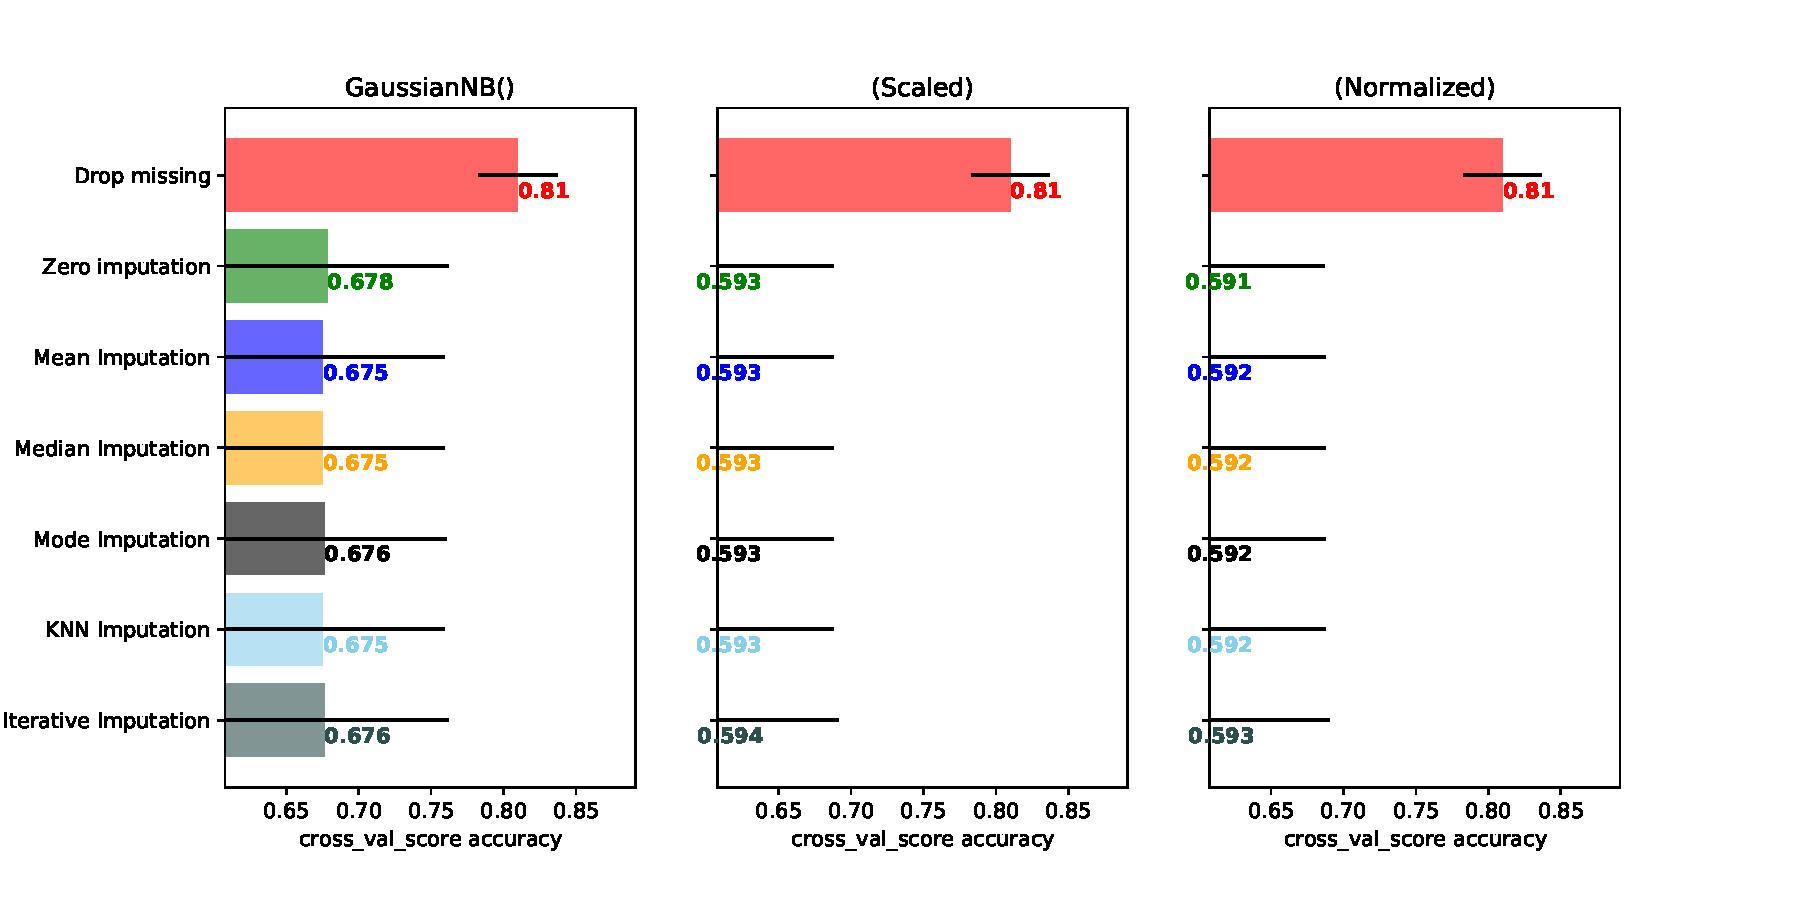
\includegraphics[width=\textwidth]{./code/figures_python/imputation_techniques/imputation_techniques_gnb_scaled_minmax.pdf}%

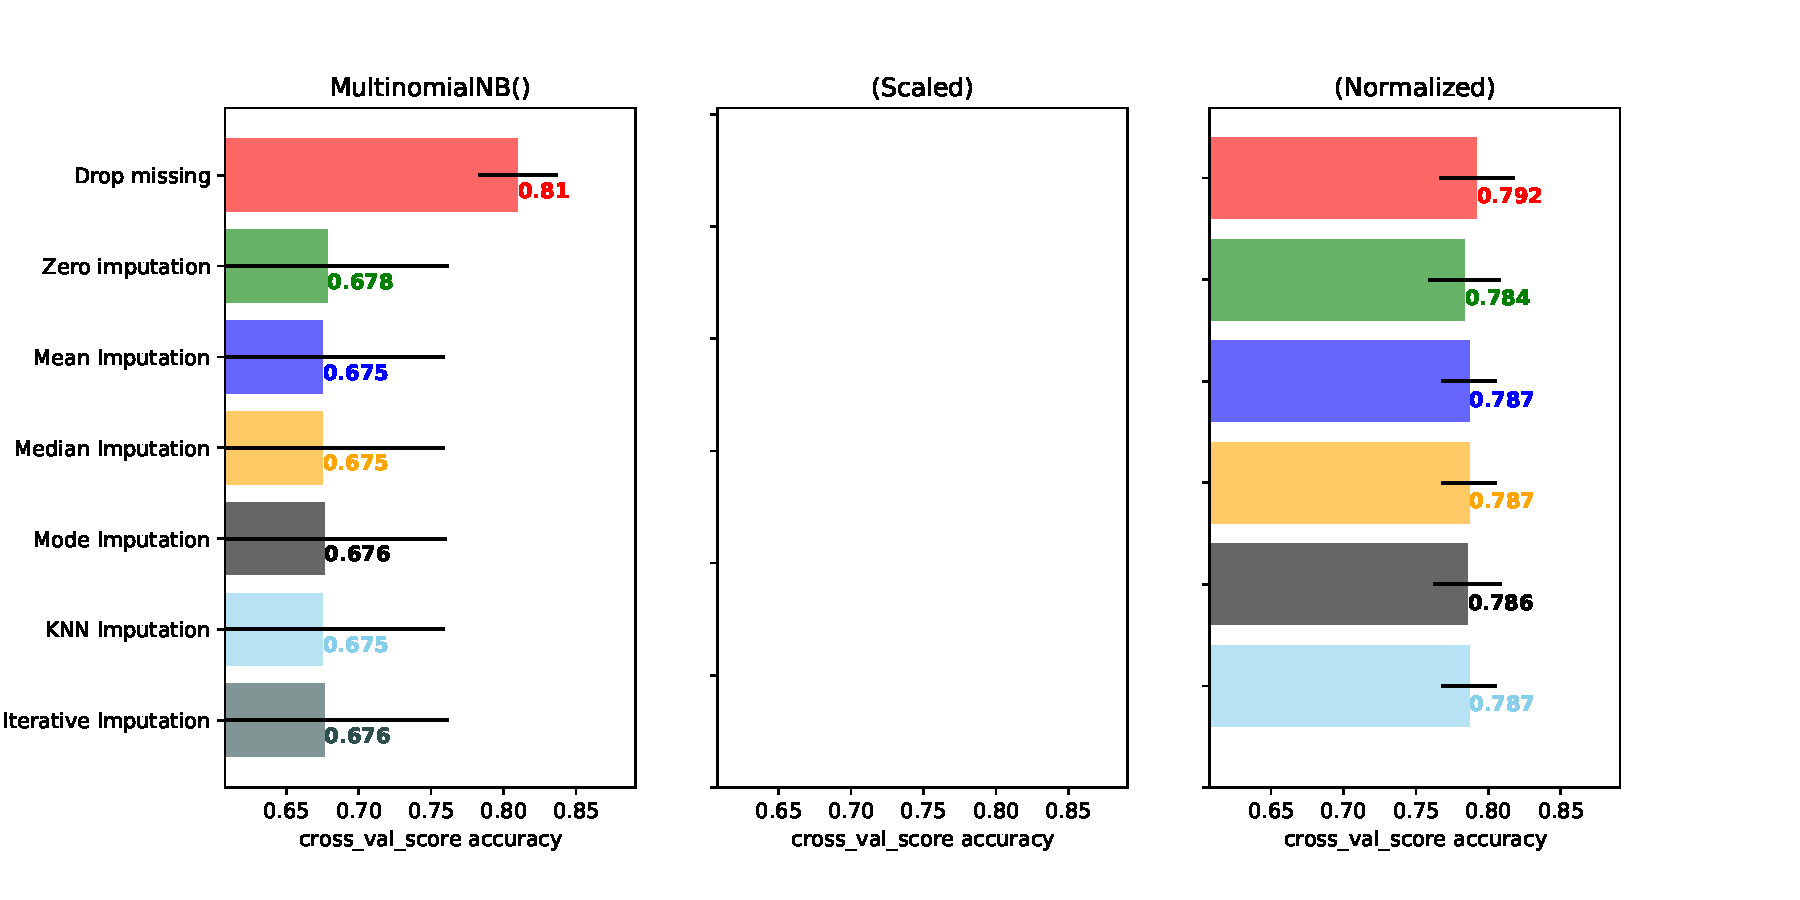
\includegraphics[width=\textwidth]{./code/figures_python/imputation_techniques/imputation_techniques_multinomial_scaled_minmax.pdf}

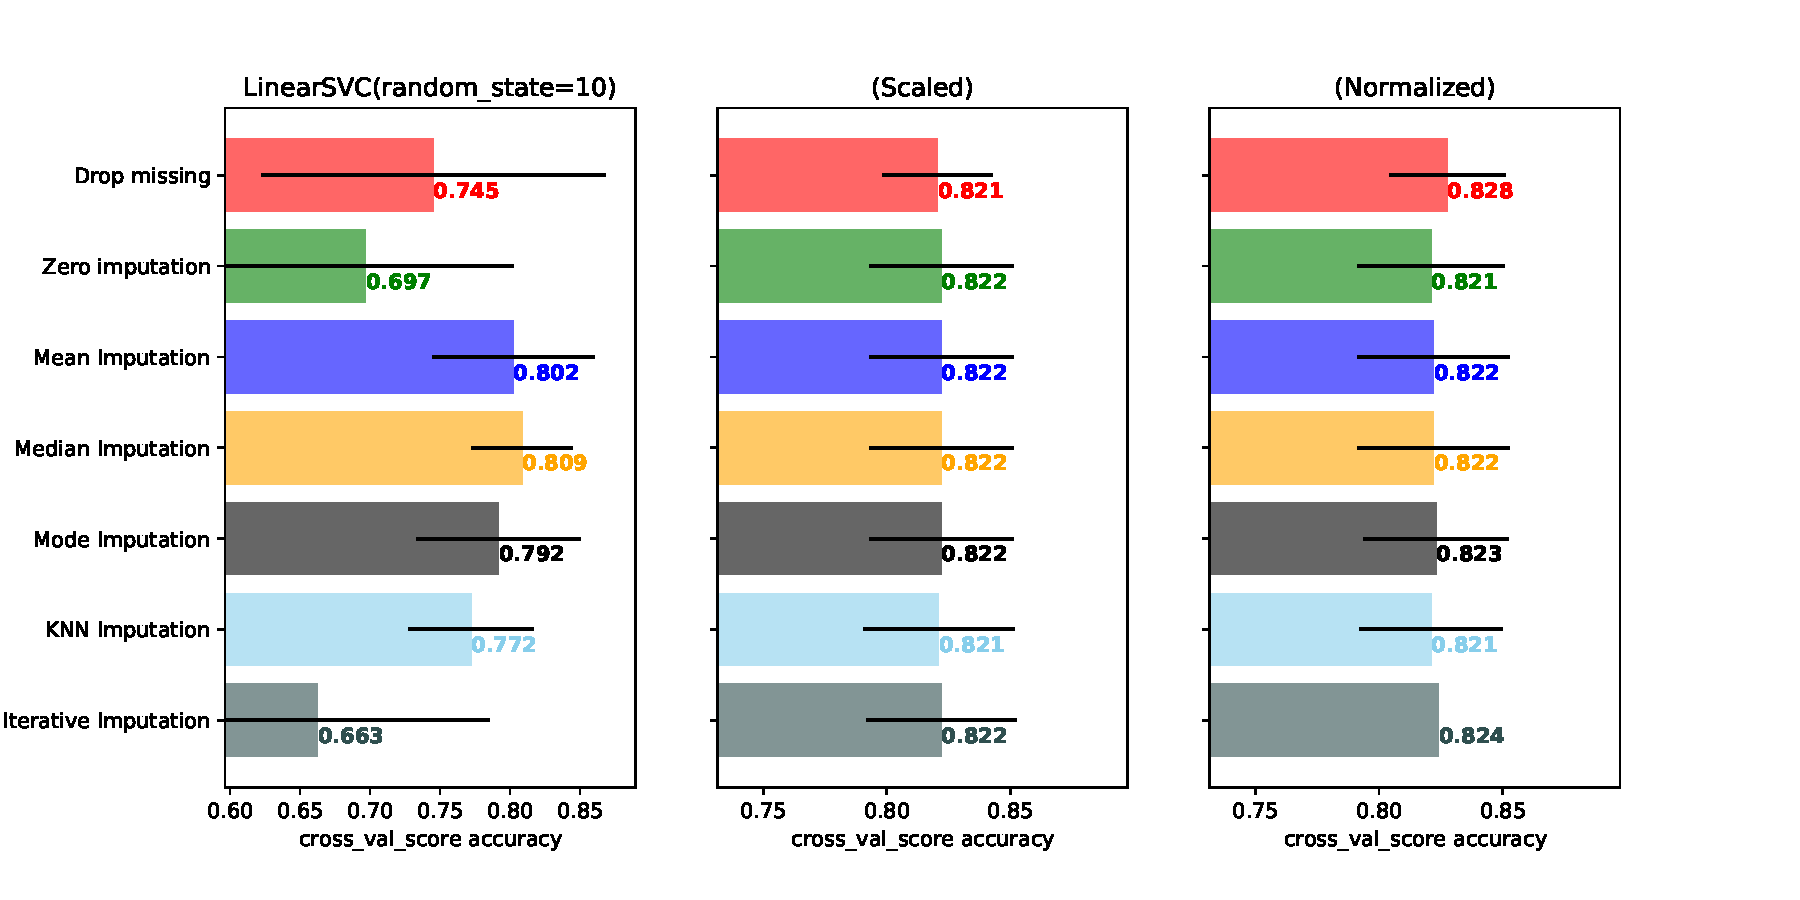
\includegraphics[width=\textwidth]{./code/figures_python/imputation_techniques/imputation_techniques_svc_linear_scaled_minmax.pdf}
\label{imputation-scaled-1}
\end{figure}

\begin{figure}[ht!p]
\caption{GaussianProcessClassifier, KNeighborsClassifier y SVC (Scaled / Normalized)}
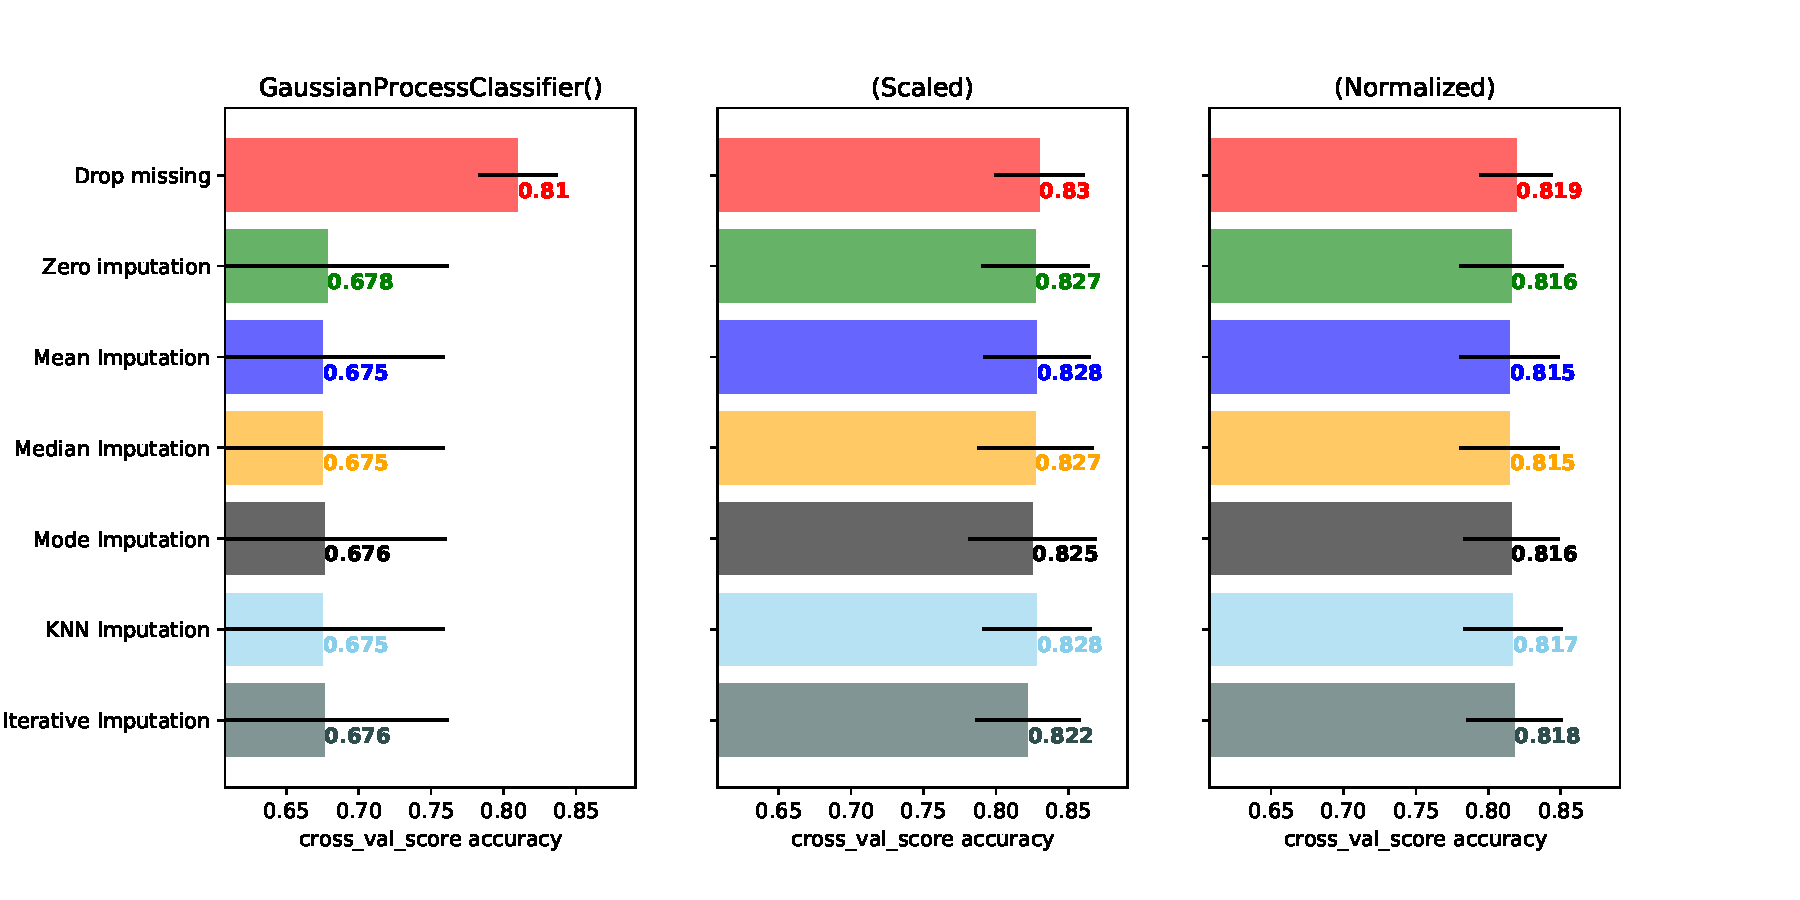
\includegraphics[width=\textwidth]{./code/figures_python/imputation_techniques/imputation_techniques_gpc_scaled_minmax.pdf}%

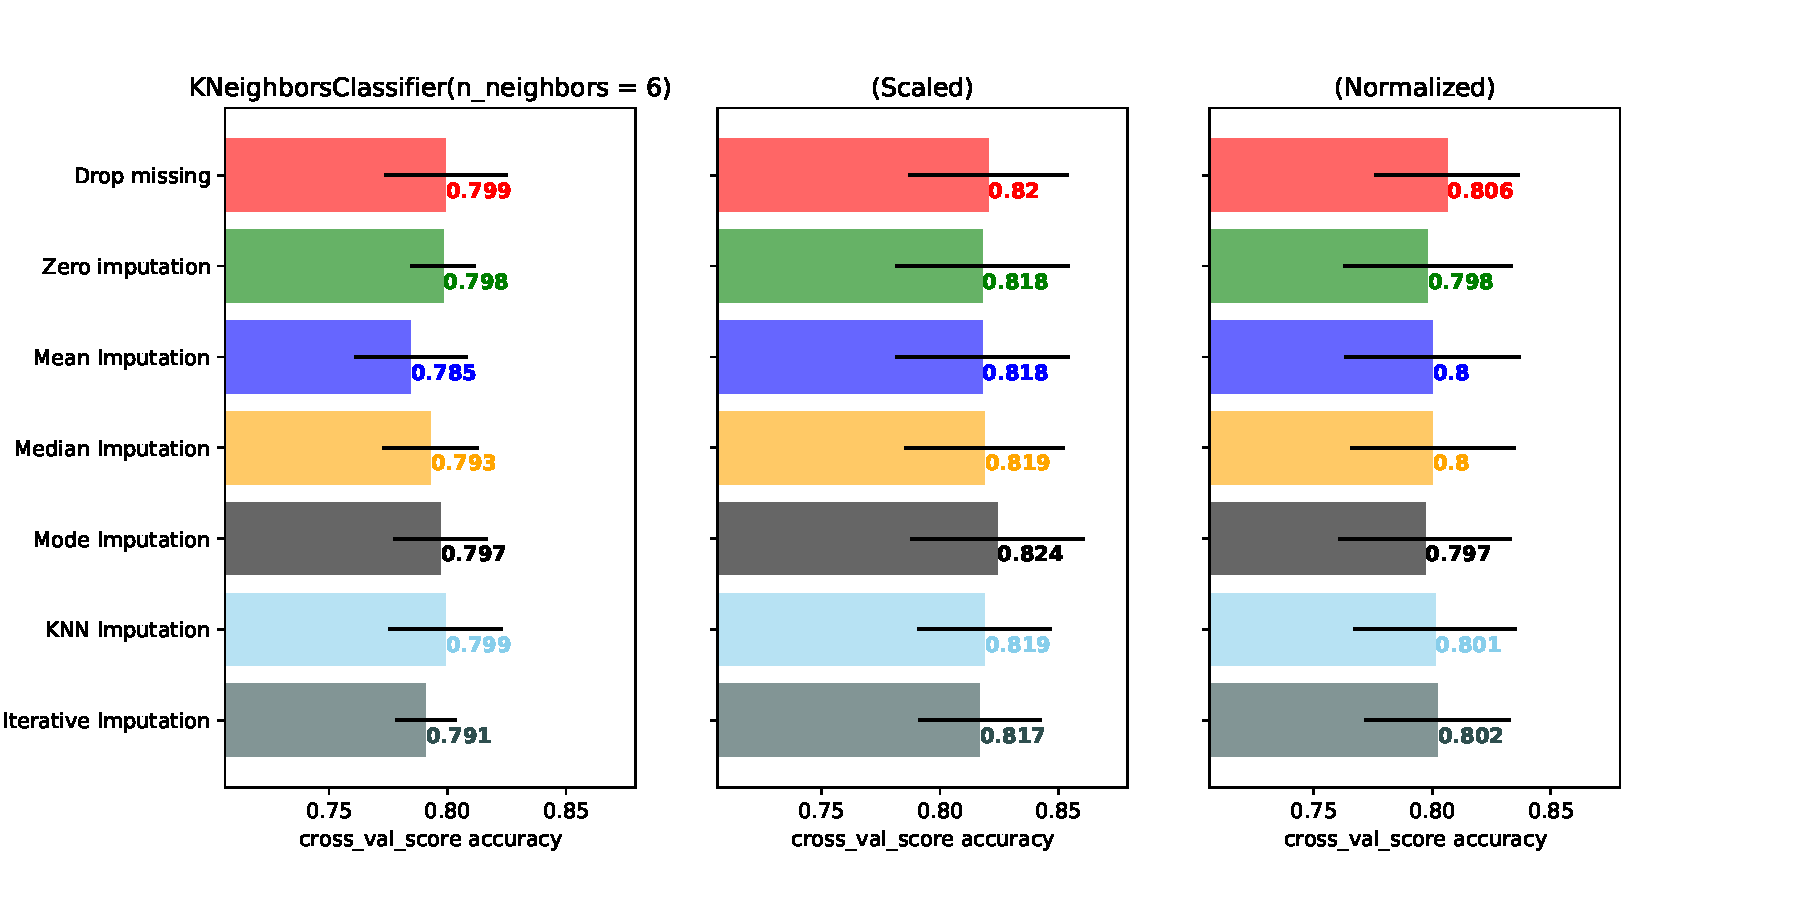
\includegraphics[width=\textwidth]{./code/figures_python/imputation_techniques/imputation_techniques_knn_scaled_minmax.pdf}

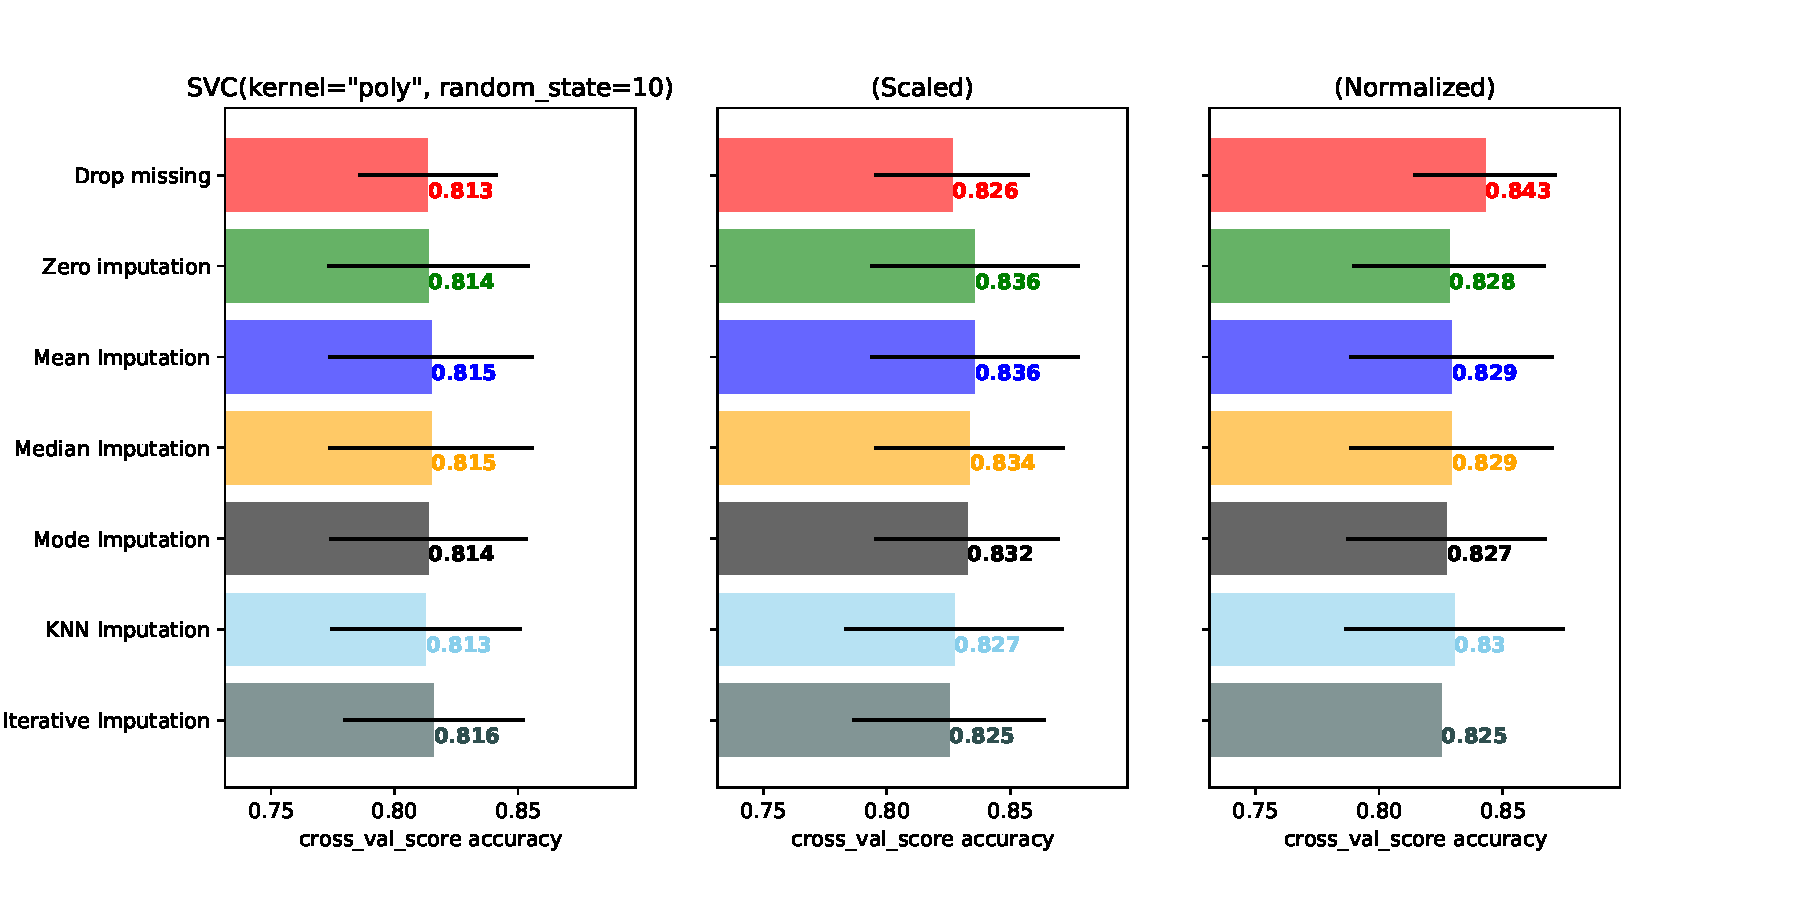
\includegraphics[width=\textwidth]{./code/figures_python/imputation_techniques/imputation_techniques_svc_poly_scaled_minmax.pdf}
\label{imputation-scaled-2}
\end{figure}

Finalmente, vemos que no se aprecia gran diferencia entre los tipos de imputaciones y los resultados obtenidos, incluso a veces obtenemos mejores resultados simplemente eliminando los valores perdidos, lo cuál suena la campana de que nuestros valores producen mucho "ruido", influye mucho más el tipo de escalado en nuestros datos.

En la práctica para este dataset, vamos a proceder siempre a estandarizar nuestros datos numéricos para los estimadores con los que vamos a trabajar debido a los resultados vistos en las figuras anteriores ya que solo beneficia o directamente no cambia nada. También trabajaremos  codificando nuestras variables categóricas con LabelEncoding o OneHotEncoding, después de estandarizar y codificar nuestros datos, procederemos a deshacernos de los valores perdidos o usaremos distintos tipos de imputación dependiendo de si la variable es numérica o categórica (por ejemplo, sustituyendo por la media para variables numéricas y por la moda para variables categóricas) estudiaremos estos resultados con más profundidad en el apartado siguiente de \textbf{[\nameref{chapter:cfg}]}

%%%%%%%%%%%%%%%%%%%%%%%%%%%%%%%%%%%%
\chapter*{Configuración de algoritmos}
\label{chapter:cfg}
\addcontentsline{toc}{chapter}{Configuración de algoritmos}  

En esta sección hablaremos un poco de varios algoritms probando distintas configuraciones y mostrando los resultados \footnote{El código para las configuraciones puede encontrarse en el jupyter notebook \textbf{estimators.ipynb} entregado en la carpeta de code}, se utilizarán tablas comparativas con los resultados del algoritmo con las distintas variaciones estudiadas. Para hallar la mejor combinación de parámetros posible se hará uso de GridSearchCV \cite{grid-search-cv}, el cuál utiliza validación cruzada internamente para la selección de parámetros. Se mostrará también Validation y Learning Curves para comentar el entrenamiento del modelo.

Como configuración por defecto utilizaremos la siguiente pipeline, probaremos distintas combinaciones de imputaciones como hemos comentando en la sección anterior y donde pone \textbf{LogisticRegression()} usaremos el estimador correspondiente, se tendrá en cuenta dos configuraciones iniciales, la de esta pipeline, y el drop missing utilizado anteriormente donde simplemente eliminamos todos los valores perdidos junto al estimador correspondiente.
\begin{figure}[h]
 \begin{lstlisting}
categorical_features = ['Shape']
categorical_transformer = Pipeline(
    [('imputer_cat', SimpleImputer()),
        ('onehot', OneHotEncoder(handle_unknown = 'ignore'))]
)
numeric_features = ['BI-RADS','Age', 'Margin', 'Density']
numeric_transformer = Pipeline(
    [('imputer_num', SimpleImputer()),
        ('scaler', StandardScaler())]
)
preprocessor = ColumnTransformer(
    [('cat', categorical_transformer, categorical_features),
        ('num', numeric_transformer, numeric_features)]
)
pipeline = Pipeline(
    [('pre', preprocessor), ('clf', LogisticRegression())]
)
 \end{lstlisting}
 \caption{Pipeline configuración por defecto}
 \end{figure}
 
 Dividiremos nuestro dataset en datos de entrenamiento y en datos de prueba en la proporción de 60-40
 
%%%%%%%%%%%%%%%%%%%%%%%%%%%%%%
\section*{LogisticRegression}
\addcontentsline{toc}{section}{LogisticRegression}  
La Regresión Logística es un método estadístico para predecir clases binarias. El resultado o variable objetivo es de naturaleza dicotómica. (solo hay dos clases posibles, en nuestro caso maligno codificado con 1 y benigno codificado con 0). Lleva el nombre de la función utilizada en el núcleo del método, función Sigmoide. Esta función es una curva en forma de S que puede tomar cualquier número de valor real y asignar a un valor entre 0 y 1. Si la curva va a infinito positivo la predicción se convertirá en 1, y si la curva pasa el infinito negativo, la predicción se convertirá en 0. Si la salida de la función Sigmoide es mayor que 0.5, podemos clasificar el resultado como 1 o SI, y si es menor que 0.5 podemos clasificarlo como 0 o NO. Por su parte si el resultado es 0.75, podemos decir en términos de probabilidad como, hay un 75\% de probabilidades de que el paciente sufra cáncer. Básicamente es una regresión lineal con una función de activación al final que nos sirve para predecir una clase u otra. Aplicando la función Sigmoide en la Regresión Lineal (una variable dependiente,Y, que queremos predecir y otras variables que son las independientes, que nos ayudan a predecir nuestra variable dependiente, $X_i$). La función de la Regresión Lineal ($ Y = \beta_0 + \beta_1X_1 + \beta_2X_2 + \dot{...} + \beta_nX_n  $) nos quedaría lo siguiente: $$\frac{1}{1+e^{-(\beta_0 + \beta_1X_1 + \beta_2X_2 + \dot{...} + \beta_nX_n)}}$$

Haremos un hyperparameter tuning con lo que nos proporciona la libreria de skelearn \cite{logistic-regression} entre los siguientes parámetros:
\begin{itemize}
	\item penalty (regularización, se especifica la norma, algunos algoritmos solo soportan unas, probaremos las normas ['l1', 'l2', 'elasticnet']
	\item C (para reducir el overfitting, cuanto más pequeño, mayor es la regularización, probaremos [100, 10, 1.0, 0.1, 0.01])
	\item solver (algoritmo encargado de resolver el problema de clasificiación, probaremos ['newton-cg', 'lbfgs', 'liblinear'])	
\end{itemize}


En la \textbf{Tabla[\ref{lr:inicial}]} mostramos los resultados de nuestra configuración por defecto usando la pipeline y sin preprocesamiento.

\begin{table}[h]
\begin{center}
  \begin{tabular}{|c|c|c|c|}
  \hline
    \multicolumn{4}{|c|}{\textbf{Puntuación configuración por defecto LogisticRegression}} \\  
     \hline
    \multicolumn{2}{|c|}{\textbf{pipeline}} & \multicolumn{2}{|c|}{\textbf{LogisticRegression()}}\\    
     \hline
   cross\_val\_score & std & cross\_val\_score & std  \\ 
    \hline
0.8304 & 0.0319 & 0.8193 & 0.0182  \\ 
\hline 
  \end{tabular}
  \end{center}
\caption{LogisticRegression - Inicial}
\label{lr:inicial}
\end{table}

Hacemos uso de GridSearchCV para encontrar la mejor combinación de parámetros junto a distintas estrategias de imputaciónes, mostramos los resultados ordenados por Accuracy en la tabla [\ref{lr:table}], debido a la longitud de la misma elegimos mostrar solo los resultados que alcanza un Accuracy como mínimo nuestro resultado inicial (0.83), también mostramos la \textbf{Fig. [\ref{lr:graph}]} donde mostramos resultados de los 3 distintos solvers mientras aumentamos el valor de nuestro regulador C. Vemos que la modificación de resultados proporciona resultados despreciables. Los resultados de newton y lbfgs ( Limited-memory Broyden–Fletcher–Goldfarb–Shanno Algorithm) son análogos ya que utilizan la misma matrix Hessiana pero aproximada, en nuestro caso parece ser equivalente. Parece ser que el factor de escoger nuestro regulador C es el que más condiciona a nuestra accuracy ya que vemos variedad de combinaciones con los otros parámetros que no hace cambiar el resultado.

\begin{table}[ht!]
\begin{center}
\resizebox{\textwidth}{!}{\begin{tabular}{rllllr}
\toprule
 clf\_\_C & clf\_\_penalty & clf\_\_solver & pre\_\_cat\_\_imputer\_cat\_\_strategy & pre\_\_num\_\_imputer\_num\_\_strategy &  Accuracy \\
\midrule
   0.01 &           l2 &   newton-cg &                          median &                          median &  0.841667 \\
   0.01 &           l2 &         sag &                          median &                          median &  0.841667 \\
   0.01 &           l2 &         sag &                   most\_frequent &                          median &  0.841667 \\
   0.01 &           l2 &         sag &                   most\_frequent &                            mean &  0.841667 \\
   0.01 &           l2 &        saga &                   most\_frequent &                            mean &  0.841667 \\
   0.01 &           l2 &        saga &                   most\_frequent &                          median &  0.841667 \\
   0.01 &           l2 &        saga &                          median &                            mean &  0.841667 \\
   0.01 &           l2 &        saga &                          median &                          median &  0.841667 \\
   0.01 &           l2 &       lbfgs &                          median &                          median &  0.841667 \\
   0.01 &           l2 &       lbfgs &                          median &                            mean &  0.841667 \\
   0.01 &           l2 &       lbfgs &                   most\_frequent &                          median &  0.841667 \\
   0.01 &           l2 &       lbfgs &                   most\_frequent &                            mean &  0.841667 \\
   0.01 &           l2 &   newton-cg &                          median &                            mean &  0.841667 \\
   0.01 &           l2 &   newton-cg &                   most\_frequent &                          median &  0.841667 \\
   0.01 &           l2 &   newton-cg &                   most\_frequent &                            mean &  0.841667 \\
   0.01 &           l2 &         sag &                          median &                            mean &  0.841667 \\
   0.10 &           l2 &   liblinear &                   most\_frequent &                            mean &  0.839583 \\
   0.10 &           l2 &   liblinear &                   most\_frequent &                          median &  0.839583 \\
   0.10 &           l2 &   liblinear &                          median &                            mean &  0.839583 \\
   0.10 &           l2 &   liblinear &                          median &                          median &  0.839583 \\
   0.10 &           l2 &       lbfgs &                          median &                          median &  0.835417 \\
   0.10 &           l2 &         sag &                   most\_frequent &                          median &  0.835417 \\
   0.10 &           l2 &        saga &                          median &                          median &  0.835417 \\
\bottomrule
\end{tabular}
}
\end{center}
\caption{LogisticRegression Combinations - Accuracy}
\label{lr:table}
\end{table}

\begin{figure}[ht!]
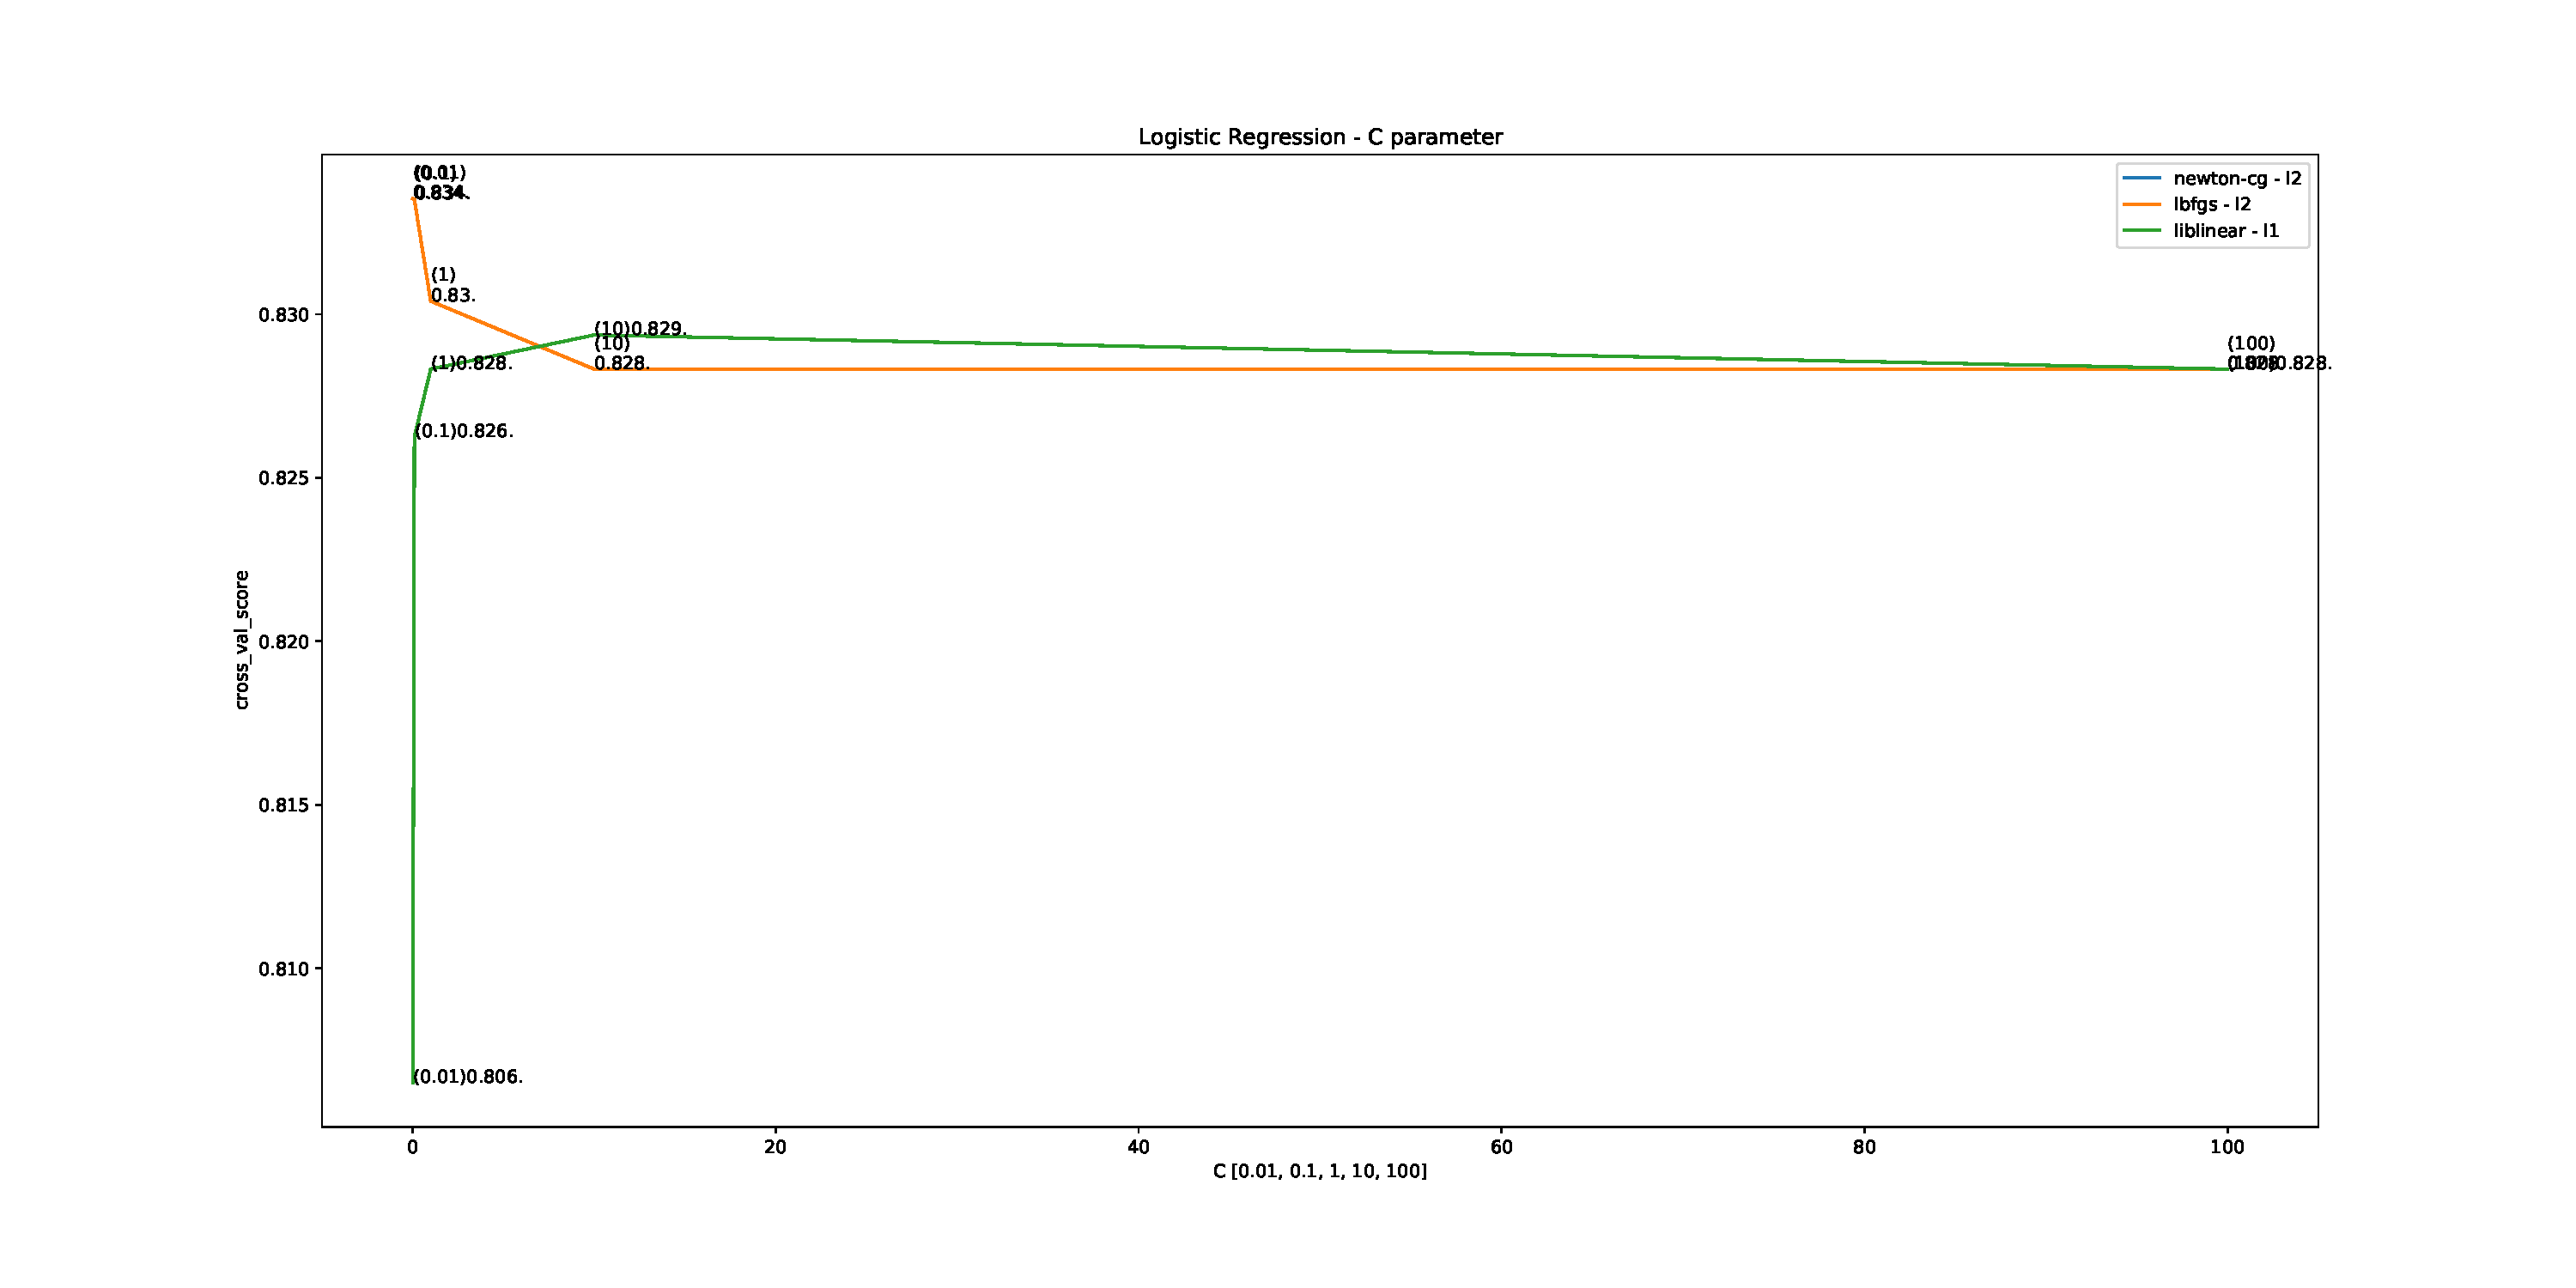
\includegraphics[width=\textwidth]{./code/figures_python/parameters/lr_graph.pdf}
\caption{Logistic Regression - Graph}
\label{lr:graph}
\end{figure}

Una vez obtenido nuestro modelo con la mejor combinación de parámetros, mostramos curvas de validación y de aprendizaje del mismo junto a una gráfica respecto a la estabilidad y el rendimiento en la \textbf{Fig. [\ref{lr:curves}]} . La curva de validación calcula las puntuaciones de un estimador con diferentes valores de un parámetro específico, mientras que la curva de aprendizaje determina cross-validated training y test scores para diferentes tamaños de conjuntos de entreno, es simplemente una utilidad para graficar los resultados.
En el caso de nuestra Validation Curve nos encontramos en situación de good fit, donde no se produce underfitting ni overfitting. En nuestra learning curve como las scores de cross val y de test convergen juntas a medida que se agregan más datos (como se muestra en la figura), entonces el modelo probablemente no se beneficiará de más datos.

\begin{figure}[ht!]
\begin{multicols}{2}
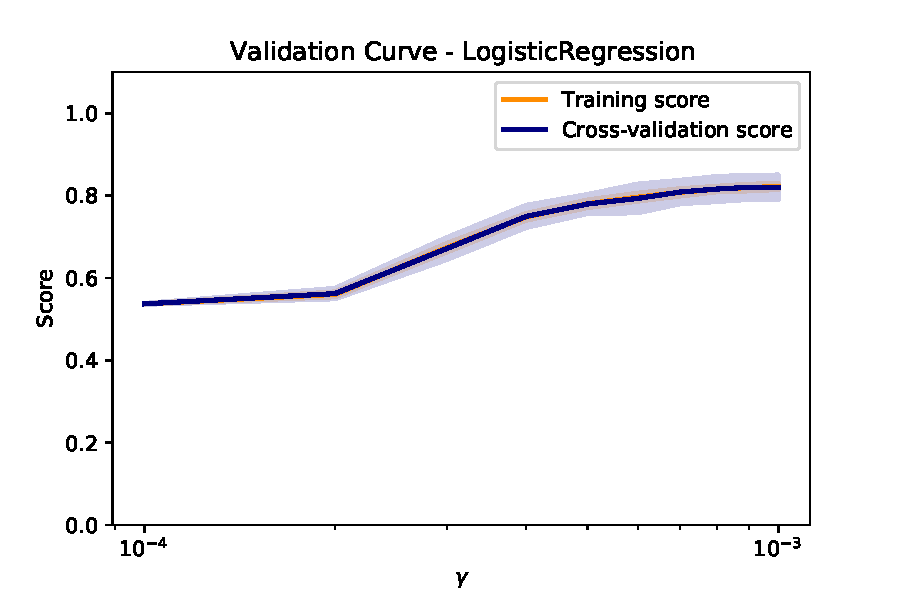
\includegraphics[width=8.5cm]{./code/figures_python/validation_curves/lr.pdf}%
\columnbreak
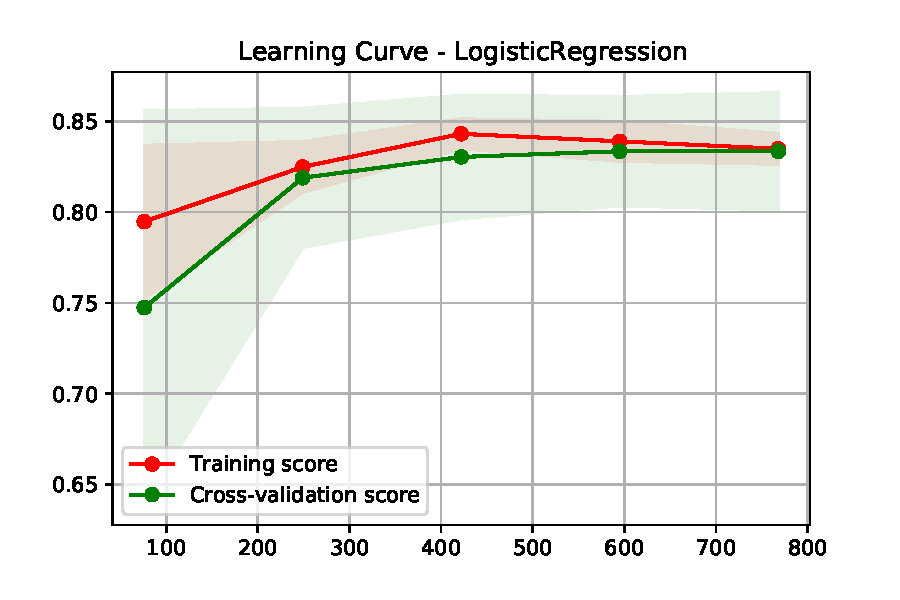
\includegraphics[width=8.5cm]{./code/figures_python/learning_curves/lr.pdf}%
\end{multicols}

\begin{multicols}{2}
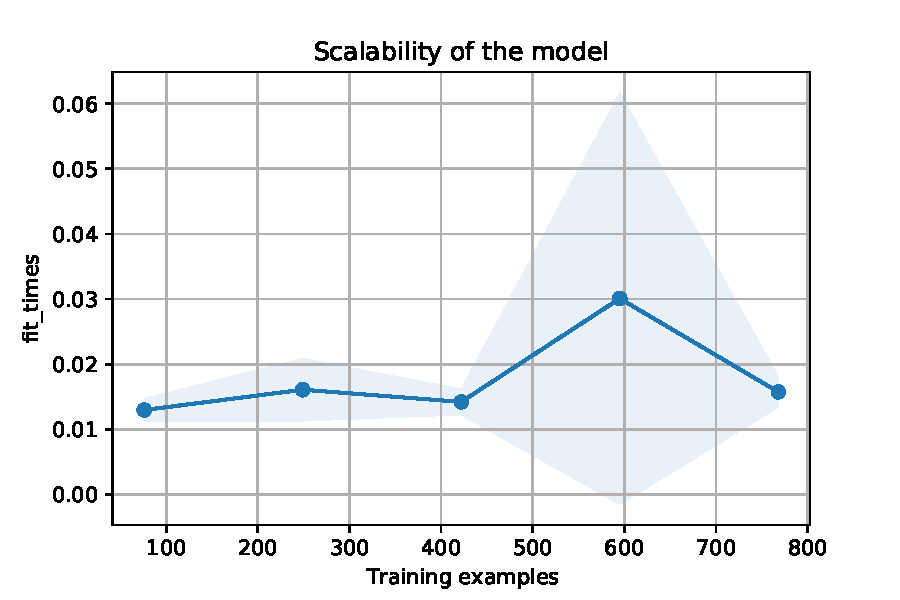
\includegraphics[width=8.5cm]{./code/figures_python/learning_curves/lr_scalability.pdf}%
\columnbreak
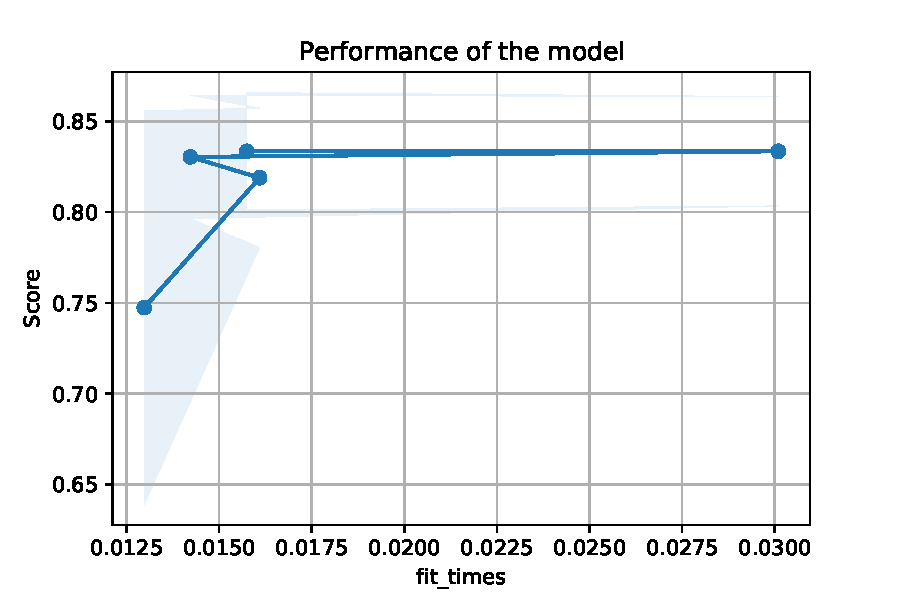
\includegraphics[width=8.5cm]{./code/figures_python/learning_curves/lr_performance.pdf}%
\end{multicols}
\caption{Logistic Regression - Curvas}
\label{lr:curves}
\end{figure}


%%%%%%%%%%%%%%%%%%%%%%%%%%%%%%
\section*{KNeighborsClassifier}
\addcontentsline{toc}{section}{KNeighborsClassifier}  
\label{section:knn}

KNeighborsClassifier es un algoritmo basado en instancia de tipo supervisado de Machine Learning. Sirve esencialmente para clasificar valores buscando los puntos de datos “más similares” (por cercanía) aprendidos en la etapa de entrenamiento y haciendo conjeturas de nuevos puntos basado en esa clasificación. Esto lo hace mediante el cálculo de la distancia entre el item a clasificar y el resto de items seleccionando los "k" elementos más cercanos, este parámetro k será en el que nos centremos en este caso. Destacamos la importancia de escalar nuestros datos para que estén en la misma escala debido al uso de distancias, limitaremos nuestro k a $25$ ya que un valor muy grande de nuestra k hace mucho sobreaprendizaje.

Haremos un hyperparameter tuning con lo que nos proporciona la libreria de skelearn \cite{knn} entre los siguientes parámetros:
\begin{itemize}
	\item n\_neighbors (nuestra "k" comentada anteriormente, default = 5)
	\item metrics (probaremos distintas métricas [euclidean, manhattan, chebyshev, default: minkowski])
\end{itemize}

En la tabla [\ref{knn:inicial}] mostramos los resultados de nuestra configuración por defecto usando la pipeline y sin preprocesamiento.

\begin{table}[h]
\begin{center}
  \begin{tabular}{|c|c|c|c|}
  \hline
    \multicolumn{4}{|c|}{\textbf{Puntuación configuración por defecto KNeighborsClassifier}} \\  
    \hline
    \multicolumn{2}{|c|}{\textbf{pipeline}} & \multicolumn{2}{|c|}{\textbf{KNeighborsClassifier()}}\\    
    \hline
   cross\_val\_score & std & cross\_val\_score & std  \\ 
   \hline
0.7971 & 0.027 & 0.8004 & 0.0214  \\ 
\hline
  \end{tabular}
  \end{center}
\caption{KNeighborsClassifier - Inicial}
\label{knn:inicial}
\end{table}

Hacemos uso otra vez de GridSearchCV para encontrar la mejor combinación de parámetros junto a distintas estrategias de imputaciónes, mostramos los resultados ordenados por Accuracy en la \textbf{Tabla. [\ref{knn:table}]}, debido a la longitud de la misma elegimos mostrar solo los resultados que alcanza un Accuracy considerable, vemos la importancia de escalar los valores antes de proceder con el estimador, StandardScaler() se encuentra siempre entre las combinaciones con mejores puntuaciones. El tipo de imputación elegida no es tan importante, pero vemos que la métrica de manhattan funciona ligeramente mejor en este conjunto de datos (sabemos por la asignatura de Análisis funcional que la métrica de Manhattan norma L1 puede ser preferible a otras métricas de norma L2 para el caso de ciertas dimensiones de datos).


\begin{table}[ht!]
\begin{center}
\resizebox{\textwidth}{!}{\begin{tabular}{lrlllr}
\toprule
clf\_\_metric &  clf\_\_n\_neighbors & pre\_\_cat\_\_imputer\_cat\_\_strategy & pre\_\_num\_\_imputer\_num\_\_strategy &  pre\_\_num\_\_scaler &  Accuracy \\
\midrule
  manhattan &                16 &                          median &                          median &  StandardScaler() &  0.836022 \\
  manhattan &                16 &                   most\_frequent &                            mean &  StandardScaler() &  0.836022 \\
  manhattan &                16 &                          median &                            mean &  StandardScaler() &  0.836022 \\
  manhattan &                16 &                   most\_frequent &                          median &  StandardScaler() &  0.836022 \\
  manhattan &                17 &                   most\_frequent &                            mean &  StandardScaler() &  0.833424 \\
  manhattan &                17 &                          median &                            mean &  StandardScaler() &  0.833424 \\
  manhattan &                18 &                   most\_frequent &                            mean &  StandardScaler() &  0.833390 \\
  manhattan &                18 &                   most\_frequent &                          median &  StandardScaler() &  0.833390 \\
  manhattan &                18 &                          median &                            mean &  StandardScaler() &  0.833390 \\
  manhattan &                18 &                          median &                          median &  StandardScaler() &  0.833390 \\
  manhattan &                19 &                          median &                            mean &  StandardScaler() &  0.833356 \\
  manhattan &                19 &                   most\_frequent &                            mean &  StandardScaler() &  0.833356 \\
  manhattan &                17 &                   most\_frequent &                          median &  StandardScaler() &  0.830793 \\
  manhattan &                17 &                          median &                          median &  StandardScaler() &  0.830793 \\
  manhattan &                15 &                          median &                          median &  StandardScaler() &  0.828195 \\
  euclidean &                17 &                   most\_frequent &                            mean &  StandardScaler() &  0.828195 \\
  manhattan &                15 &                   most\_frequent &                          median &  StandardScaler() &  0.828195 \\
  euclidean &                17 &                          median &                            mean &  StandardScaler() &  0.828195 \\
  manhattan &                19 &                          median &                          median &  StandardScaler() &  0.828161 \\
  manhattan &                19 &                   most\_frequent &                          median &  StandardScaler() &  0.828161 \\
  euclidean &                16 &                   most\_frequent &                            mean &  StandardScaler() &  0.825598 \\
  euclidean &                17 &                   most\_frequent &                          median &  StandardScaler() &  0.825598 \\
  euclidean &                16 &                          median &                          median &  StandardScaler() &  0.825598 \\
  euclidean &                17 &                          median &                          median &  StandardScaler() &  0.825598 \\
  euclidean &                16 &                          median &                            mean &  StandardScaler() &  0.825598 \\
  euclidean &                16 &                   most\_frequent &                          median &  StandardScaler() &  0.825598 \\
  euclidean &                12 &                          median &                            mean &  StandardScaler() &  0.823035 \\
  euclidean &                12 &                   most\_frequent &                          median &  StandardScaler() &  0.823035 \\
  euclidean &                12 &                          median &                          median &  StandardScaler() &  0.823035 \\
  euclidean &                12 &                   most\_frequent &                            mean &  StandardScaler() &  0.823035 \\
\bottomrule
\end{tabular}
}
\end{center}
\caption{KNeighborsClassifier - Accuracy}
\label{knn:table}
\end{table}

\begin{figure}[h!]
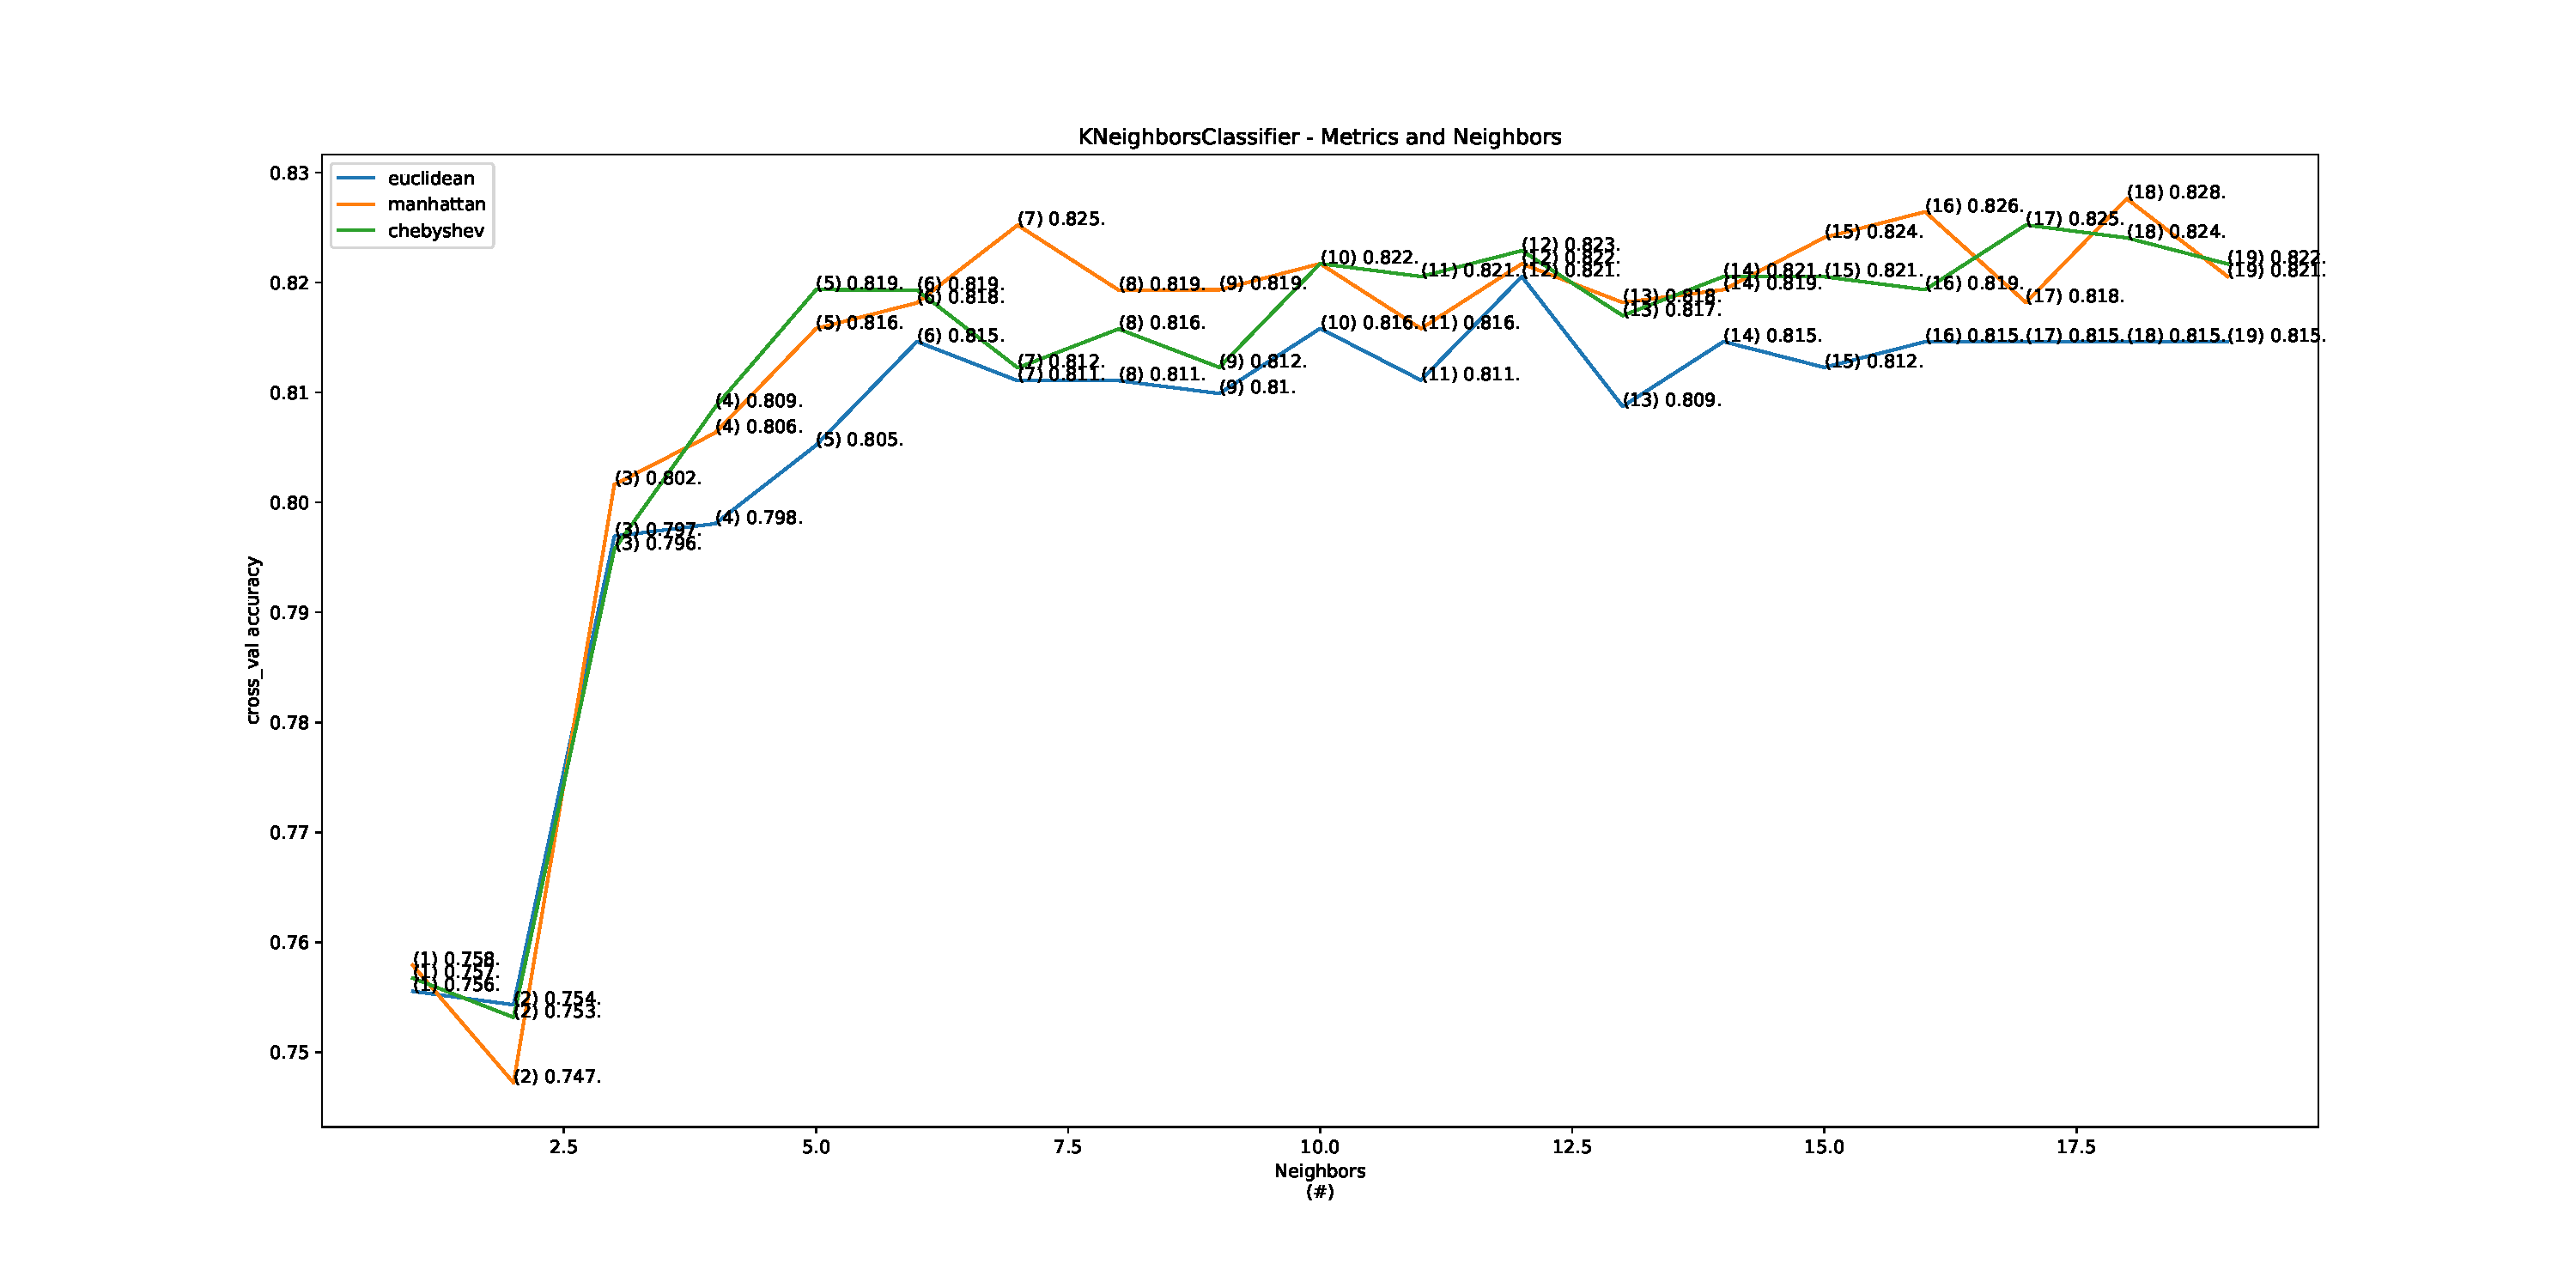
\includegraphics[width=\textwidth]{./code/figures_python/parameters/knn_graph.pdf}
\caption{KNeighborsClassifier - Graph}
\label{knn:graph}
\end{figure}

Una vez obtenido nuestro modelo con la mejor combinación de parámetros, mostramos curvas de validación y de aprendizaje del mismo junto a una gráfica respecto a la estabilidad y el rendimiento en la \textbf{Fig. [\ref{knn:curves}]}. El modelo de k vecinos más cercanos (kNN) se usa comúnmente cuando la similitud es importante para la interpretación del modelo. Elegir k es difícil, cuanto mayor es k, más datos se incluyen en una clasificación, creando topologías de decisión más complejas, mientras que cuanto menor es k, más simple es el modelo y menos se puede generalizar. Usar una curva de validación es una excelente estrategia para elegir k, en nuestro caso, todo lo que podemos ver es una variabilidad decreciente en las puntuaciones de validación cruzada.
 Esta curva de validación plantea dos posibilidades: primero, que no tenemos el rango correcto para encontrar el mejor k y necesitamos expandir nuestra búsqueda a valores más grandes. La segunda es que otros hiperparámetros (como la ponderación uniforme o basada en la distancia, o incluso la elección de la métrica) pueden tener más influencia en el modelo predeterminado que k por sí mismo, aunque viendo el gráfico de la figura \textbf{Fig.[\ref{knn:graph}]} la diferencia no es muy apreciable.

\begin{figure}[ht!]
\begin{multicols}{2}
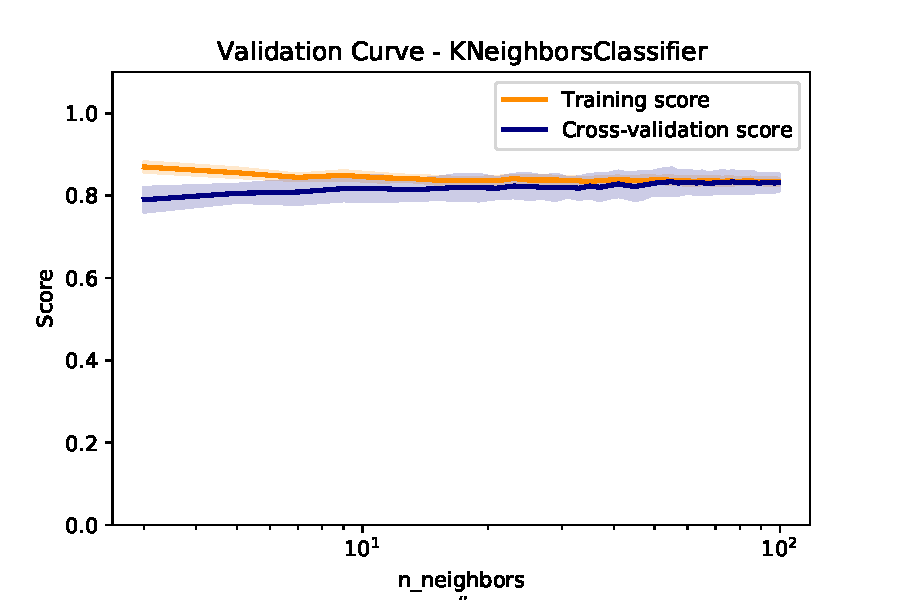
\includegraphics[width=8.5cm]{./code/figures_python/validation_curves/knn.pdf}%
\columnbreak
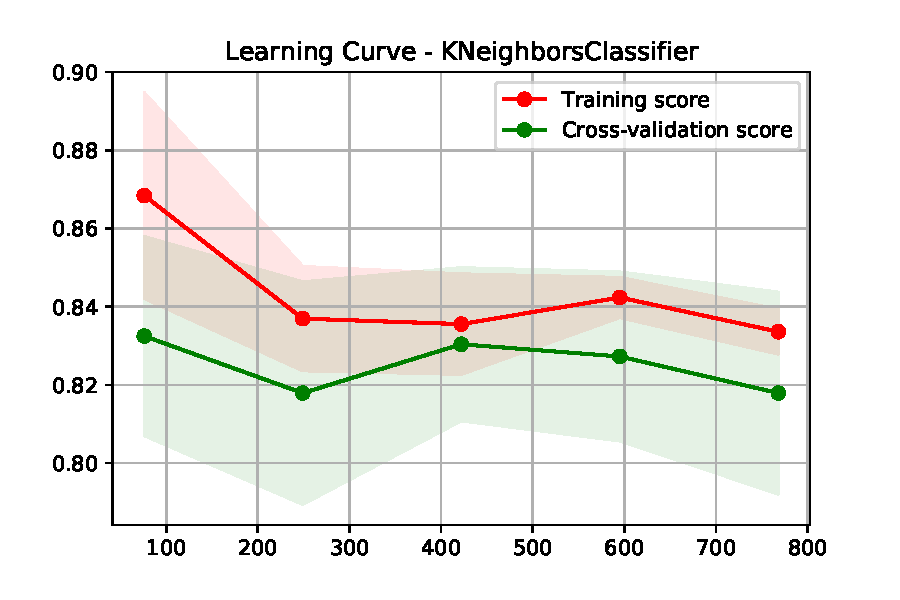
\includegraphics[width=8.5cm]{./code/figures_python/learning_curves/knn.pdf}%
\end{multicols}

\begin{multicols}{2}
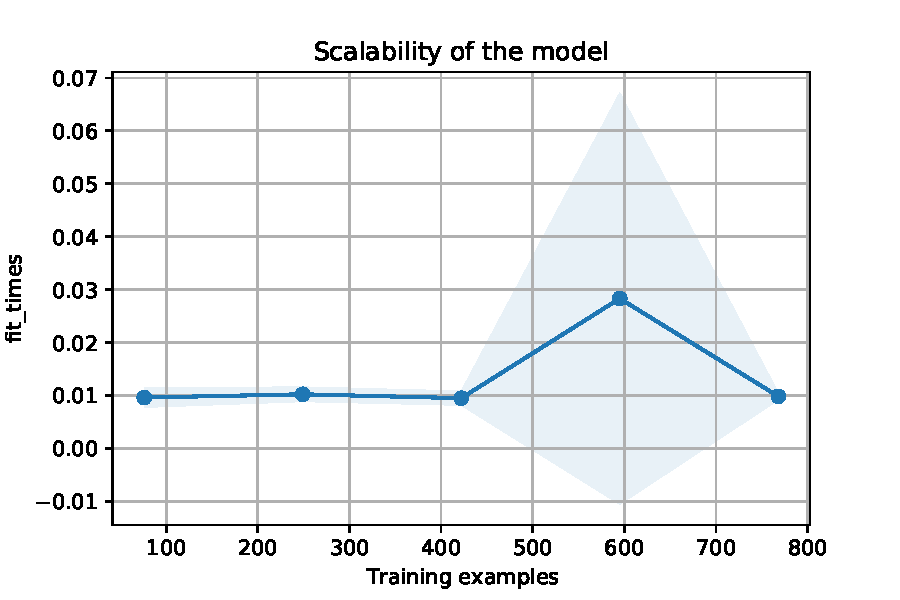
\includegraphics[width=8.5cm]{./code/figures_python/learning_curves/knn_scalability.pdf}%
\columnbreak
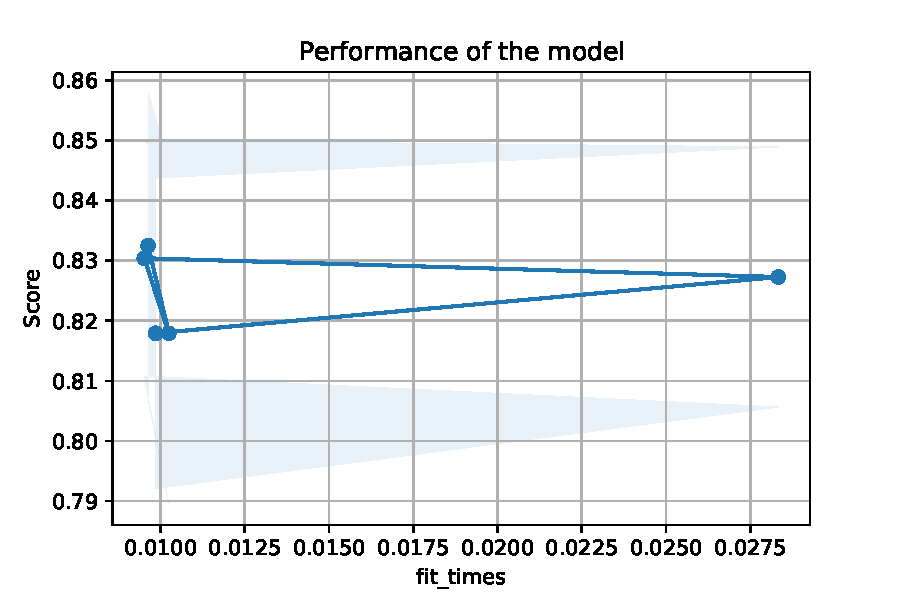
\includegraphics[width=8.5cm]{./code/figures_python/learning_curves/knn_performance.pdf}%
\end{multicols}
\caption{KNeighborsClassifier - Curvas}
\label{knn:curves}
\end{figure}

%%%%%%%%%%%%%%%%%%%%%%%%%%%%%%
\section*{Support Vector Machines}
\addcontentsline{toc}{section}{Support Vector Machines}  

Una \textbf{SVM} (support vector machine) es un modelo de aprendizaje que se fundamenta en la Teoría de Aprendizaje Estadístico. La idea básica es encontrar un hiperplano canónico que maximice el margen del conjunto de datos de entrenamiento( nos garantiza una buena capacidad de generalización). Estos métodos explotan la información que proporciona el producto interno (escalar) entre los datos disponibles. Se busca el mejor hiperplano para separar las diferentes clases maximizando la distancia entre los puntos de muestra y el hiperplano, para ello se hace uso de funciones kernel (producto interno de dos elementos en algún espacio de características inducido) lo que nos da lugar a distintos tipos de SVM\footnote{Aunque entre los estimadores SVM también se encuentra NuSVC y LinearSVC, vamos a centrarnos en distintos tips de función para SVC ya que NuSVC en lugar de utilizar el parámetro C, utiliza el parámetro nu que controla el número de vectores de soporte y LinearSVC es semejante a SVC con el parámetro kernel="linear"}. Destacaremos algunos parámetros con lo que nos proporciona la libreria de skelearn \cite{svm}:

\begin{itemize}
	\item C (para reducir el overfitting, cuanto más pequeño, mayor es la regularización, probaremos [100, 10, 1.0, 0.1, 0.01])
	\item kernel (especifíca el tipo de hiperplano usado para separar los datos, tenemos lineales y no lineales probaremos ['linear', 'poly', 'rbf', 'sigmoid', 'precomputed'], default=’rbf’)
	\item $\gamma$,gamma (para hiperplanos no lineales, cuanto mayor sea el valor de gamma, intentará ajustarse exactamente al conjunto de datos de entrenamiento)
\end{itemize}

En la \textbf{Tabla.[\ref{svc:inicial}]} mostramos los resultados de nuestra configuración por defecto usando la pipeline y sin preprocesamiento.

\begin{table}[h]
\begin{center}
  \begin{tabular}{|c|c|c|c|}
  \hline
    \multicolumn{4}{|c|}{\textbf{Puntuación configuración por defecto SVC}} \\  
    \hline
    \multicolumn{2}{|c|}{\textbf{pipeline}} & \multicolumn{2}{|c|}{\textbf{SVC()}}\\    
    \hline
   cross\_val\_score & std & cross\_val\_score & std  \\ 
   \hline
0.8272 & 0.04 & 0.7816 & 0.023  \\ 
\hline
  \end{tabular}
  \end{center}
\caption{SVC - Inicial}
\label{svc:inicial}
\end{table}

Hacemos uso otra vez de GridSearchCV para encontrar la mejor combinación de parámetros junto a distintas estrategias de imputaciónes, mostramos los resultados ordenados por Accuracy en la \textbf{Tabla.[\ref{svc:table}]}, debido a la longitud de la misma elegimos mostrar solo los resultados que alcanza un Accuracy considerable. Como en el caso de \textbf{KNeighborsClassifier}, destacamos la importancia de escalar los datos, SVM intenta maximizar la distancia entre el plano de separación y los support vectors. Si una característica (es decir, una dimensión en este espacio) tiene valores muy grandes, dominará las otras características al calcular la distancia.

Si la train score y la score de la validación cruzada son bajas, el estimador no se ajustará correctamente. Si la puntuación de entrenamiento es alta y la puntuación de validación es baja, el estimador está sobreajustado y, por lo demás, está funcionando muy bien. Por lo general, no es posible obtener una puntuación de entrenamiento baja y una puntuación de validación alta. Los tres casos se pueden encontrar en el nuestra curva de validación de la \textbf{Fig.[\ref{svc:curves}]}, donde variamos el parámetro $\gamma$ de una SVM en nuestro conjunto de datos. Para valores muy bajos de gamma, se puede ver que tanto la puntuación de entrenamiento como la validation score son bajas. A esto se le llama \textbf{underfit}. Los valores medios de gamma darán como resultado valores altos para ambas puntuaciones, es decir, el clasificador se está desempeñando bastante bien. Si la gamma es demasiado alta, el clasificador hará \textbf{overfitting}, lo que significa que la puntuación de entrenamiento es buena pero la validation score es mala. Para la Learning Curve como nuestras rectas no convergen el modelo se beneficiará de más datos.

\begin{table}[ht!]
\begin{center}
\resizebox{\textwidth}{!}{
\begin{tabular}{rlllllr}
\toprule
 clf\_\_C & clf\_\_gamma & clf\_\_kernel & pre\_\_cat\_\_imputer\_cat\_\_strategy & pre\_\_num\_\_imputer\_num\_\_strategy &  pre\_\_num\_\_scaler &  Accuracy \\
\midrule
   1.00 &       auto &         rbf &                   most\_frequent &                            mean &  StandardScaler() &  0.833356 \\
   1.00 &       auto &         rbf &                          median &                            mean &  StandardScaler() &  0.833356 \\
   1.00 &       auto &         rbf &                          median &                          median &  StandardScaler() &  0.830725 \\
   1.00 &       auto &         rbf &                   most\_frequent &                          median &  StandardScaler() &  0.830725 \\
   1.00 &      scale &         rbf &                   most\_frequent &                            mean &  StandardScaler() &  0.820335 \\
   1.00 &      scale &         rbf &                   most\_frequent &                          median &  StandardScaler() &  0.820335 \\
   1.00 &      scale &         rbf &                          median &                            mean &  StandardScaler() &  0.820335 \\
   1.00 &      scale &         rbf &                          median &                          median &  StandardScaler() &  0.820335 \\
   0.01 &      scale &     sigmoid &                   most\_frequent &                            mean &  StandardScaler() &  0.820335 \\
   0.01 &      scale &     sigmoid &                          median &                            mean &  StandardScaler() &  0.820335 \\
  10.00 &       auto &         rbf &                          median &                          median &  StandardScaler() &  0.820301 \\
   0.01 &      scale &     sigmoid &                   most\_frequent &                          median &  StandardScaler() &  0.820301 \\
   0.01 &      scale &     sigmoid &                          median &                          median &  StandardScaler() &  0.820301 \\
  10.00 &       auto &         rbf &                          median &                            mean &  StandardScaler() &  0.820301 \\
  10.00 &       auto &         rbf &                   most\_frequent &                          median &  StandardScaler() &  0.820301 \\
  10.00 &       auto &         rbf &                   most\_frequent &                            mean &  StandardScaler() &  0.820301 \\
  10.00 &      scale &        poly &                   most\_frequent &                          median &    MinMaxScaler() &  0.817703 \\
\bottomrule
\end{tabular}
}
\end{center}
\caption{SVC - Accuracy}
\label{svc:table}
\end{table}

\begin{figure}[ht!]
\begin{multicols}{2}
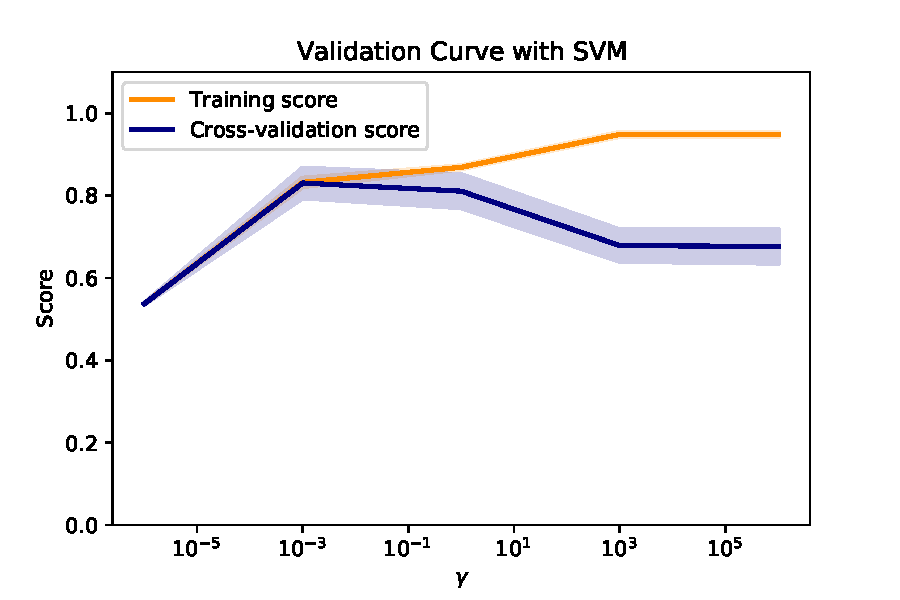
\includegraphics[width=8.5cm]{./code/figures_python/validation_curves/svc.pdf}%
\columnbreak
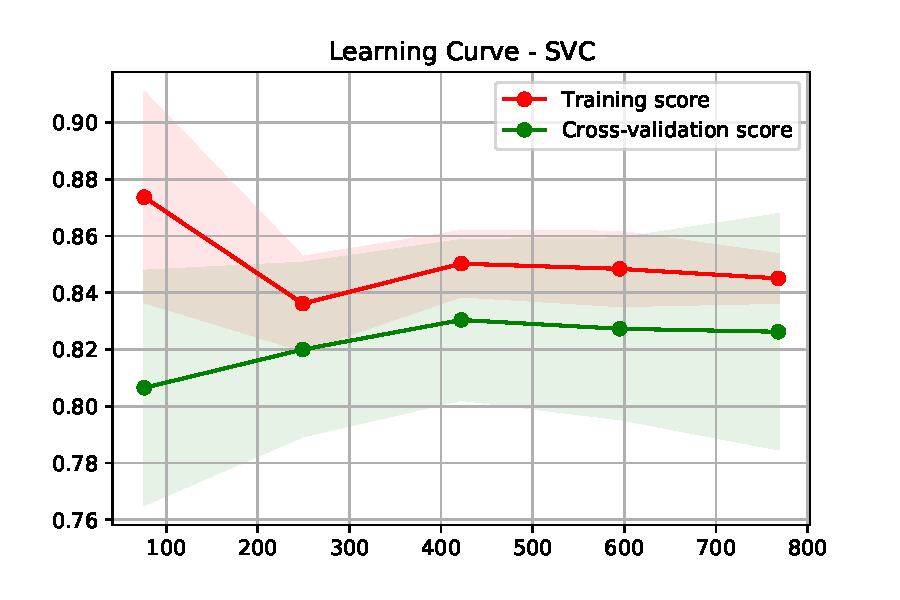
\includegraphics[width=8.5cm]{./code/figures_python/learning_curves/svc.pdf}%
\end{multicols}

\begin{multicols}{2}
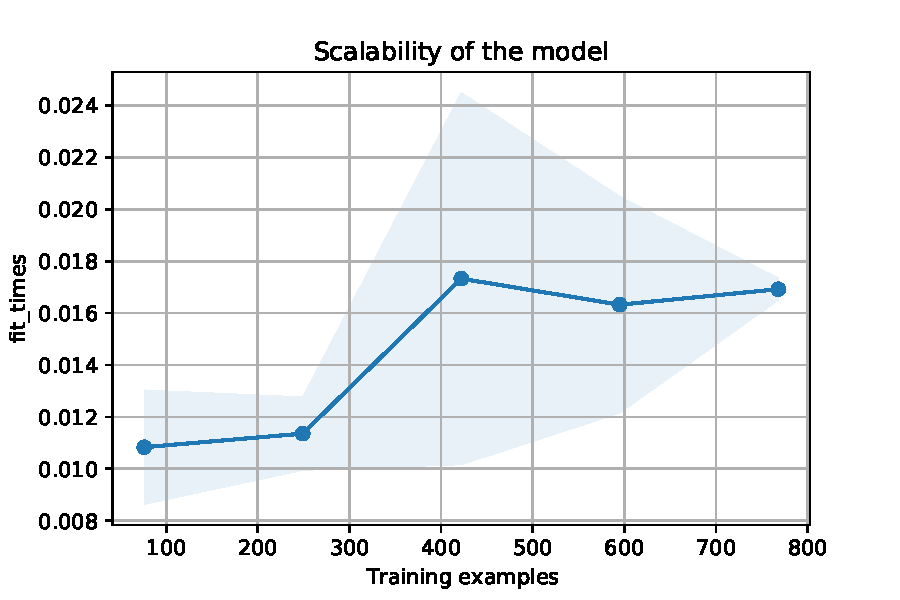
\includegraphics[width=8.5cm]{./code/figures_python/learning_curves/svc_scalability.pdf}%
\columnbreak
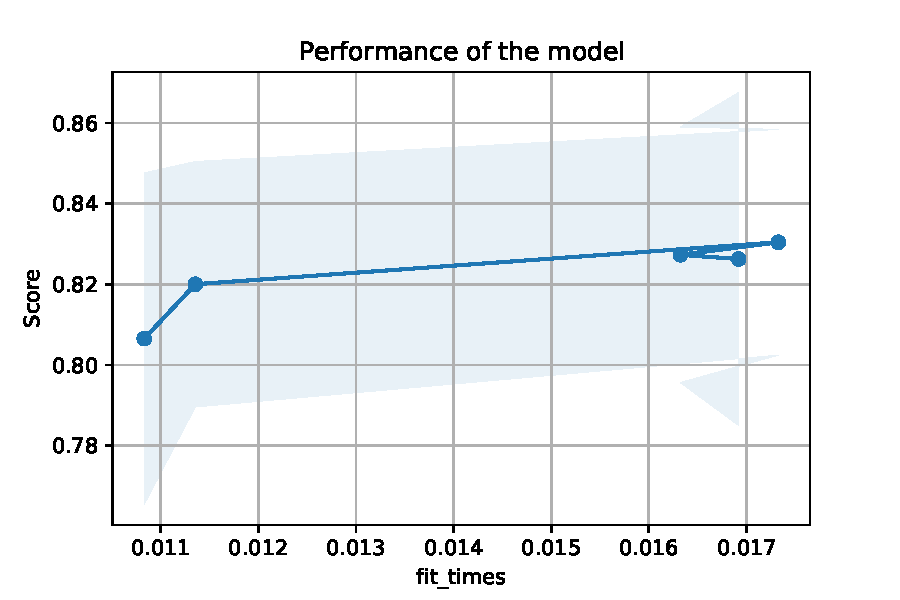
\includegraphics[width=8.5cm]{./code/figures_python/learning_curves/svc_performance.pdf}%
\end{multicols}
\caption{SVC - Curvas}
\label{svc:curves}
\end{figure}


\section*{Ensemble Clasiffiers}
\addcontentsline{toc}{section}{Ensemble Clasiffiers}  
Los \textbf{Ensemble Classiffiers}, combinan varios árboles de decisión para producir un mejor rendimiento predictivo que utilizando un solo árbol de decisión. El principio fundamental detrás de este tipo de estimadores es que un grupo de estimadores débiles se unen para formar uno fuerte. Hay varias técnicas para desarrollar este tipo de árboles, tenemos  Bagging (\textbf{B}oostrap \textbf{agg}regat\textbf{ing}) que se usa para combinar múltiples predictores/clasificadores y \textbf{Boosting}, escogemos un algoritmo de cada tipo (\textbf{RandomForestClassifier} y \textbf{GradientBoostingClassifier})

\subsection*{Random Forest}
\addcontentsline{toc}{subsection}{Random Forest}  
\textbf{Bagging} se utiliza cuando nuestro objetivo es reducir la varianza de un árbol de decisiones. Aquí la idea es crear varios subconjuntos de datos a partir de la muestra de entrenamiento elegida al azar con reemplazo. Ahora, cada colección de datos de subconjuntos se utiliza para entrenar sus árboles de decisión. Como resultado, terminamos con un conjunto de diferentes modelos. Se utiliza el promedio de todas las predicciones de diferentes árboles, que es más robusto que un solo árbol de decisión. 

Random Forest es una extensión del Bagging. Toma un paso adicional donde, además de tomar el subconjunto aleatorio de datos, también toma la selección aleatoria de características en lugar de usar todas las características para hacer crecer árboles. Cuando tienes muchos árboles aleatorios. Por eso se llama Random Forest!

Destacaremos estos parámetros que nos proporciona la libreria de skelearn \cite{rfc}:
        
\begin{itemize}
	\item n\_estimators (número de árboles, probaremos  [10, 100, 500])
	\item max\_depth (máxima profundidad del árbol, probaremos de 0 a 4)
\end{itemize}

En la \textbf{Tabla [\ref{rfc:inicial}]} mostramos los resultados de nuestra configuración por defecto usando la pipeline y sin preprocesamiento.

\begin{table}[h]
\begin{center}
  \begin{tabular}{|c|c|c|c|}
  \hline
    \multicolumn{4}{|c|}{\textbf{Puntuación configuración por defecto RandomForestClassifier}} \\  
    \hline
    \multicolumn{2}{|c|}{\textbf{pipeline}} & \multicolumn{2}{|c|}{\textbf{RandomForestClassifier()}}\\    
    \hline
   cross\_val\_score & std & cross\_val\_score & std  \\ 
   \hline
0.797 & 0.0316 & 0.785 & 0.03  \\ 
\hline
  \end{tabular}
  \end{center}
\caption{RandomForestClassifier - Inicial}
\label{rfc:inicial}
\end{table}

Algunas ventajas de usar RandomForest es que maneja muy bien datos de mayor dimensionalidad y los valores perdidos (mantiene la precisión de los datos perdidos) pero lo malo es que dado que la predicción final se basa en las predicciones medias de los árboles de subconjuntos, no proporcionará valores precisos para el modelo de regresión. De nuevo hacemos uso de GridSearchCV junto a curvas de validación y aprendizaje para ver como se comporta el estimador con la mejor combinación de parámetros comentados. En la tabla [\ref{rfc:table}] vemos las comparaciones de parámetros.


\begin{table}[ht!]
\begin{center}
\resizebox{\textwidth}{!}{
\begin{tabular}{rrllr}
\toprule
 clf\_\_max\_depth &  clf\_\_n\_estimators & pre\_\_cat\_\_imputer\_cat\_\_strategy & pre\_\_num\_\_imputer\_num\_\_strategy &  Accuracy \\
\midrule
              1 &                100 &                   most\_frequent &                          median &  0.833333 \\
              1 &                100 &                          median &                          median &  0.833333 \\
              3 &                100 &                          median &                          median &  0.833333 \\
              3 &                100 &                   most\_frequent &                          median &  0.833333 \\
              3 &                 10 &                          median &                          median &  0.833333 \\
              3 &                 10 &                   most\_frequent &                          median &  0.833333 \\
              1 &                 10 &                          median &                          median &  0.833333 \\
              1 &                 10 &                   most\_frequent &                          median &  0.833333 \\
              3 &                500 &                          median &                          median &  0.831250 \\
              2 &                100 &                   most\_frequent &                          median &  0.831250 \\
              3 &                500 &                          median &                            mean &  0.831250 \\
              3 &                500 &                   most\_frequent &                          median &  0.831250 \\
              3 &                500 &                   most\_frequent &                            mean &  0.831250 \\
              3 &                 10 &                          median &                            mean &  0.831250 \\
              3 &                 10 &                   most\_frequent &                            mean &  0.831250 \\
              2 &                100 &                          median &                          median &  0.831250 \\
              1 &                 10 &                   most\_frequent &                            mean &  0.829167 \\
              1 &                 10 &                          median &                            mean &  0.829167 \\
              3 &                100 &                   most\_frequent &                            mean &  0.829167 \\
              2 &                500 &                   most\_frequent &                          median &  0.829167 \\
              2 &                500 &                          median &                          median &  0.829167 \\
              3 &                100 &                          median &                            mean &  0.829167 \\
              1 &                500 &                          median &                          median &  0.827083 \\
\bottomrule
\end{tabular}
}
\end{center}
\caption{RFC - Accuracy}
\label{rfc:table}
\end{table}

Los Random Forest se sobreajustan cuanto más profundos son porque en cada nivel del árbol las particiones se ocupan de un subconjunto más pequeño de datos. Una forma de lidiar con este proceso de sobreajuste es limitar la profundidad del árbol. La curva de validación explora la relación del parámetro "max\_depth" usando cross\_val\_score con 5 validaciones cruzadas divididas aleatoriamente. 


Podemos ver en la \textbf{Fig.[\ref{rfc:curves}]} que en un límite de profundidad queda muy por debajo del modelo en este conjunto de datos porque la puntuación de entrenamiento y la puntuación de la prueba suben juntas en este rango de parámetros, y debido a la alta variabilidad de la validación cruzada en la prueba. Después de cierta profundidad, los scores de entrenamiento y de prueba divergen, esto se debe a que los árboles más profundos están comenzando a sobreajustarse a los datos de entrenamiento, lo que no permite generalizar el modelo. Sin embargo, debido a que la puntuación de validación cruzada no necesariamente disminuye, el modelo no sufre de un alto error debido a la varianza. También adjuntamos una gráfica en la \textbf{Fig.[\ref{rfc:graph}]} donde comparamos el aumento de estimadores entre árboles de distinta profundidad.

\begin{figure}[h!]
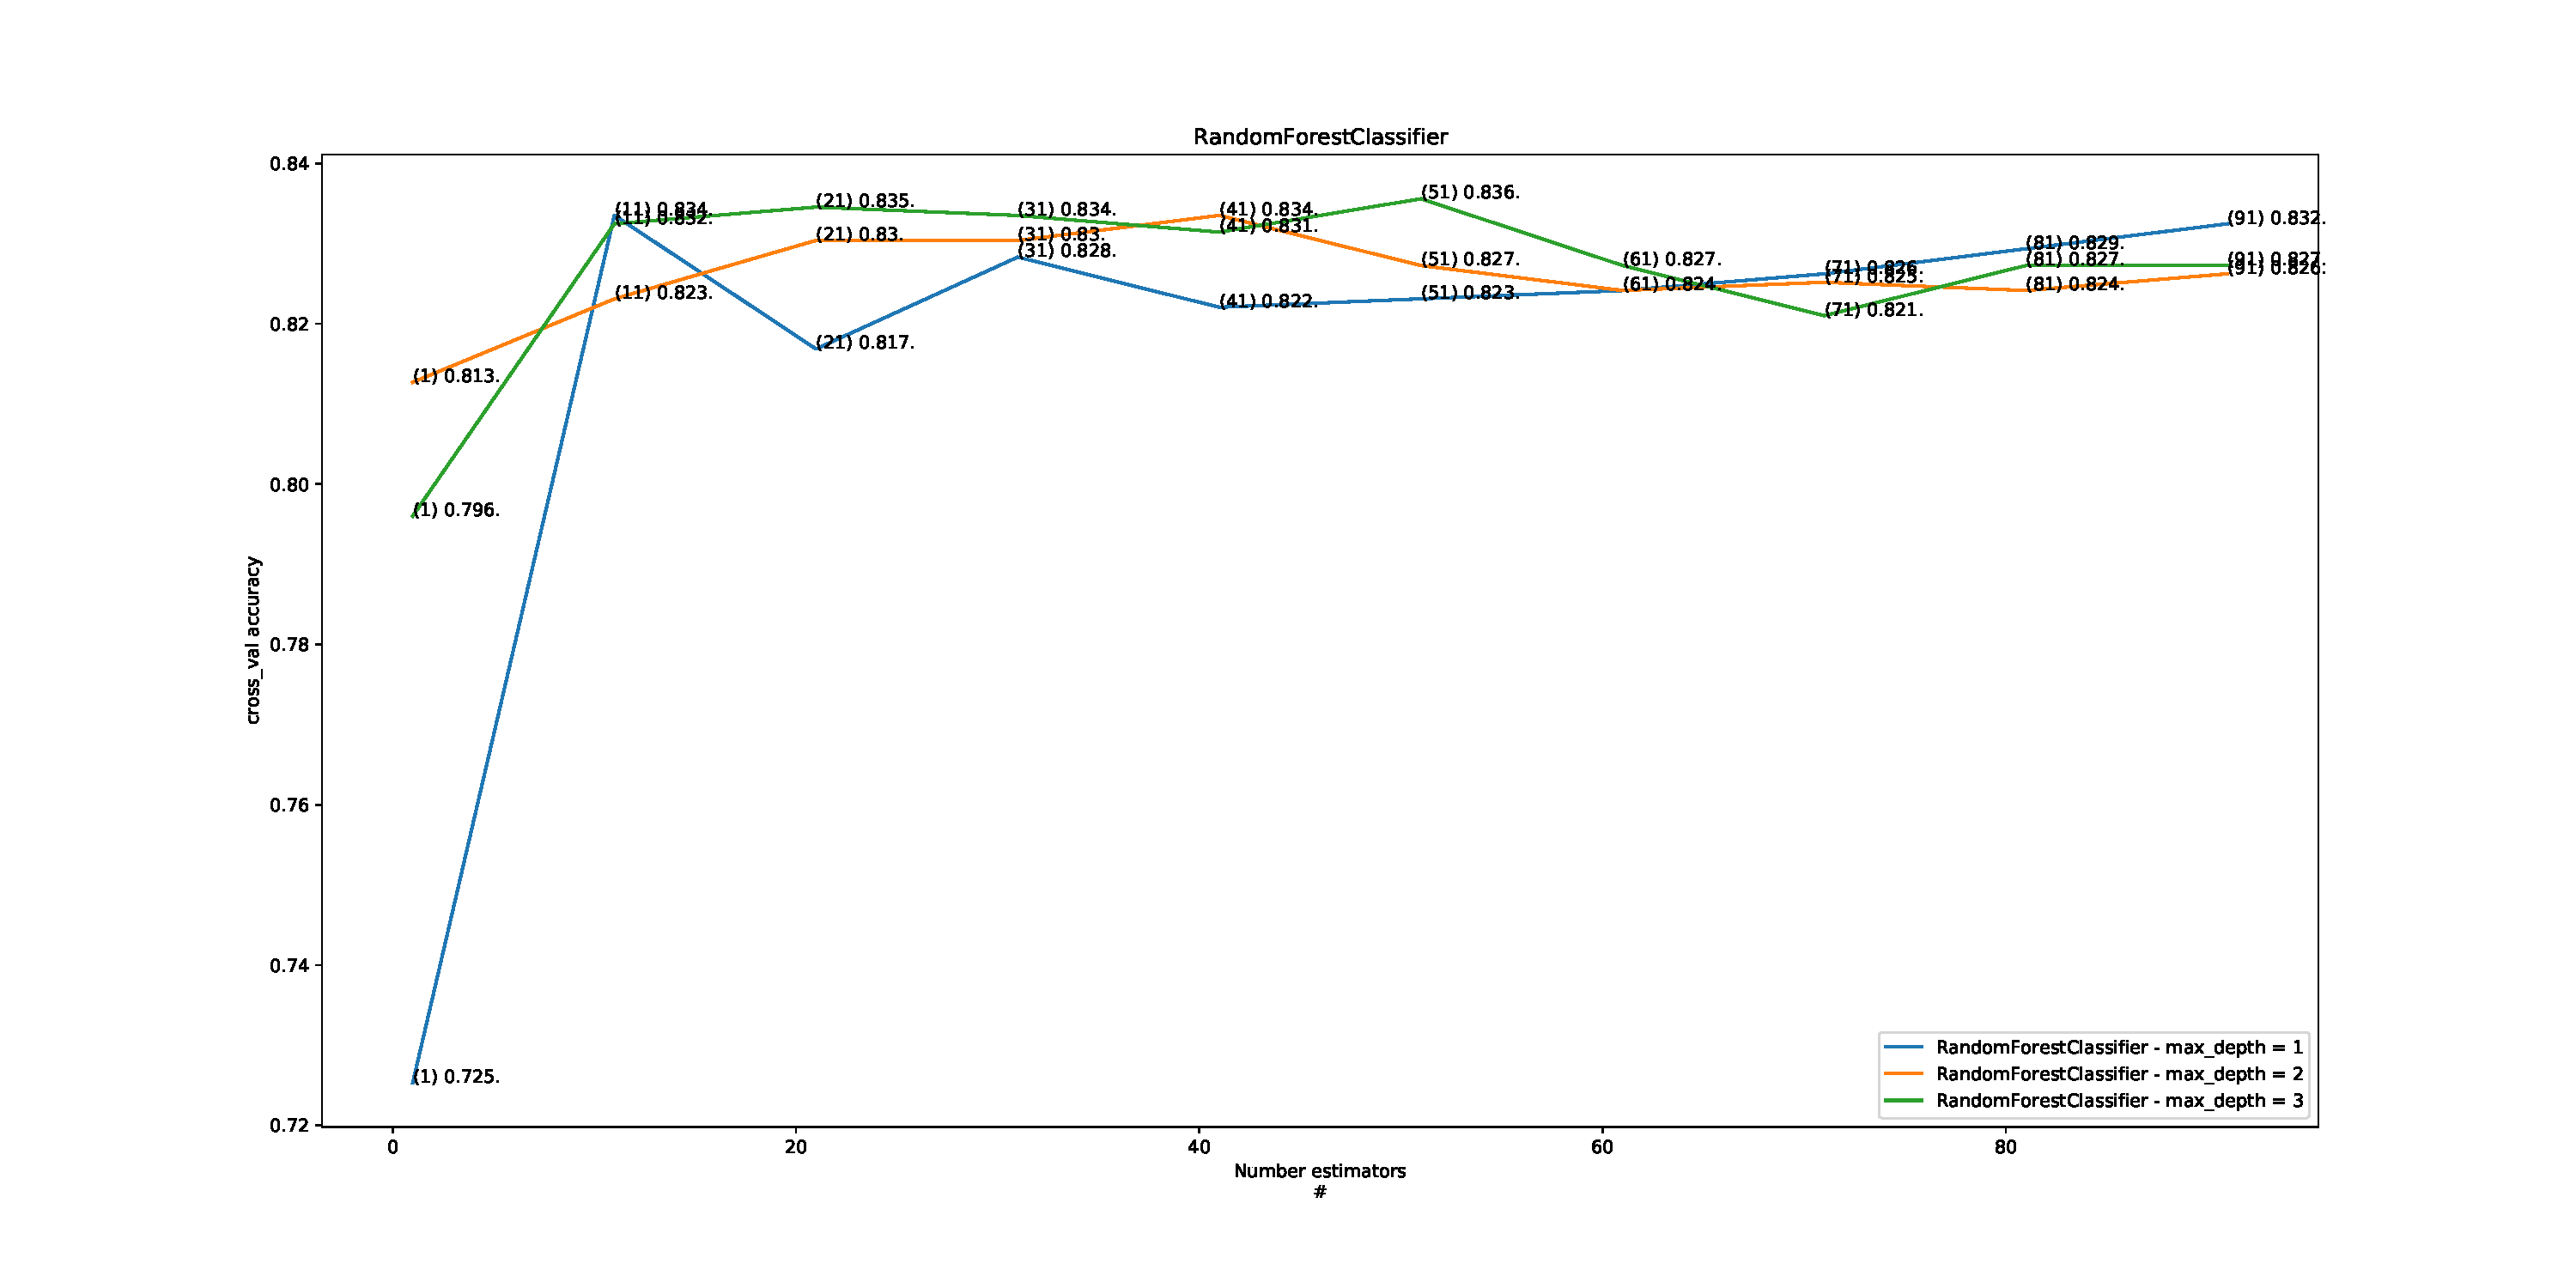
\includegraphics[width=\textwidth]{./code/figures_python/parameters/rfc_graph.pdf}
\caption{RFC - Graph}
\label{rfc:graph}
\end{figure}


\begin{figure}[ht!]
\begin{multicols}{2}
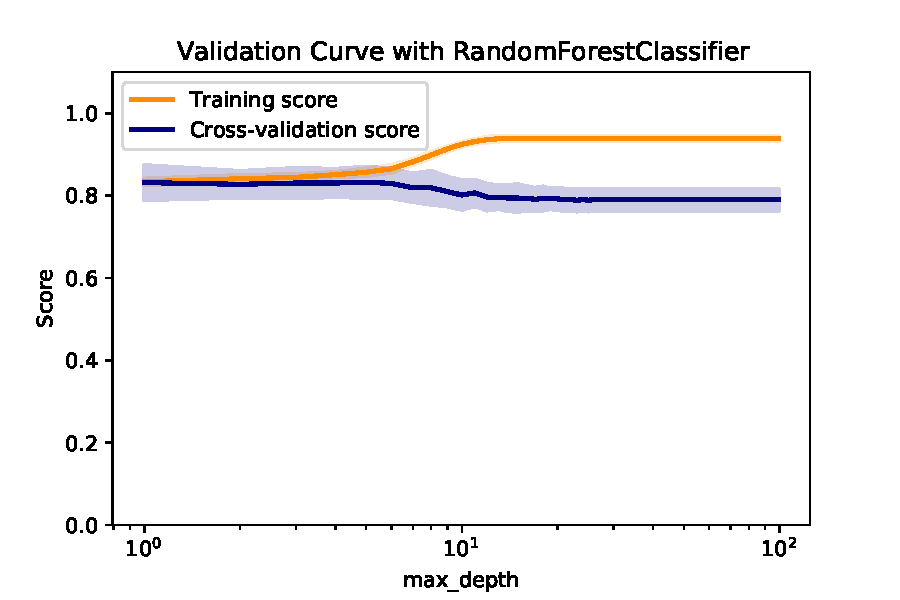
\includegraphics[width=8.5cm]{./code/figures_python/validation_curves/rfc.pdf}%
\columnbreak
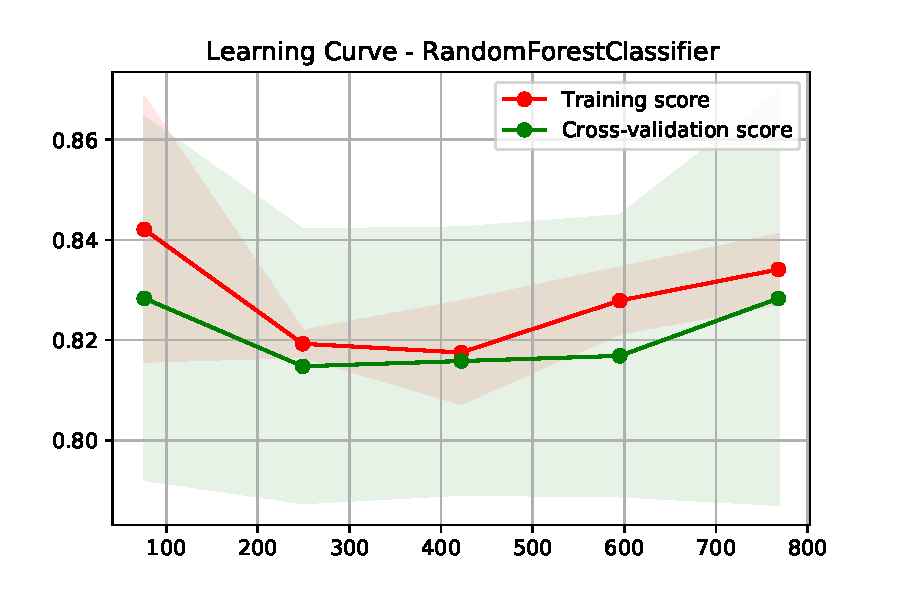
\includegraphics[width=8.5cm]{./code/figures_python/learning_curves/rfc.pdf}%
\end{multicols}

\begin{multicols}{2}
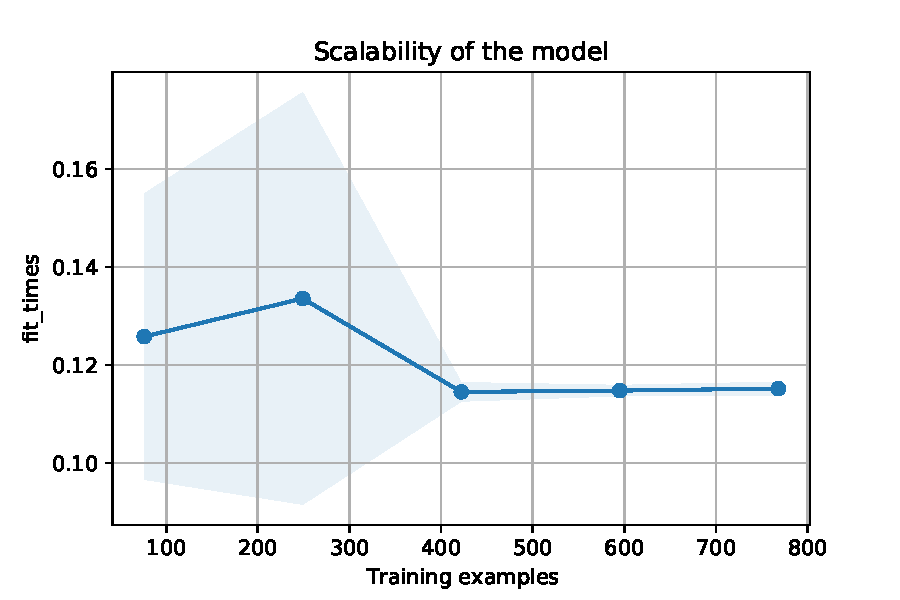
\includegraphics[width=8.5cm]{./code/figures_python/learning_curves/rfc_scalability.pdf}%
\columnbreak
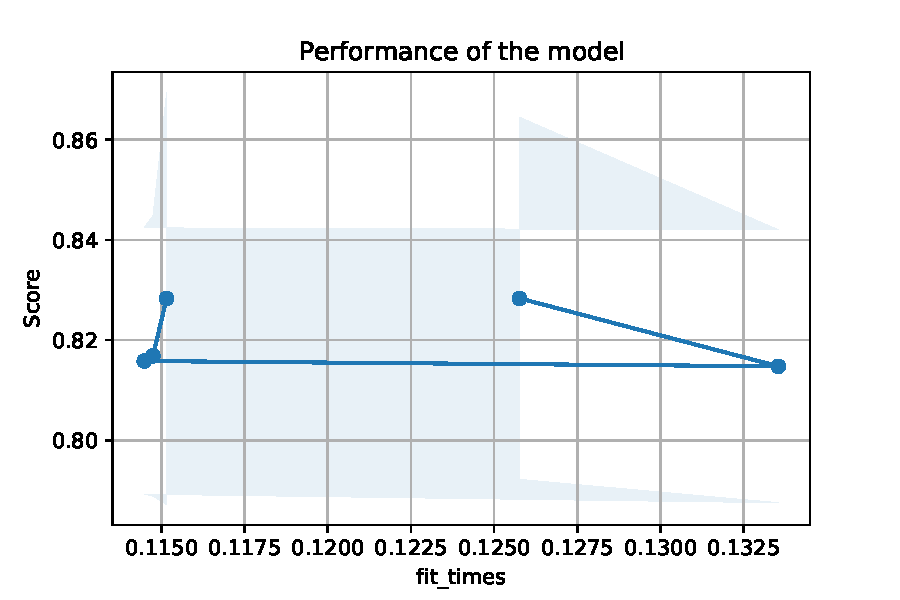
\includegraphics[width=8.5cm]{./code/figures_python/learning_curves/rfc_performance.pdf}%
\end{multicols}
\caption{RFC - Curvas}
\label{rfc:curves}
\end{figure}

%%%%%%%%%%%%%%%
\subsection*{Gradient Boosting}
\addcontentsline{toc}{subsection}{Gradient Boostings}  
\textbf{Boosting} es otra técnica de conjunto para crear una colección de predictores. En esta técnica, los predictores aprenden de manera secuencial y los primeros ajustan modelos simples a los datos y luego analizan los datos para detectar errores. En otras palabras, ajustamos árboles consecutivos (muestra aleatoria) y en cada paso, el objetivo es resolver el error neto del árbol anterior. 

Gradient Boosting es una extensión de Boosting, utiliza un algoritmo de descenso de gradiente que puede optimizar cualquier función de pérdida diferenciable, construye un conjunto de árboles uno por uno y los árboles individuales se suman secuencialmente. El siguiente árbol intenta recuperar la pérdida (diferencia entre los valores reales y previstos).

De igual manera a como hemos hecho con el Random Forest, probamos estos parámetros que nos proporciona la libreria de skelearn \cite{gbc}:

\begin{itemize}
	\item n\_estimators (número de árboles, probaremos  [1,10,50,100,200])
	\item max\_depth (máxima profundidad del árbol, probaremos [1,3,5,8])
\end{itemize}

En la tabla [\ref{gbc:inicial}] mostramos los resultados de nuestra configuración por defecto usando la pipeline y sin preprocesamiento.

\begin{table}[h]
\begin{center}
  \begin{tabular}{|c|c|c|c|}
  \hline
    \multicolumn{4}{|c|}{\textbf{Puntuación configuración por defecto Gradient Boostings}} \\  
    \hline
    \multicolumn{2}{|c|}{\textbf{pipeline}} & \multicolumn{2}{|c|}{\textbf{GradientBoostingClassifier()}}\\    
    \hline
   cross\_val\_score & std & cross\_val\_score & std  \\ 
   \hline
0.819 & 0.03 &0.823 & 0.03  \\ 
\hline
  \end{tabular}
  \end{center}
\caption{GradientBoostingClassifier - Inicial}
\label{gbc:inicial}
\end{table}

En general, hay algunos parámetros con los que puede jugar para reducir el sobreajuste. Lo más fácil de entender conceptualmente es aumentar min\_samples\_split y min\_samples\_leaf. Establecer valores más altos para estos no permitirá que el modelo memorice cómo identificar correctamente una sola pieza de datos o grupos de datos muy pequeños. Para un conjunto de datos grande, colocaría estos valores en alrededor de 50. Se puede hacer una búsqueda en cuadrícula para encontrar valores que funcionen bien para sus datos específicos.

También se puede utilizar submuestra para reducir el sobreajuste y max\_features. Estos parámetros básicamente no permiten que su modelo mire algunos de los datos, lo que le impide memorizarlos.

\begin{table}[ht!]
\begin{center}
\resizebox{\textwidth}{!}{
\begin{tabular}{rrllr}
\toprule
 clf\_\_max\_depth &  clf\_\_n\_estimators & pre\_\_cat\_\_imputer\_cat\_\_strategy & pre\_\_num\_\_imputer\_num\_\_strategy &  Accuracy \\
\midrule
              3 &                  1 &                          median &                          median &  0.835417 \\
              3 &                  1 &                   most\_frequent &                          median &  0.835417 \\
              3 &                  1 &                          median &                            mean &  0.833333 \\
              3 &                  1 &                   most\_frequent &                            mean &  0.833333 \\
              1 &                 50 &                   most\_frequent &                          median &  0.833333 \\
              1 &                 50 &                          median &                          median &  0.833333 \\
              1 &                200 &                          median &                          median &  0.831250 \\
              1 &                200 &                   most\_frequent &                          median &  0.831250 \\
              1 &                 50 &                   most\_frequent &                            mean &  0.827083 \\
              1 &                 50 &                          median &                            mean &  0.827083 \\
              1 &                100 &                   most\_frequent &                          median &  0.825000 \\
              1 &                100 &                          median &                          median &  0.825000 \\
              1 &                  1 &                   most\_frequent &                          median &  0.822917 \\
              1 &                200 &                          median &                            mean &  0.822917 \\
              1 &                200 &                   most\_frequent &                            mean &  0.822917 \\
              1 &                  1 &                   most\_frequent &                            mean &  0.822917 \\
              1 &                 10 &                          median &                          median &  0.822917 \\
              1 &                 10 &                          median &                            mean &  0.822917 \\
\bottomrule
\end{tabular}
}
\end{center}
\caption{GBC - Accuracy}
\label{gbc:table}
\end{table}

\begin{figure}[ht!]
\begin{multicols}{2}
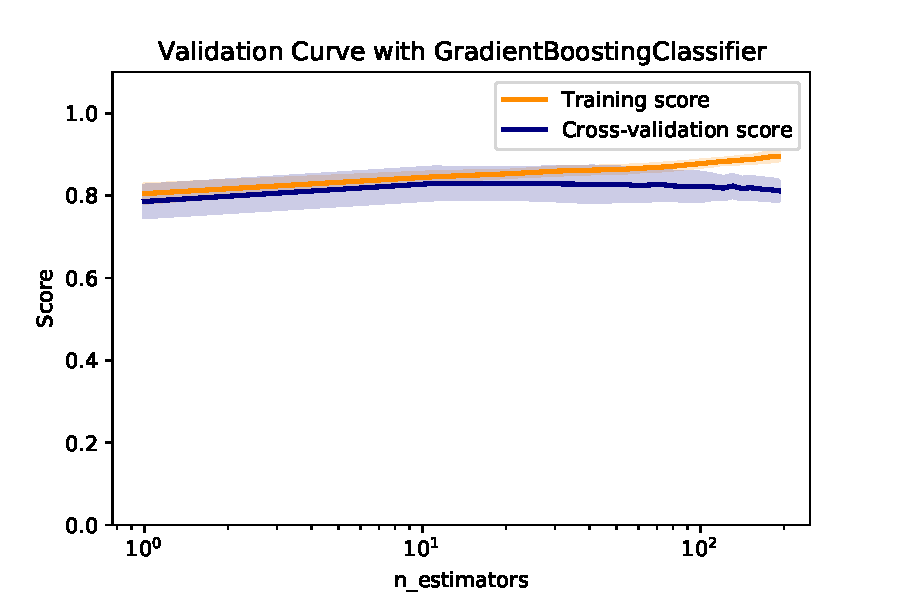
\includegraphics[width=8.5cm]{./code/figures_python/validation_curves/gbc.pdf}%
\columnbreak
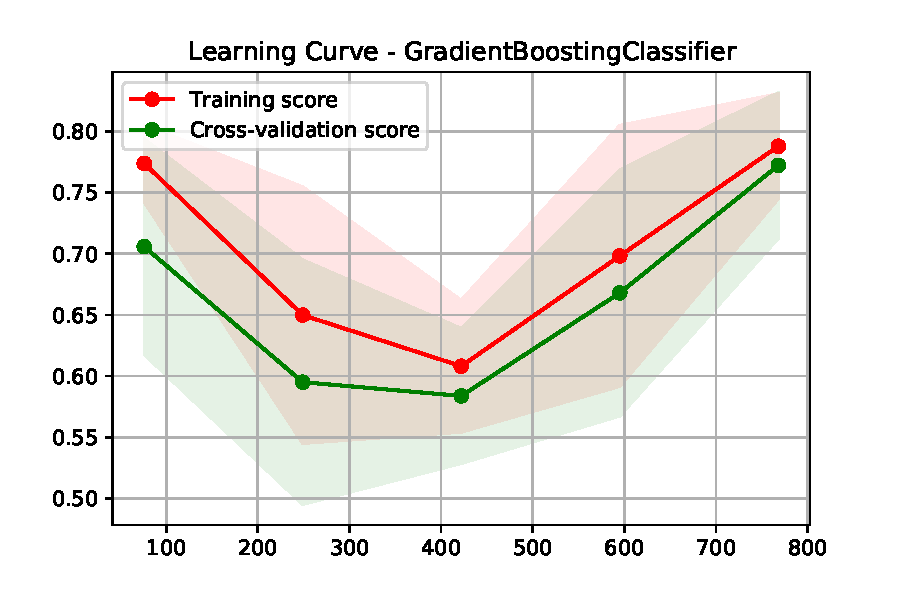
\includegraphics[width=8.5cm]{./code/figures_python/learning_curves/gbc.pdf}%
\end{multicols}

\begin{multicols}{2}
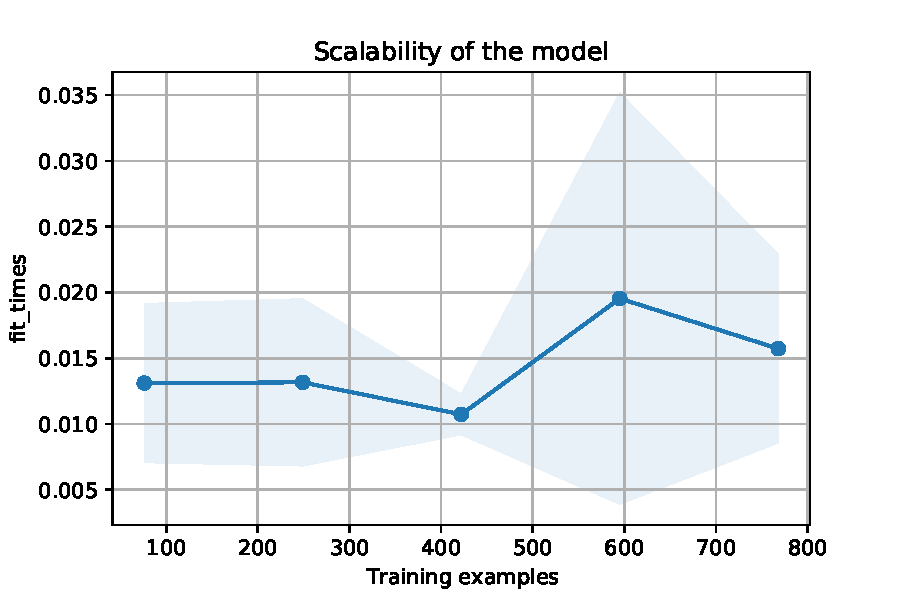
\includegraphics[width=8.5cm]{./code/figures_python/learning_curves/gbc_scalability.pdf}%
\columnbreak
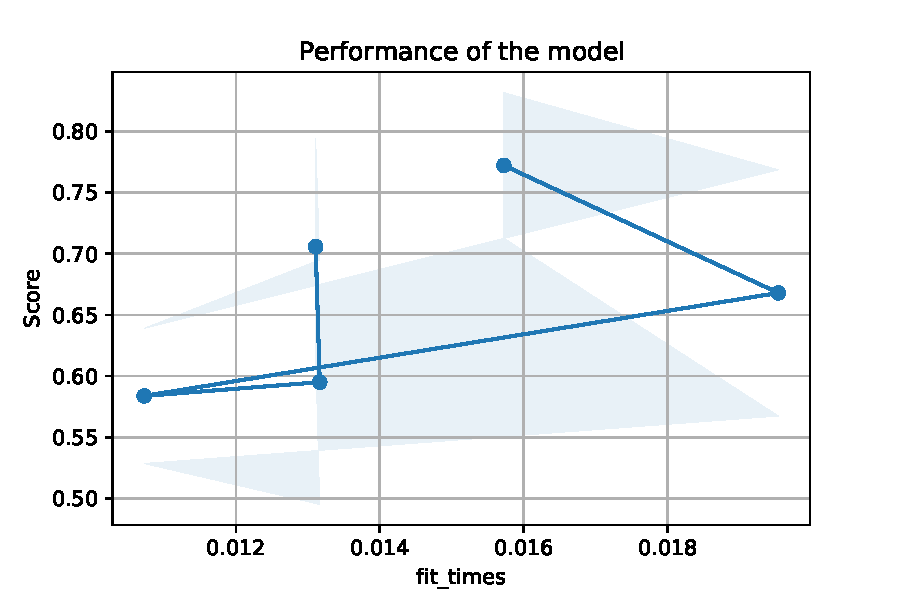
\includegraphics[width=8.5cm]{./code/figures_python/learning_curves/gbc_performance.pdf}%
\end{multicols}
\caption{GBC - Curvas}
\label{gbc:curves}
\end{figure}
%%%%%%%%%%%%%%%%%%%%%%%%%%%%%%%%%%%%
\chapter*{Resultados obtenidos}
\addcontentsline{toc}{chapter}{Resultados obtenidos}  

En esta sección mostramos el código de la creación del modelo, nos quedamos con la mejor configuración de las mostradas anteriormente junto a la pipeline explicada para el preprocesamiento, vemos una tabla con los resultados obtenidos por el algoritmo, tablas de errores (precisión), matrices de confusión, y hacemos plot del ROC. 

%%%%%%%%%%%%%%%
\section*{Logistic Regression}
\addcontentsline{toc}{section}{Logistic Regression}  

Vemos el código de creación del modelo con nuestra mejor combinación de parámetros en la Figura [\ref{lr:code}], en la tabla [\ref{lr:precision}] las principales métricas de clasificación. En la figura [\ref{lr:roc}] mostramos el Receiver Operating Characteristic (ROC) para evaluar la calidad de salida del clasificador y finalmente la matriz de confusión en la figura [\ref{lr:matrix}]

\begin{figure}[ht]
 \begin{lstlisting}
Best estimator: Pipeline(steps=[('pre',
	ColumnTransformer(transformers=[('cat',Pipeline(steps=[
		('imputer_cat',SimpleImputer(strategy='most_frequent')),
		('onehot', OneHotEncoder(handle_unknown='ignore'))]), ['Shape']),
														('num', Pipeline(steps=[
		('imputer_num',SimpleImputer()),
		('scaler',StandardScaler())]),['BI-RADS', 'Age', 'Margin', 'Density'])])),
                ('clf', LogisticRegression(C=0.01, random_state=10,solver='newton-cg'))])
                
cross_val score y std: (0.8335276338514681, 0.032319847105984616)
 \end{lstlisting}
 \caption{LogisticRegression - Code}
 \label{lr:code}
 \end{figure}

\begin{table}[htp]
\begin{center}
\begin{tabular}{lrrrr}
\toprule
{} &  precision &    recall &  f1-score &     support \\
\midrule
0 (benigno) &   0.833333 &  0.855513 &  0.844278 &  263.000000 \\
1 (maligno) &   0.819905 &  0.793578 &  0.806527 &  218.000000 \\
accuracy     &   0.827443 &  0.827443 &  0.827443 &    0.827443 \\
macro avg    &   0.826619 &  0.824546 &  0.825402 &  481.000000 \\
weighted avg &   0.827247 &  0.827443 &  0.827168 &  481.000000 \\
\bottomrule
\end{tabular}
\end{center}
\caption{LogisticRegression - Tabla de errores}
\label{lr:precision}
\end{table}

\begin{figure}[htp]
\begin{center}
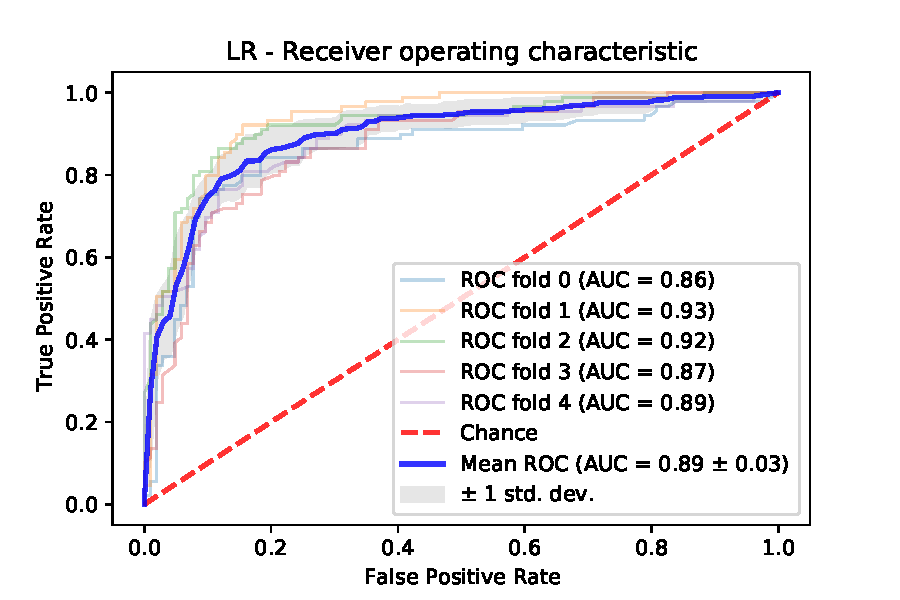
\includegraphics[width=8.5cm]{./code/figures_python/roc/lr.pdf}%
\end{center}
 \caption{LogisticRegression - ROC}
 \label{lr:roc}
 \end{figure}
 
\begin{figure}[htp]
\begin{multicols}{2}
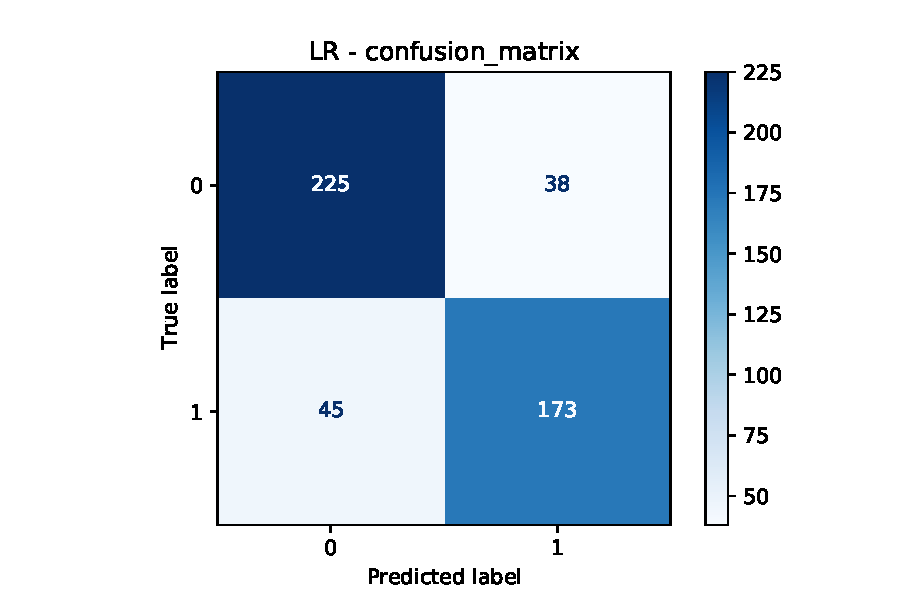
\includegraphics[width=8.5cm]{./code/figures_python/confusion_matrix/lr.pdf}%
\columnbreak
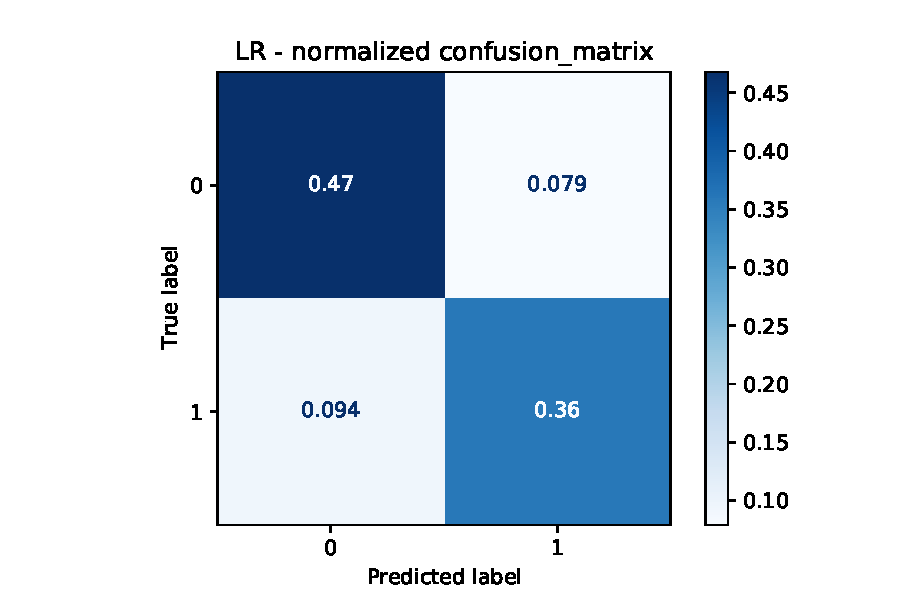
\includegraphics[width=8.5cm]{./code/figures_python/confusion_matrix/lr_normalized.pdf}%
\end{multicols}
 \caption{LogisticRegression - Confusion Matrix}
 \label{lr:matrix}
 \end{figure}
 
%%%%%%%%%%%%%%%
\section*{KNeighborsClassifier}
\addcontentsline{toc}{section}{KNeighborsClassifier}  

Vemos el código de creación del modelo con nuestra mejor combinación de parámetros en la Figura [\ref{knn:code}], en la tabla [\ref{knn:precision}] las principales métricas de clasificación. En la figura [\ref{knn:roc}] mostramos el Receiver Operating Characteristic (ROC) para evaluar la calidad de salida del clasificador y finalmente la matriz de confusión en la figura [\ref{knn:matrix}].

\begin{figure}[ht]
 \begin{lstlisting}
Best estimator: Pipeline(steps=[('pre',
	ColumnTransformer(transformers=[('cat',Pipeline(steps=[
		('imputer_cat',SimpleImputer(strategy='most_frequent')),
		('onehot', OneHotEncoder(handle_unknown='ignore'))]), ['Shape']),
														('num', Pipeline(steps=[
		('imputer_num',SimpleImputer()),
		('scaler',StandardScaler())]),['BI-RADS', 'Age', 'Margin', 'Density'])])),
                ('clf', KNeighborsClassifier(metric='manhattan', n_neighbors=6))])
                
cross_val score y std: (0.8179134283246977, 0.026233632645637096)
 \end{lstlisting}
 \caption{KNeighborsClassifier - Code}
 \label{knn:code}
 \end{figure}

\begin{table}[htp]
\begin{center}
\begin{tabular}{lrrrr}
\toprule
{} &  precision &    recall &  f1-score &     support \\
\midrule
0            &   0.815603 &  0.874525 &  0.844037 &  263.000000 \\
1            &   0.834171 &  0.761468 &  0.796163 &  218.000000 \\
accuracy     &   0.823285 &  0.823285 &  0.823285 &    0.823285 \\
macro avg    &   0.824887 &  0.817996 &  0.820100 &  481.000000 \\
weighted avg &   0.824018 &  0.823285 &  0.822339 &  481.000000 \\
\bottomrule
\end{tabular}
\end{center}
\caption{KNeighborsClassifier - Tabla de errores}
\label{knn:precision}
\end{table}


\begin{figure}[htp]
\begin{center}
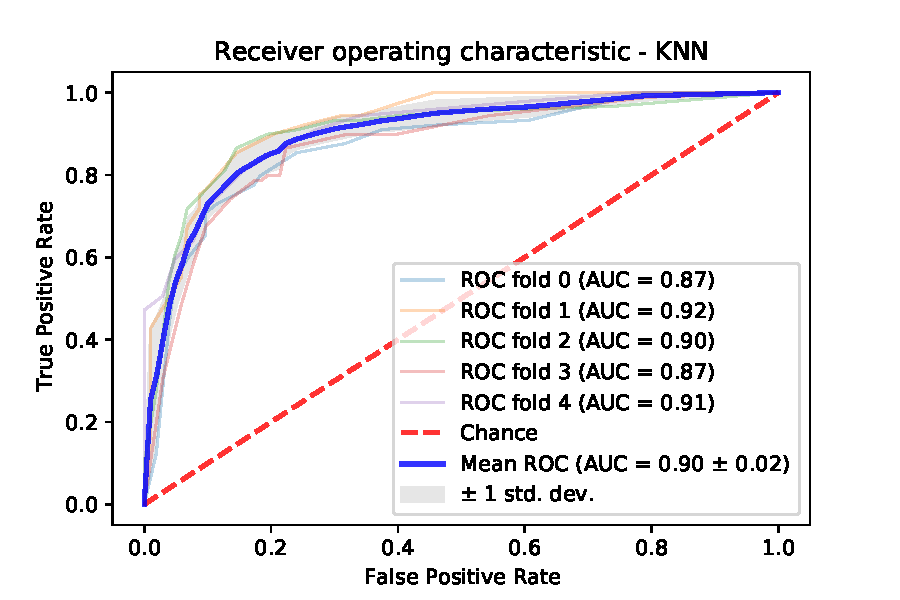
\includegraphics[width=8.5cm]{./code/figures_python/roc/knn.pdf}%
\end{center}
 \caption{KNeighborsClassifier - ROC}
 \label{knn:roc}
 \end{figure}
 
\begin{figure}[htp]
\begin{multicols}{2}
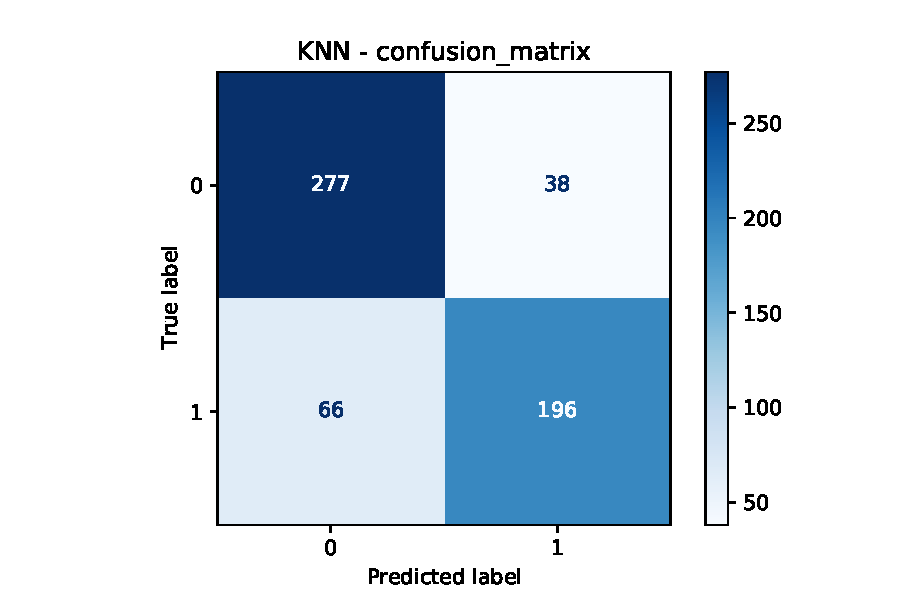
\includegraphics[width=8.5cm]{./code/figures_python/confusion_matrix/knn.pdf}%
\columnbreak
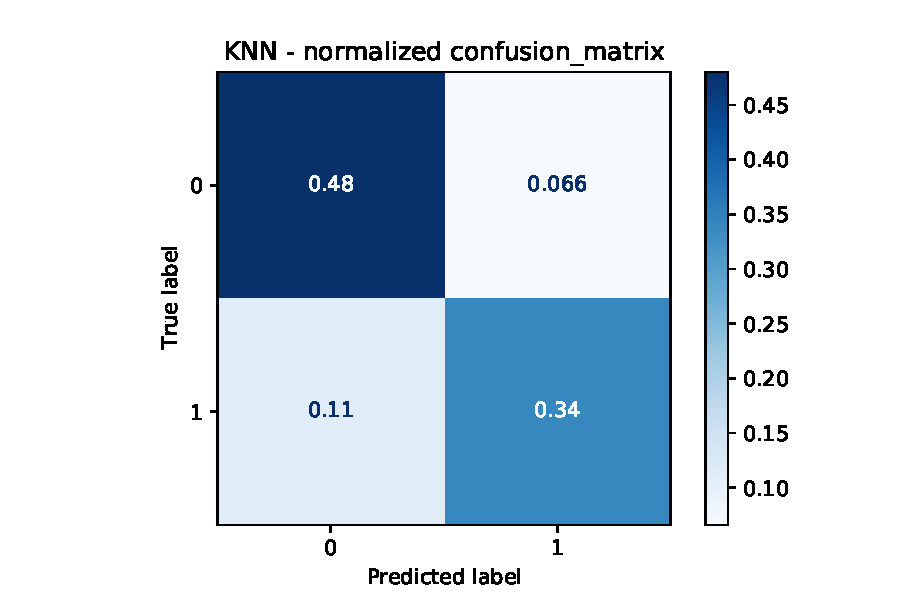
\includegraphics[width=8.5cm]{./code/figures_python/confusion_matrix/knn_normalized.pdf}%
\end{multicols}
 \caption{KNeighborsClassifier - Confusion Matrix}
  \label{knn:matrix}
 \end{figure}



%%%%%%%%%%%%%%%
\section*{Support Vector Machines}
\addcontentsline{toc}{section}{Support Vector Machines}  


Vemos el código de creación del modelo con nuestra mejor combinación de parámetros en la Figura [\ref{svc:code}], en la tabla [\ref{svc:precision}] las principales métricas de clasificación. En la figura [\ref{svc:roc}] mostramos el Receiver Operating Characteristic (ROC) para evaluar la calidad de salida del clasificador y finalmente la matriz de confusión en la figura [\ref{svc:matrix}].

\begin{figure}[ht]
 \begin{lstlisting}
Best estimator: Pipeline(steps=[('pre',
	ColumnTransformer(transformers=[('cat',Pipeline(steps=[
		('imputer_cat',SimpleImputer(strategy='most_frequent')),
		('onehot', OneHotEncoder(handle_unknown='ignore'))]), ['Shape']),
														('num', Pipeline(steps=[
		('imputer_num',SimpleImputer()),
		('scaler',StandardScaler())]),['BI-RADS', 'Age', 'Margin', 'Density'])])),
 ('clf', SVC(C=1, gamma='auto', random_state=10))])
                
cross_val score y std: (0.8283246977547496, 0.03887076020885105)
 \end{lstlisting}
 \caption{SVC - Code}
 \label{svc:code}
 \end{figure}

\begin{table}[htp]
\begin{center}
\begin{tabular}{lrrrr}
\toprule
{} &  precision &    recall &  f1-score &     support \\
\midrule
0            &   0.834559 &  0.863118 &  0.848598 &  263.000000 \\
1            &   0.827751 &  0.793578 &  0.810304 &  218.000000 \\
accuracy     &   0.831601 &  0.831601 &  0.831601 &    0.831601 \\
macro avg    &   0.831155 &  0.828348 &  0.829451 &  481.000000 \\
weighted avg &   0.831473 &  0.831601 &  0.831243 &  481.000000 \\
\bottomrule
\end{tabular}
\end{center}
\caption{SVC - Tabla de errores}
\label{svc:precision}
\end{table}

\begin{figure}[htp]
\begin{center}
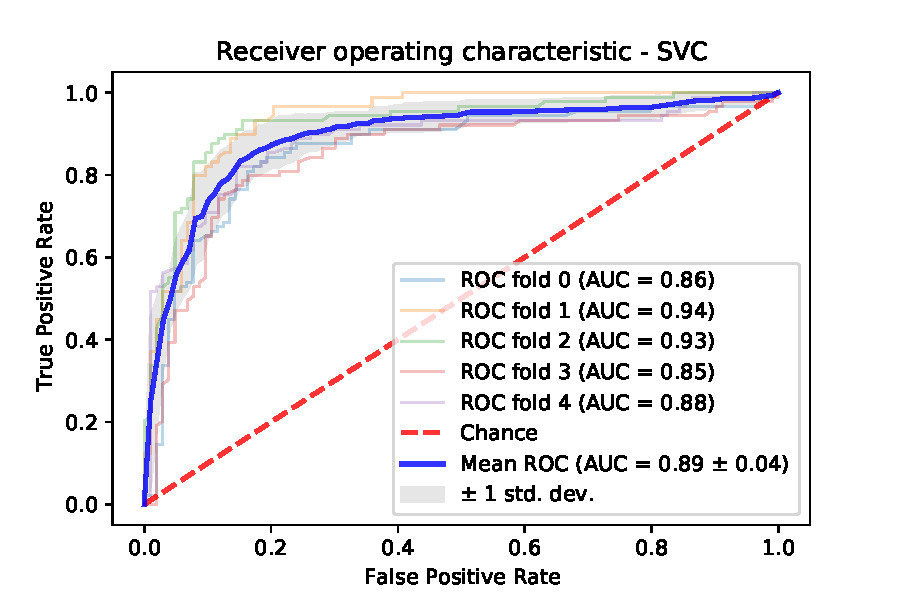
\includegraphics[width=8.5cm]{./code/figures_python/roc/svc.pdf}%
\end{center}
 \caption{SVC - ROC}
 \label{svc:roc}
 \end{figure}
 
\begin{figure}[htp]
\begin{multicols}{2}
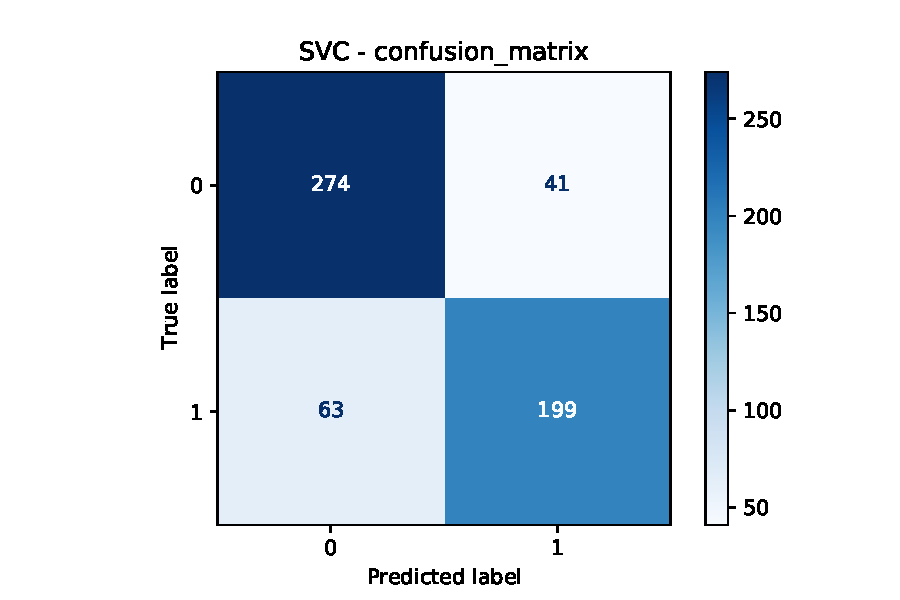
\includegraphics[width=8.5cm]{./code/figures_python/confusion_matrix/svc.pdf}%
\columnbreak
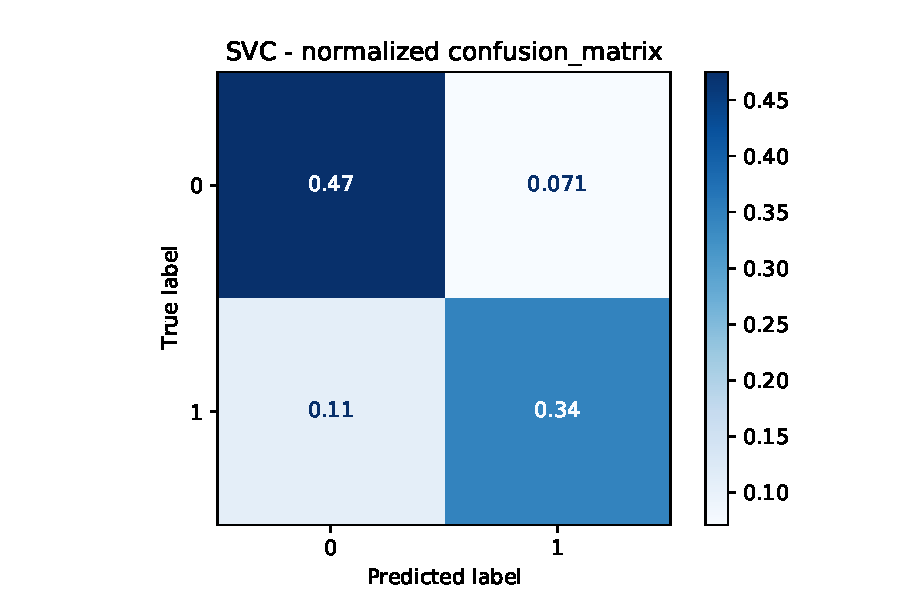
\includegraphics[width=8.5cm]{./code/figures_python/confusion_matrix/svc_normalized.pdf}%
\end{multicols}
 \caption{SVC - Confusion Matrix}
  \label{svc:matrix}
 \end{figure}
 
 %%%%%%%%%%%%%%%
\section*{Gradient Boosting}
\addcontentsline{toc}{section}{Gradient Boostings}  

Vemos el código de creación del modelo con nuestra mejor combinación de parámetros en la Figura [\ref{gbc:code}], en la tabla [\ref{gbc:precision}] las principales métricas de clasificación. En la figura [\ref{gbc:roc}] mostramos el Receiver Operating Characteristic (ROC) para evaluar la calidad de salida del clasificador y finalmente la matriz de confusión en la figura [\ref{gbc:matrix}].

\begin{figure}[ht]
 \begin{lstlisting}
Best estimator: Pipeline(steps=[('pre',
	ColumnTransformer(transformers=[('cat',Pipeline(steps=[
		('imputer_cat',SimpleImputer(strategy='most_frequent')),
		('onehot', OneHotEncoder(handle_unknown='ignore'))]), ['Shape']),
														('num', Pipeline(steps=[
		('imputer_num',SimpleImputer(strategy='median')),
		('scaler',StandardScaler())]),['BI-RADS', 'Age', 'Margin', 'Density'])])),
		('clf',GradientBoostingClassifier(n_estimators=1, random_state=10))])
                
cross_val score y std: (0.785627158894646, 0.03710160085379686)
 \end{lstlisting}
 \caption{GBC - Code}
 \label{gbc:code}
 \end{figure}

\begin{table}[htp]
\begin{center}
\begin{tabular}{lrrrr}
\toprule
{} &  precision &    recall &  f1-score &     support \\
\midrule
0 (benigno) &   0.725948 &  0.946768 &  0.821782 &  263.000000 \\
1 (maligno) &   0.898551 &  0.568807 &  0.696629 &  218.000000 \\
accuracy     &   0.775468 &  0.775468 &  0.775468 &    0.775468 \\
macro avg    &   0.812249 &  0.757788 &  0.759206 &  481.000000 \\
weighted avg &   0.804175 &  0.775468 &  0.765060 &  481.000000 \\
\bottomrule
\end{tabular}
\end{center}
\caption{GBC - Tabla de errores}
\label{gbc:precision}
\end{table}

\begin{figure}[htp]
\begin{center}
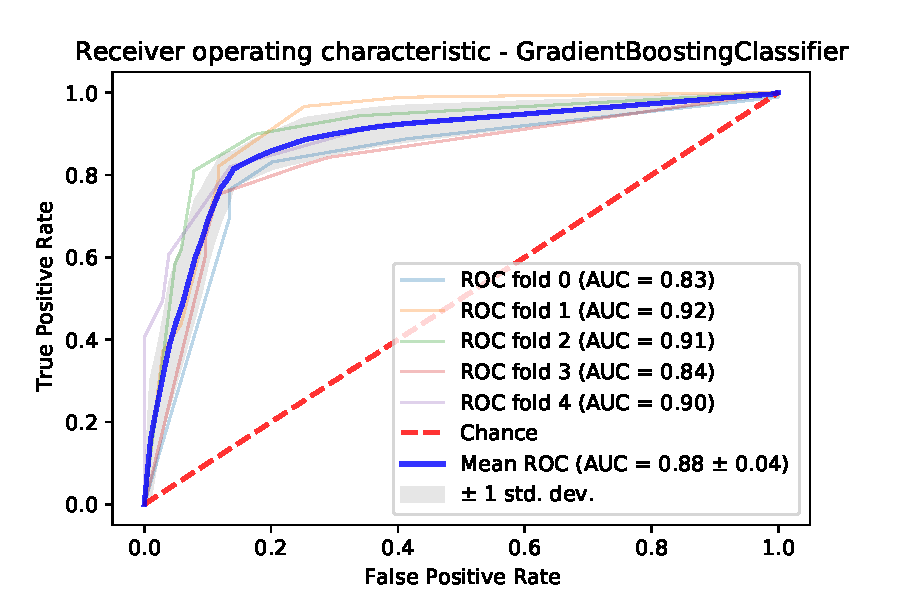
\includegraphics[width=8.5cm]{./code/figures_python/roc/gbc.pdf}%
\end{center}
 \caption{GBC - ROC}
 \label{gbc:roc}
 \end{figure}
 
\begin{figure}[htp]
\begin{multicols}{2}
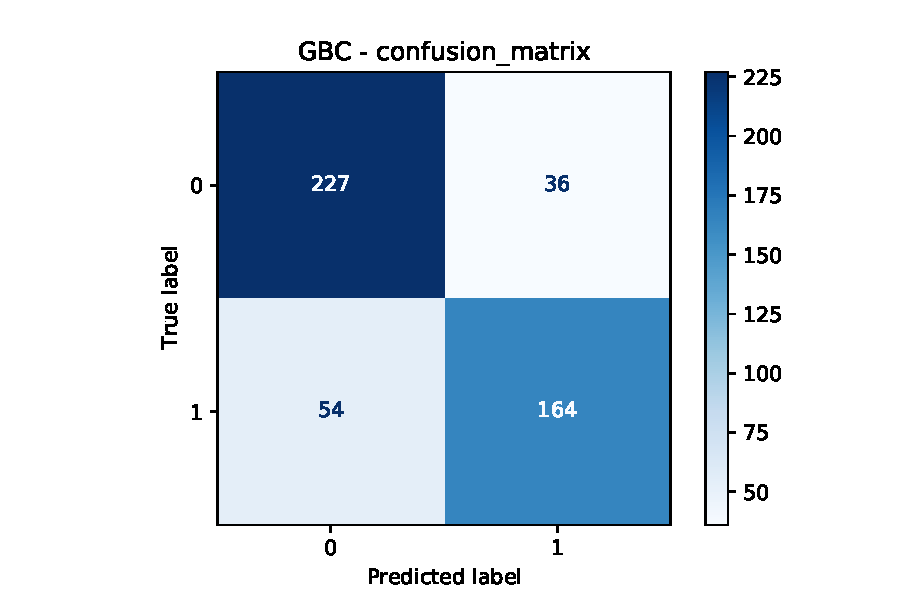
\includegraphics[width=8.5cm]{./code/figures_python/confusion_matrix/gbc.pdf}%
\columnbreak
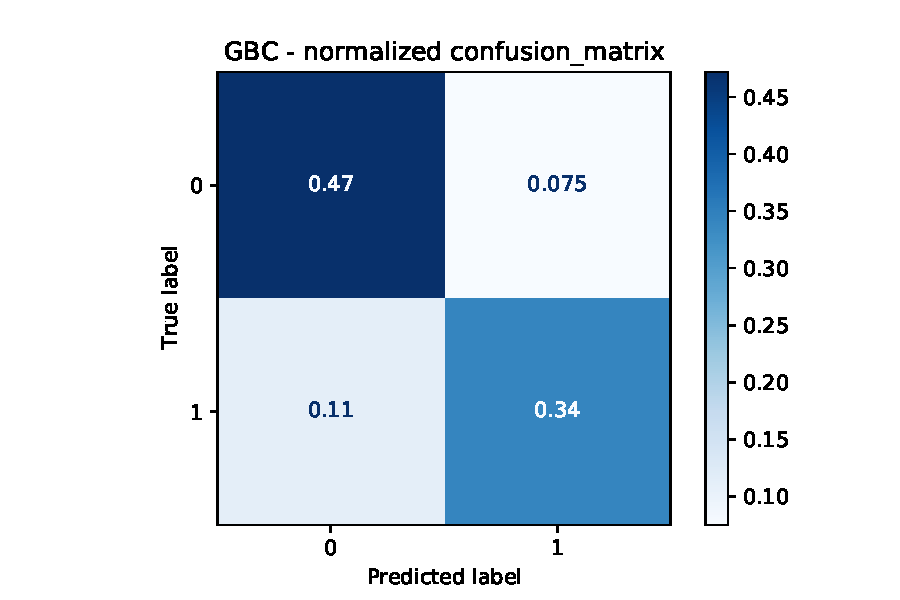
\includegraphics[width=8.5cm]{./code/figures_python/confusion_matrix/gbc_normalized.pdf}%
\end{multicols}
 \caption{GBC - Confusion Matrix}
  \label{gbc:matrix}
 \end{figure}

%%%%%%%%%%%%%%%
\section*{RandomForestClassifier}
\addcontentsline{toc}{section}{RandomForestClassifier}  

Vemos el código de creación del modelo con nuestra mejor combinación de parámetros en la Figura [\ref{rfc:code}], en la tabla [\ref{rfc:precision}] las principales métricas de clasificación. En la figura [\ref{rfc:roc}] mostramos el Receiver Operating Characteristic (ROC) para evaluar la calidad de salida del clasificador y finalmente la matriz de confusión en la figura [\ref{rfc:matrix}].

\begin{figure}[ht]
 \begin{lstlisting}
Best estimator: Pipeline(steps=[('pre',
	ColumnTransformer(transformers=[('cat',Pipeline(steps=[
		('imputer_cat',SimpleImputer(strategy='most_frequent')),
		('onehot', OneHotEncoder(handle_unknown='ignore'))]), ['Shape']),
														('num', Pipeline(steps=[
		('imputer_num',SimpleImputer(strategy='median')),
		('scaler',StandardScaler())]),['BI-RADS', 'Age', 'Margin', 'Density'])])),
		('clf', RandomForestClassifier(max_depth=1, random_state=10))])
                
cross_val score y std: (0.8314389032815198, 0.041161211805022364)
 \end{lstlisting}
 \caption{RFC - Code}
 \label{rfc:code}
 \end{figure}

\begin{table}[htp]
\begin{center}
\begin{tabular}{lrrrr}
\toprule
{} &  precision &    recall &  f1-score &     support \\
\midrule
0(benigno)&   0.786667 &  0.897338 &  0.838366 &  263.000000 \\
1(maligno)&   0.850829 &  0.706422 &  0.771930 &  218.000000 \\
accuracy     &   0.810811 &  0.810811 &  0.810811 &    0.810811 \\
macro avg    &   0.818748 &  0.801880 &  0.805148 &  481.000000 \\
weighted avg &   0.815746 &  0.810811 &  0.808256 &  481.000000 \\
\bottomrule
\end{tabular}
\end{center}
\caption{RFC - Tabla de errores}
\label{rfc:precision}
\end{table}

\begin{figure}[htp]
\begin{center}
\includegraphics[width=8.5cm]{./code/figures_python/roc/rfc.pdf}%
\end{center}
 \caption{RFC - ROC}
 \label{rfc:roc}
 \end{figure}
 
\begin{figure}[htp]
\begin{multicols}{2}
\includegraphics[width=8.5cm]{./code/figures_python/confusion_matrix/rfc.pdf}%
\columnbreak
\includegraphics[width=8.5cm]{./code/figures_python/confusion_matrix/rfc_normalized.pdf}%
\end{multicols}
 \caption{RFC - Confusion Matrix}
  \label{rfc:matrix}
 \end{figure}


%%%%%%%%%%%%%%%%%%%%%%%%%%%%%%%%%%%%
\chapter*{Análisis de resultados}
\addcontentsline{toc}{chapter}{Análisis de resultados}  

Comparamos los resultados globales de cada mejor estimador de cada tipo comentado hasta ahora se puede ver una comparación con distintas medidas en la tabla [\ref{comp:general}], donde los resultados son la media haciendo validación cruzada con 5 particiones y distintos tipos de scores, también mostramos un boxplot en la figura [\ref{comp:alghoritms}]

Nuestros modelos tienen una varianza muy baja, lo que en realidad es muy bueno, ya que eso significa que la predicción que obtuvimos en un conjunto de prueba no es casualidad.

Las curvas ROC suelen presentar una tasa de verdaderos positivos en el eje Y y una tasa de falsos positivos en el eje X. Esto significa que la esquina superior izquierda de la gráfica es el punto "ideal": una tasa de falsos positivos de cero y una tasa de verdaderos positivos de uno. Esto no es muy realista, pero significa que un área más grande bajo la curva (AUC) suele ser mejor.

La "inclinación" de las curvas ROC también es importante, ya que es ideal para maximizar la tasa de verdaderos positivos y minimizar la tasa de falsos positivos.

\begin{table}[ht]
\begin{center}
\begin{tabular}{lrrrr}
\toprule
{} &  accuracy &precision &    recall &  f1-score \\
\midrule
LR &  0.833528 (0.03) &  0.819461 (0.04) &  0.824719 (0.08) &  0.819254 (0.03) \\
KNN &   0.817913 (0.03) &  0.792745 (0.04)&  0.764045 (0.09) &  0.835127 (0.05) \\
SVC     &   0.828325 (0.04) &  0.807295 (0.05) &  0.791011 (0.096) &   0.833651 (0.042) \\
GBC    &   0.785627 (0.04) & 0.723419 (0.08) &  0.631461 (0.13) &  0.884859 (0.07) \\
RFC    &   0.831439 (0.04) &   0.799719 (0.07) &  0.755056 (0.126) &  0.873664 (0.06)\\
\bottomrule
\end{tabular}
\end{center}
\caption{Comparación de resultados}
\label{comp:general}
\end{table}


LR(LogisticRegression) , KNN (KneighborsClassifier), SVC, GBC (GradientBoostingClassifier) y RFC (RandomForestClassifier)
\begin{figure}[ht]
\begin{multicols}{2}
\includegraphics[width=8.5cm]{./code/figures_python/comparison/accuracy.pdf}%
\columnbreak
\includegraphics[width=8.5cm]{./code/figures_python/comparison/precision.pdf}%
\end{multicols}
\begin{multicols}{2}
\includegraphics[width=8.5cm]{./code/figures_python/comparison/f1.pdf}%
\columnbreak
\includegraphics[width=8.5cm]{./code/figures_python/comparison/recall.pdf}%
\end{multicols}
 \caption{Boxplot de los distintos algoritmos con distintos tipos de puntuación.}
  \label{comp:alghoritms}
 \end{figure}
 
 \begin{figure}[ht]
\includegraphics[width=\textwidth]{./code/figures_python/comparison/roc.pdf}%
 \caption{ROC de todos los algoritmos}
  \label{comp:roc}
 \end{figure}
 
%%%%%%%%%%%%%%%%%%%%%%%%%%%%%%%%%%%%
\chapter*{Interpretación de resultados}
\addcontentsline{toc}{chapter}{Interpretación de resultados}  

Considerando nuestro problema de clasificar tumores como maligno o benigno, querremos que el modelo minimice el número de falsos negativo. En este caso, es posible que esté bien con un modelo que tenga una alta recall, pero poca precision. Luego la regresión logística funciona muy bien para nuestro caso, además es un modelo simple, en general es mejor coger modelos simples faciles de explicar si obtienen buenos resultados que coger los complejos. El porque de unos algoritmos funciona mejor que otros puede ser por que lo que más influye son las hipótesis que asumen los algoritmos, algunos asumen hipótesis de normalidad mientras otros asumen otras distribuciones, cuando las hipótesis no las cumplen los datos de partida el resultado empeora. Si utilizamos árboles debemos de tener cuidado con las decisiones que se toman en los nodos, los árboles pueden no llevarse bien con los datos continuos, en este caso nuestra clase Age puede afectar negativamente a estos modelos.

RandomForest y GradientBoosting funcionan bien con variables categóricas u ordinales, los otros están basados en distancias que funcionan muy bien para clasificación binaria. Regresión logística también funciona muy bien para clasificación binaria, aparte de que puede usar distintas normas (Lasso o Ridge) para evitar el overfitting.

%% bibliography
\medskip

\printbibliography[
heading=bibintoc,
title={Referencias}
]


\end{document}
